\documentclass[]{article}
\usepackage{lmodern}
\usepackage{amssymb,amsmath}
\usepackage{ifxetex,ifluatex}
\usepackage{fixltx2e} % provides \textsubscript
\ifnum 0\ifxetex 1\fi\ifluatex 1\fi=0 % if pdftex
  \usepackage[T1]{fontenc}
  \usepackage[utf8]{inputenc}
\else % if luatex or xelatex
  \ifxetex
    \usepackage{mathspec}
  \else
    \usepackage{fontspec}
  \fi
  \defaultfontfeatures{Ligatures=TeX,Scale=MatchLowercase}
\fi
% use upquote if available, for straight quotes in verbatim environments
\IfFileExists{upquote.sty}{\usepackage{upquote}}{}
% use microtype if available
\IfFileExists{microtype.sty}{%
\usepackage{microtype}
\UseMicrotypeSet[protrusion]{basicmath} % disable protrusion for tt fonts
}{}
\usepackage[margin=1in]{geometry}
\usepackage{hyperref}
\hypersetup{unicode=true,
            pdfborder={0 0 0},
            breaklinks=true}
\urlstyle{same}  % don't use monospace font for urls
\usepackage{graphicx,grffile}
\makeatletter
\def\maxwidth{\ifdim\Gin@nat@width>\linewidth\linewidth\else\Gin@nat@width\fi}
\def\maxheight{\ifdim\Gin@nat@height>\textheight\textheight\else\Gin@nat@height\fi}
\makeatother
% Scale images if necessary, so that they will not overflow the page
% margins by default, and it is still possible to overwrite the defaults
% using explicit options in \includegraphics[width, height, ...]{}
\setkeys{Gin}{width=\maxwidth,height=\maxheight,keepaspectratio}
\IfFileExists{parskip.sty}{%
\usepackage{parskip}
}{% else
\setlength{\parindent}{0pt}
\setlength{\parskip}{6pt plus 2pt minus 1pt}
}
\setlength{\emergencystretch}{3em}  % prevent overfull lines
\providecommand{\tightlist}{%
  \setlength{\itemsep}{0pt}\setlength{\parskip}{0pt}}
\setcounter{secnumdepth}{0}
% Redefines (sub)paragraphs to behave more like sections
\ifx\paragraph\undefined\else
\let\oldparagraph\paragraph
\renewcommand{\paragraph}[1]{\oldparagraph{#1}\mbox{}}
\fi
\ifx\subparagraph\undefined\else
\let\oldsubparagraph\subparagraph
\renewcommand{\subparagraph}[1]{\oldsubparagraph{#1}\mbox{}}
\fi

%%% Use protect on footnotes to avoid problems with footnotes in titles
\let\rmarkdownfootnote\footnote%
\def\footnote{\protect\rmarkdownfootnote}

%%% Change title format to be more compact
\usepackage{titling}

% Create subtitle command for use in maketitle
\providecommand{\subtitle}[1]{
  \posttitle{
    \begin{center}\large#1\end{center}
    }
}

\setlength{\droptitle}{-2em}

  \title{}
    \pretitle{\vspace{\droptitle}}
  \posttitle{}
    \author{}
    \preauthor{}\postauthor{}
    \date{}
    \predate{}\postdate{}
  
\usepackage{booktabs}
\usepackage{longtable}
\usepackage{array}
\usepackage{multirow}
\usepackage{wrapfig}
\usepackage{float}
\usepackage{colortbl}
\usepackage{pdflscape}
\usepackage{tabu}
\usepackage{threeparttable}
\usepackage{threeparttablex}
\usepackage[normalem]{ulem}
\usepackage{makecell}
\usepackage{xcolor}

\begin{document}

\hypertarget{velocity}{%
\section{\texorpdfstring{Velocity (\emph{v}): using rate-of-change of
system trajectory to identify abrupt
changes}{Velocity (v): using rate-of-change of system trajectory to identify abrupt changes}}\label{velocity}}

\hypertarget{introduction}{%
\subsection{Introduction}\label{introduction}}

When, how and why ecological systems exhibit abrupt changes is a
hallmark of modern ecological research, and changes which are unexpected
and undesirable can have undesirable downstream consequences on, e.g.,
ecosytem services, biodiversity, and human well-being. Quantitatively
detecting and forecasting these changes, however, has yet to be
accomplished for most ecological systems {[}Chapter
\textbackslash{}@ref(rdmReview); @ratajczak2018abrupt{]}. Moving from
abrupt change methods requiring highly descriptive models and \emph{a
priori} assumptions of the state variable responses to drivers to
methods requiring few, if any, \emph{a priori} assumptions or knowledge
is increasingly necessary for forecasting and managing complex
ecosystems under an era of intensifying anthropogenic pressures.

A few broad classes of quantitative approaches exist for quantitatively
identifying abrupt changes in complex ecosystems. First, one can use
simple mathematical models to describe the system and statistically test
for discontinuities in the observed variables {[}e.g., in coral reefs,
@mumby2013evidence{]}. Although mathematical representations are ideal,
very rarely are ecological systems easily and well-described by them and
often fail to meet the assumptions of the model. Second, we can track
changes in the mean or variance of state variables to identify
departures from the norm {[}e.g., early-warning indicators such as
variance and variance index, @brock\_variance\_2006{]}. Much like the
mathematical modelling approach, these early-warning indicators have
shown to be useful in some simple driver-response systems {[}e.g., lake
eutrophication @carpenter\_leading\_2008{]}, but are unreliable in other
empirical systems {[}e.g.,
@perretti2012regime;@dutta2018robustness;@dakos2012robustness{]}. The
last type of approach is the model-free approach
{[}@dakos\_methods\_2012; Ch. @ref(rdmReview){]}. This group of abrupt
change indicators can incorporate multiple state variables, and ideally
requires no \emph{a priori} assumptions about the expected
driver-response relationships, or even about the drivers at all. It is
this class of abrupt change indicators to which this chapter
contributes.

\hypertarget{tracking-ecosystem-trajectory-through-time-to-explore-system-dynamics}{%
\subsubsection{Tracking ecosystem trajectory through time to explore
system
dynamics}\label{tracking-ecosystem-trajectory-through-time-to-explore-system-dynamics}}

\begin{figure}

{\centering 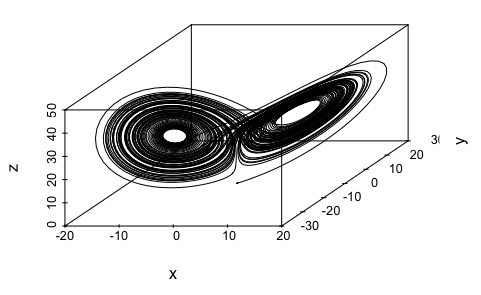
\includegraphics[width=0.55\linewidth]{E:/GitHub/myDissertation/chapterFiles/velocity/figsCalledInDiss/lorenz3D} 

}

\caption{An example solution of the Lorenz ('butterfly') represented in 3-dimensional phase-space. Phase plots are typically used to visualize stable areas within a system's trajectory but reconstruction requires the difference models to be known and parameterized.}\label{fig:lorenz3D}
\end{figure}
\begin{figure}

{\centering 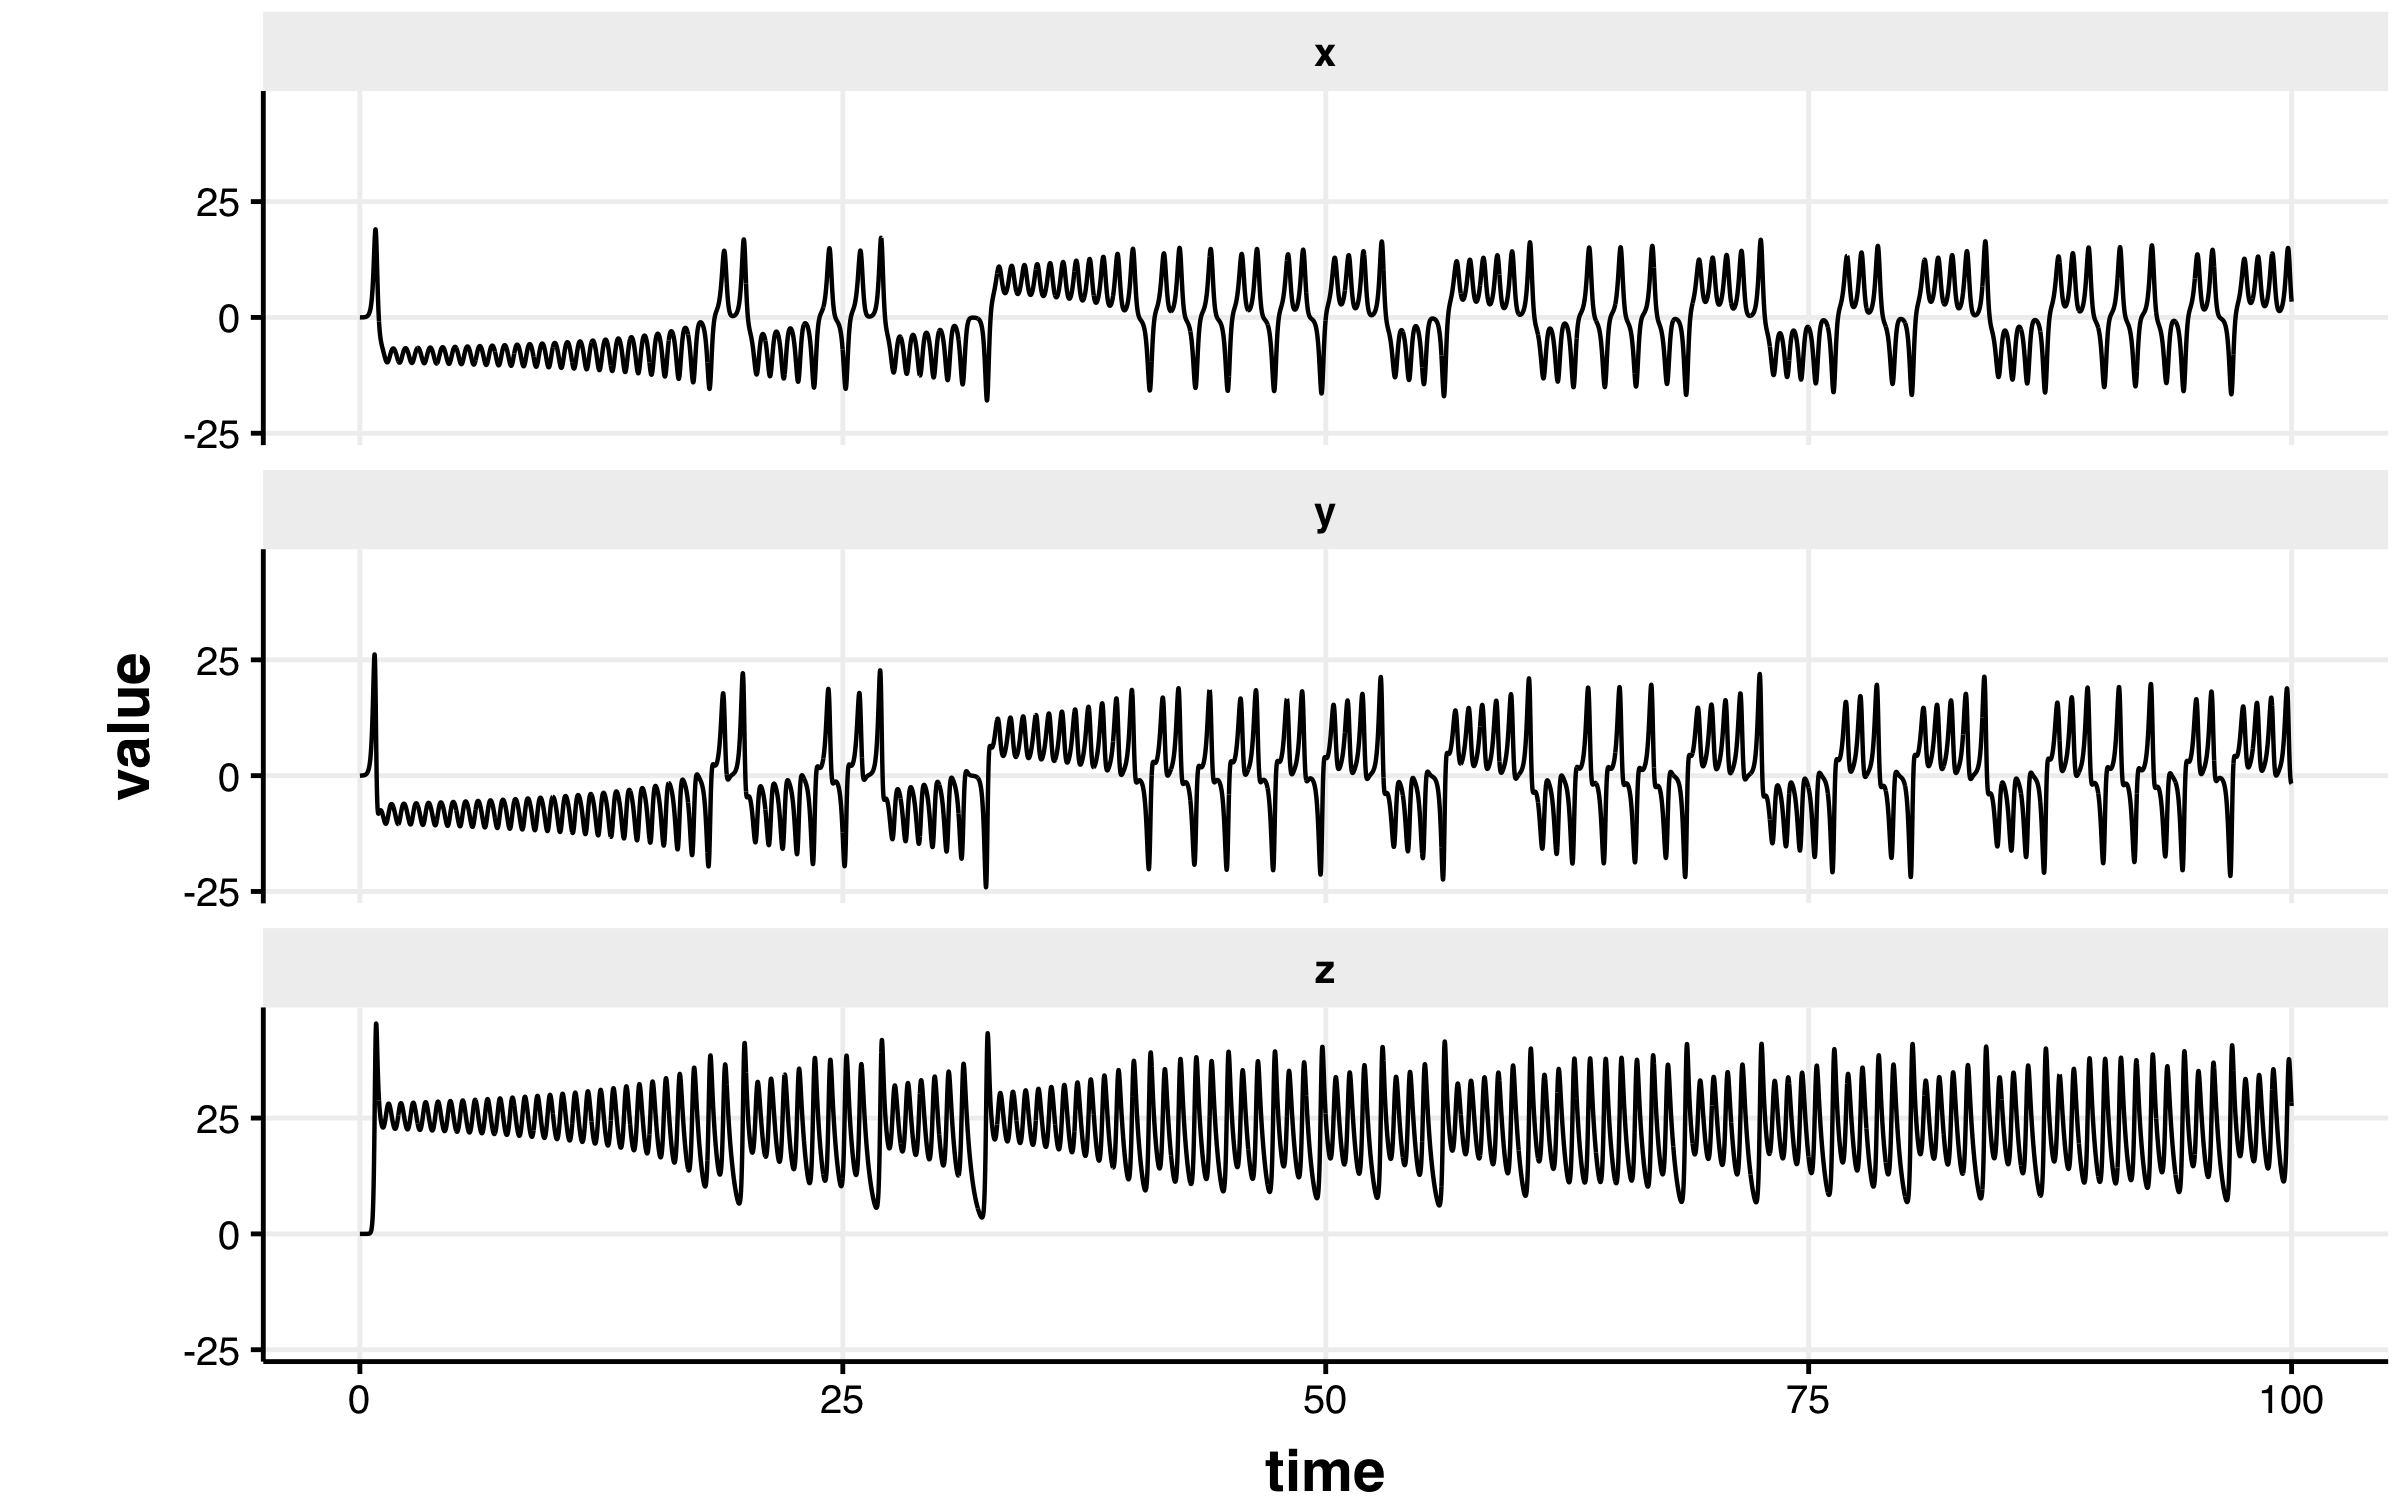
\includegraphics[width=0.55\linewidth]{E:/GitHub/myDissertation/chapterFiles/velocity/figsCalledInDiss/lorenz3D_timeseries} 

}

\caption{An example solution of the Lorenz ('butterfly') represented in individual system compoents.}\label{fig:lorenz3Dts}
\end{figure}

A classic example of state-switching by a system is demonstrated in the
Lorenz (`butterfly') attractor {[}Fig.
\textbackslash{}@ref(fig:lorenz3D); @takens1981detecting{]}. This phase
plot (Fig. @ref(fig:lorenz3D)) provides an informative visual of the
behavior of a chaotic system manifesting two attractors. Although the
periodic, attractor behaviors are made clear when examining the time
series of each dimension (Fig @ref(fig:lorenz3Dts)), identifying such
behaviors in additional dimensions becomes increasingly difficult.

System behavior/trajectory in phase space are used often in dynamical
systems theory and systems ecology to make inference regarding system
behavior and dynamics, but phase space (trajectory) dynamics are not
commonly applied outside theoretical studies as a tool for ecological
data analysis {[}c.f. @sugihara2012detecting for an example of
phase-space reconstruction using Taken's theorem of ecological time
series{]}. Some methods of attractor reconstruction have been applied to
environmental data {[}e.g., individual time series of fisheries stocks,
climate, stock market; @sugihara2012detecting; @ye2015equation{]}, yet
they \textbf{do not incorporate the dynamics of whole-systems}.
Model-free methods for exploring and describing the dynamics of whole
(i.e.~\(>1\) variable) ecological systems are restricted to the
commonly-applied dimnesion reduction techniques and clustering
algorithms (e.g., Principal Components Analysis, K-means clustering). In
fact, this is true of many abrupt change and regime shift indicators.

\hypertarget{rate-of-change-as-an-indicator-of-abrupt-change-in-the-system-trajectory}{%
\subsubsection{Rate of change as an indicator of abrupt change in the
system
trajectory}\label{rate-of-change-as-an-indicator-of-abrupt-change-in-the-system-trajectory}}

How quickly a system switches states {[}e.g., moving from attractor to
another; @ref(fig:lorenz3D){]} may yield insights into the responses of
ecological systems to perturbations (e.g., anthropogenically induced
pressures such as climate change, urbanization) and community shifts
(e.g., species introductions or extinctions, shifts in dominance). For
example, @beck\_variance\_2018 tracked rate of change using chord
distances---a data transformation for positive values and which is
suitable prior to ordination analysis---to capture abrupt changes in
community composition of a temperate, paleodiatom community. Chord
distance, however, is greatest when the observations among data rows
(e.g., time, location) have no species in common. In other words, this
measurement may be most useful in high community turnover conditions.
Identifying alternative numerical methods for estimating system rates of
change may be when the system does not exhibit, for example, high
degrees of turnover.

Rate of change (ROC, often represented as \(\Delta\)) is a term used for
various measures which describe the relationship among to variables,
measuring the change in one variable relative to another. As a refresher
ROC is represented as \textbf{speed} (\(\textbf{S}\)) or
\textbf{velocity} (\(\textbf{V}\)), where (\(\textbf{S}\)) is the
adirectional magnitude (i.e.~it is a scalar) of the displacement of an
object over unit time and \(\textbf{V}\) describes both the direction
and magnitude (i.e.~it is a vector) of the object's movement in
spacetime. \(\textbf{S}\) is a scalar taking values of \(\geq0\) and
\(\textbf{V}\) can take any value between \(-\infty\) and \(\infty\).
For example, consider a car travelling at a constant speed of
\(50\frac{km}{h}\) around along a hilly landscape, where it is ascending
and descending hills. Although \(\textbf{S}\) is constant,
\(\textbf{V}\) changes in a sunusoidal fashion, where \(\textbf{V}\) is
\(\textbf{V}>0\) when ascending, \(\textbf{V}<0\) when descending, and
\(\textbf{V}\approx0\) at in the valleys and at the peaks of the hills.
Although \(\textbf{S}\) is useful when estimating other scalar
quantities (e.g., \(\frac{miles}{gallon}\)), given a starting and/or
final position in space, \(\textbf{S}\) is not informative of its the
path travelled.

\hypertarget{aims}{%
\subsubsection{Aims}\label{aims}}

Here, I propose a method which simply describes the rate of change
behavior of system dynamics in phase space: \textbf{velocity}, \(V\). An
alternative to other complicated, model-free approaches {[}e.g., Fisher
Information; @cabezas\_towards\_2002{]}, the velocity metric allows one
to examine the behavior of an entire system along its trajectory
(through space or time) without having to reconstruct the pahse space.
The ability to handle noisy and high-dimensional data and the lack of
subjective parameters in calculating the metric makes this method an
ideal alternative to existing early warning indicators and phase-space
reconstruction methods.

I first describe the steps for calculating this new metric (\(v\)), as
both a dimension reduction technique and abrupt change indicator.
Although this is the first instance of this calculation to, alone, be
suggested as a regime detection metric, it has been used as part of a
larger series of calculations of the Fisher Information metric {[}see
Ch. @ref(fiGuide){]}, first introduced in @fath\_regime\_2003. I use
this theoretical system to present baseline estimates of the expected
behavior of \(v\) under various scenarios of changing mean and
variability in a theoretical, discussing the contexts under which this
metric may signal abrupt changes. Finally, I explore the utility of this
metric in identifying known regime shifts in an empirical
paleoecological time series data.

\hypertarget{analytical-approach}{%
\subsubsection{Analytical approach}\label{analytical-approach}}

I first describe the steps for calculating velocity by constructing a
simple, two-variable system which exhibits only a rapid, discontinuous
change in the means of the state variables. I next vary the mean and
variance of the state variables of this system to demonstrate baseline
expectations for the behavior of velocity under a simple rapid shift
scenario. Next, I construct a second model system similar to the first,
but one which exhibits a non-discontinuous rapid change in the state
variables. The purpose of this section is three-fold. First, I
demonstrate how velocity behaves when the system undergoes varying
degrees of change (e.g., slow change versus nearly discontinuous,
rapid). Second, I concurrently identify baseline expectations of
velocity under varying conditions of mean and variability of the state
varilbes before and after a shift. Third, by introducing a smoothing
function to the rapid shift, we gain an understanding of how process
variability (noise) impacts the shift detectability by the velocity
metric. Finally, I calculate the velocity of an empirical, paleolitic
freshwater diatom community time series to demonstrate the utility of
the velocity metric in highly noisy, high dimensional, and
irregularly-sampled data.

\hypertarget{steps-for-calculating-velocity-v}{%
\subsection{\texorpdfstring{Steps for Calculating velocity,
\(v\)}{Steps for Calculating velocity, v}}\label{steps-for-calculating-velocity-v}}

In this section, I first demonstrate the calculations of velocity using
a very simple, two-variable toy system. The first system exhibits a
rapid shift at a single point in time, where mean and variance are
constant before and after the shift point. I demonstrate the signals
achieved with and the variability within the \(v\) calculation by
exploring a number of scenarios of this simple system. For the examples
in this section, observations of \(x_i\) are randomly drawn from
distribution \(x_i\sim Normal(\mu, \sigma)\), where \(\mu\) is the mean
and \(\sigma\) is the standard deviation.

\begin{figure}

{\centering 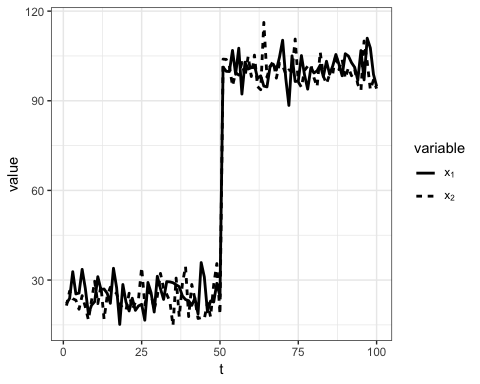
\includegraphics[width=0.65\linewidth]{06-chap-velocity_files/figure-latex/sysEx-1} 

}

\caption{The 2-variable discrete time toy system used to demonstrate steps for calculating system velocity. Each variable, $x$, is drawn from a normal distribution with means that change at $t = 50$. State variables have constant standard deviation, $\sigma = 5$.}\label{fig:sysEx}
\end{figure}

Consider a system (Fig. @ref(fig:sysEx)) with \(N\) state variables
(\(x_i\)), with observations taken at time points, \(t\). System
velocity is calculated as the cumulative sum over time period \(t_0\) to
\(t_j\), as the total change in all state variables, \{\(x_1 ...x_N\)\},
between two adjacent time points, e.g., \(t_j\) and \(t_{j+1}\), denoted
\(t_{j,j+1}\). I use this simple, two-variable system to demonstrate how
\emph{velocity} is calculated. The system comprises variables \(x_1\)
and \(x_2\), with observations occurring at each time point
\(t = {1,2,3,...100}\). First, we calculate the change in each state
variable, \(x_i\), between two adjacent points in time, \(t_j\) and
\(t_{j+1}\), such that the difference, \(x_{t_{j+1}} - x_{t_j}\) is
assigned to the latter time point, \(t_{j+1}\). For example, in our toy
data, we use observations at time points \(t = 1\) \& \(t=2\) (Fig.
@ref(fig:sysEx2)). For all examples in this chapter, the state variables
\(x_1\) and \(x_2\) were drawn from a normal distribution (using
function \emph{rnorm}), with parameters \(\bar{x}_i\) (mean) and
\(\sigma_i\) (sd) for 100 time steps, \(t\). The regime shift in this
system occurs at \(t=50\), where a shift in either or both \(\bar{x}_i\)
or \(\sigma_i\).

\begin{figure}

{\centering 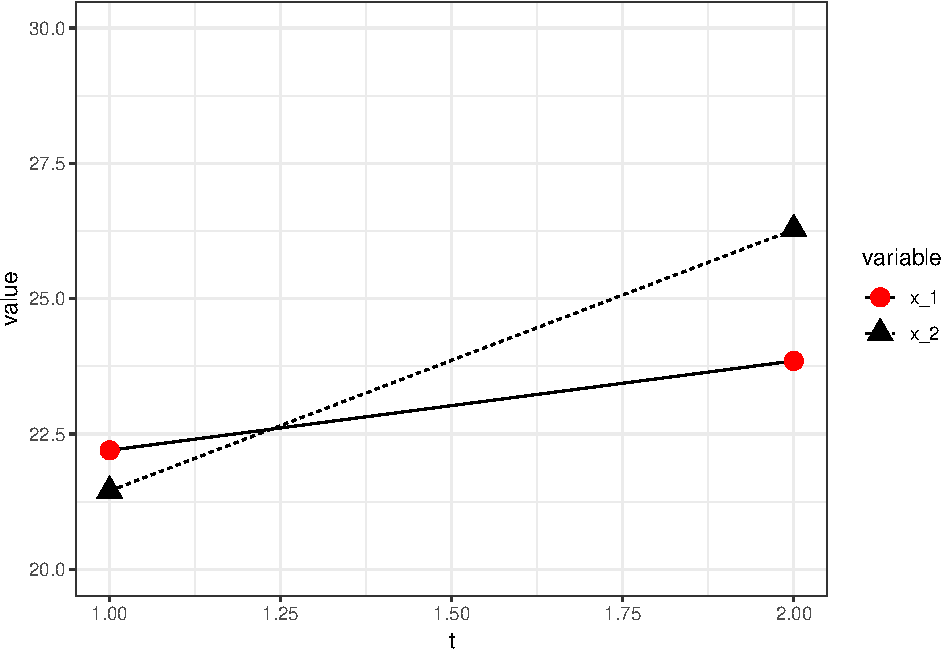
\includegraphics[width=0.65\linewidth]{06-chap-velocity_files/figure-latex/sysEx2-1} 

}

\caption{Data used to calculate velocity at the first two time points, $t_1$ and $t_2$.}\label{fig:sysEx2}
\end{figure}

\hypertarget{steps-for-calculating-v}{%
\subsubsection{\texorpdfstring{Steps for calculating
\(v\)}{Steps for calculating v}}\label{steps-for-calculating-v}}

\hypertarget{step-1-calculate-delta-x_i}{%
\paragraph{\texorpdfstring{Step 1: Calculate
\(\Delta x_i\)}{Step 1: Calculate \textbackslash{}Delta x\_i}}\label{step-1-calculate-delta-x_i}}

The first step is to calculate the change in values for each state
variables, \(x_i\), between two consecutive time points {[}e.g., from
time \(t\) to \(t+1\) for the discrete-time system; Fig.
@ref(fig:sysEx2); Eq. @ref(eq:diffX){]}: \begin{equation}
\Delta x_i = x_{i(t+1)} - x_{it} 
(\#eq:diffX)
\end{equation}

Note that \(\Delta x_i\) can take any value between \(-\infty\) and
\(\infty\).

\hypertarget{step-2-calculate-distance-travelled-s}{%
\paragraph{\texorpdfstring{Step 2: Calculate distance travelled,
\(s\)}{Step 2: Calculate distance travelled, s}}\label{step-2-calculate-distance-travelled-s}}

Next, we calculate the total change in the multivariable system as a
function of the change in all state variables \(x_i\). First, we
calculate \(\Delta s\) as the square root of the sum of squares of the
changes in all state variables per Pythagora's theorem (Eq.
@ref(eq:ds)): \begin{equation}
\Delta s = \sqrt{\sum{\Delta x_i^2}}
(\#eq:ds)
\end{equation}

Although \(\Delta s\) represents the absolute change in the system
between consecutive points in time, this measure is not yet relative
along the system's trajectory. To create a relative value we next
calculate the total distance travelled along the system trajectory,
\(s\), as the cumulative sum of \(\Delta s\) (Eq. @ref(eq:ds)) since the
first observation, such that a cumulative sum is calculated for every
\(t\) over the interval \([0,T]\) (Eq. @ref(eq:s)):

\begin{equation}
s_T = \Sigma_{t=0}^{T}{\Delta s}) 
  (\#eq:s)
\end{equation}

\begin{figure}

{\centering 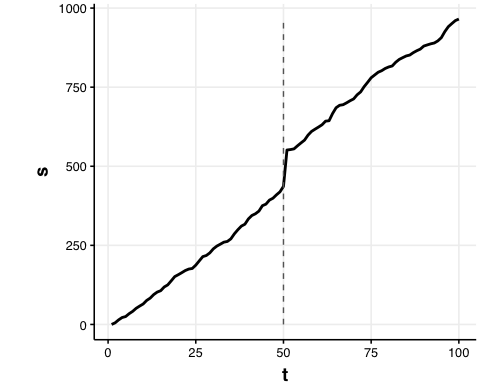
\includegraphics[width=0.65\linewidth]{06-chap-velocity_files/figure-latex/sysExs-1} 

}

\caption{Distance travelled, $s$, for the 2-species toy system.}\label{fig:sysExs}
\end{figure}

We now have a single measure, \(s_T\) {[}hereafter referred to as \(s\);
Eq. @ref(eq:s){]} at each discrete point in time in our
\(N\)-dimensional system (Fig. @ref(fig:sysExs)). It should be noted
that \(s\)(Fig. @ref(fig:sysExs)) is monotonically increasing since the
value of \(\Delta s\) (Eq. @ref(eq:ds)) is a sum of squares. Although
discussed in a later section, it is important to note that \(s\) is not
unitless---that is, \(s\) has units of the state variables, \(x_i\). For
example, if our 2-variable toy system represents biomass, then the units
of \(s\) represents the cumulative absolute change in biomass of the
entire system.

\hypertarget{step-3-calculate-velocity-v-or-fracdelta-sdelta-t}{%
\paragraph{\texorpdfstring{Step 3: Calculate velocity, \(v\) (or
\(\frac{\Delta s}{\Delta t}\))}{Step 3: Calculate velocity, v (or \textbackslash{}frac\{\textbackslash{}Delta s\}\{\textbackslash{}Delta t\})}}\label{step-3-calculate-velocity-v-or-fracdelta-sdelta-t}}

Finally, we calculate the \textbf{system velocity}, \(v\) (or
\(\frac{\Delta s}{\Delta t}\)), by first calculating the change in \(s\)
(Eq. @ref(eq:s)), and then divide by the total time elapsed between
consecutive sampling points: \begin{equation}
 v = \frac {s_{t+1}-s_{t}}{\Delta t} 
(\#eq:velocity)
\end{equation}

\begin{figure}

{\centering 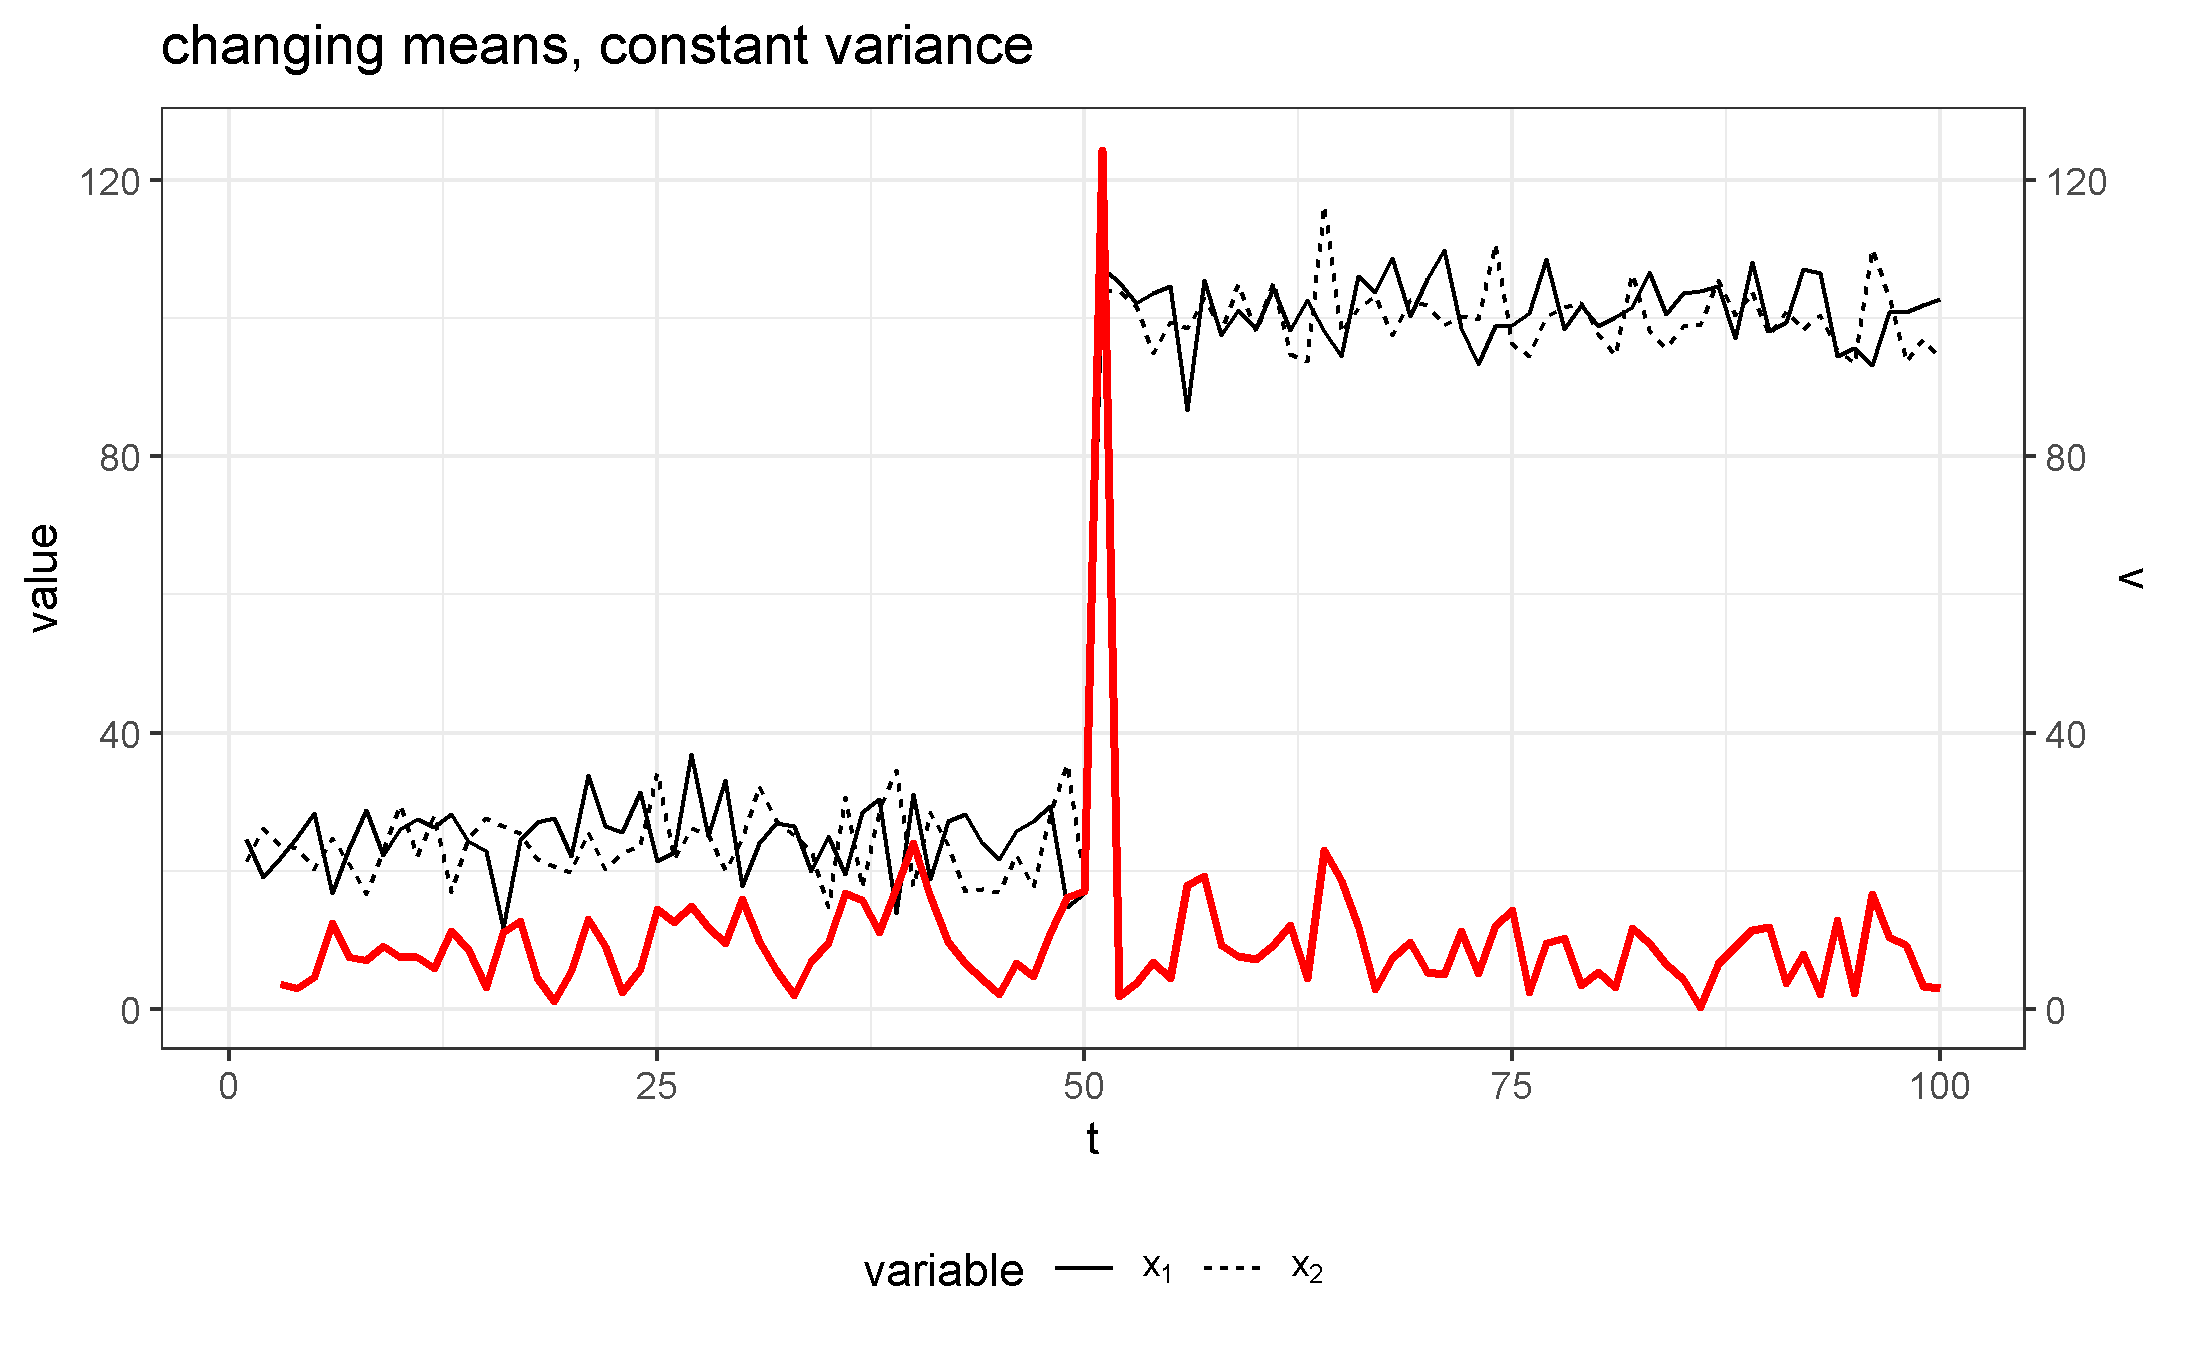
\includegraphics[width=0.65\linewidth]{E:/GitHub/myDissertation/chapterFiles/velocity/figsCalledInDiss/velocitySysEx1} 

}

\caption{System change ($s$) and velocity ($v$) of the model system over the time period. Constant means ($\bar{x}_{pre}=25$, $\bar{x}_{post}=10$) and sharp change in variance for both state variables, $\sigma =5$.}\label{fig:velocSysEx1}
\end{figure}

\begin{table}[t]

\caption{\label{tab:distTab}Steps outlined for calculating system velocity, $v$, using the 2-variable toy data as an example.}
\centering
\begin{tabular}{ccccccccc}
\toprule
t & $x_1$ & $x_2$ & $\Delta x_1$ & $\Delta x_2$ & $\Delta t$ & $\sqrt(\sum_{i=1}^N \Delta x_i^2) $ & $s$ & $v$\\
\midrule
1 & 22.198 & 21.448 &  &  &  &  &  & \\
2 & 23.849 & 26.284 & 1.651 & 4.836 & 1 & 5.111 & 5.111 & \\
3 & 32.794 & 23.767 & 8.944 & -2.518 & 1 & 9.292 & 14.403 & 9.292\\
4 & 25.353 & 23.262 & -7.441 & -0.504 & 1 & 7.458 & 21.861 & 7.458\\
5 & 25.646 & 20.242 & 0.294 & -3.020 & 1 & 3.035 & 24.895 & 3.035\\
\bottomrule
\end{tabular}
\end{table}

The numerical results for each step in the calculation of velocity
{[}Eq. @ref(eq:velocity){]} is demonstrated using the first five time
points of our toy system (Fig. @ref(fig:sysEx)) in Table
@ref(tab:distTab).

\hypertarget{velocity-v-performance-under-a-discontinuous-transition}{%
\subsection{\texorpdfstring{Velocity \emph{v} performance under a
discontinuous
transition}{Velocity v performance under a discontinuous transition}}\label{velocity-v-performance-under-a-discontinuous-transition}}

I used simulation techniques to determine the baseline expectations of
the performance of velocity \(v\) under varying degrees of rapid shifts
in the mean and variance of the toy system. The toy system in this
section undergoes a discontinuous shift at \(t = 50\) (see
@ref(Fig:sysEx)). If the system undergoes a rapid and discontinuous
change in one or more state variables, the velocity, beacuse it is a
rate of change, may \(\rightarrow \infty\) as
\(\Delta t \rightarrow 0\). Therefore, it is important to understand the
degree to which

, while varying two each of the following system parameters at the
regime shift: - \(\bar{x}_1\), increase in the mean value of \(x_1\) at
\(t=50\)\\
- \(\sigma_1\), change in variance of \(x_1\) at \(t=50\)

Simulations consisted of 10,000 random samples drawn from the normal
distribution for each paramter, I randomly drew the toy system samples
10,000 times under increasing values of \(\bar{x}_1\) and \(\sigma_1\).
To identify patterns in the influence of paramter values on velocity, I
present the mean values of \(v\) across all simulations, with confidence
intervals of \(\pm 2\) standard deviations. As mentioned above, the
state variables \(x_1\) and \(x_2\) were drawn from a normal
distribution (using function \emph{rnorm}), with parameters
\(\bar{x}_i\) (mean) and \(\sigma_i\) (sd) for 50 time steps, \(t\).

\hypertarget{velocity-under-varying-degrees-of-varying-post-shift-mean}{%
\paragraph{Velocity under varying degrees of Varying post-shift
mean}\label{velocity-under-varying-degrees-of-varying-post-shift-mean}}

I examined the influence of the magnitude of change in \(x_1\) in the
period before (pre; \(t <50\)) and after (post; \(t \geq 50\)) by
varying the mean parameter, \(\bar{x}_1\) in the set
\(W=\{25,30,35,...100 \}\) (Figs. @ref(fig:simVplot1),@ref(simVplot2)).
As expected, the magnitude of \(v\) increases linearly as the total
difference between \(\bar{x}_{1_{pre}}\) and \(\bar{x}_{1_{post}}\)
increases (@ref(fig:simVplot2)). This is not surprising because \(s\)
increases as the total change in abundance across the entire sytem
increases (Eq. @ref(eq:s)). Consequently the potential of \(v\) also
increases with total state variable values (e.g.~abundance, biomass).
The linear relationship among \(v\) and total state variable values
indicates that while \(v\) is capable of identifying large shifts in
data structure, it may fail to identify subtle changes (i.e.~lower
effect sizes).

\begin{figure}

{\centering 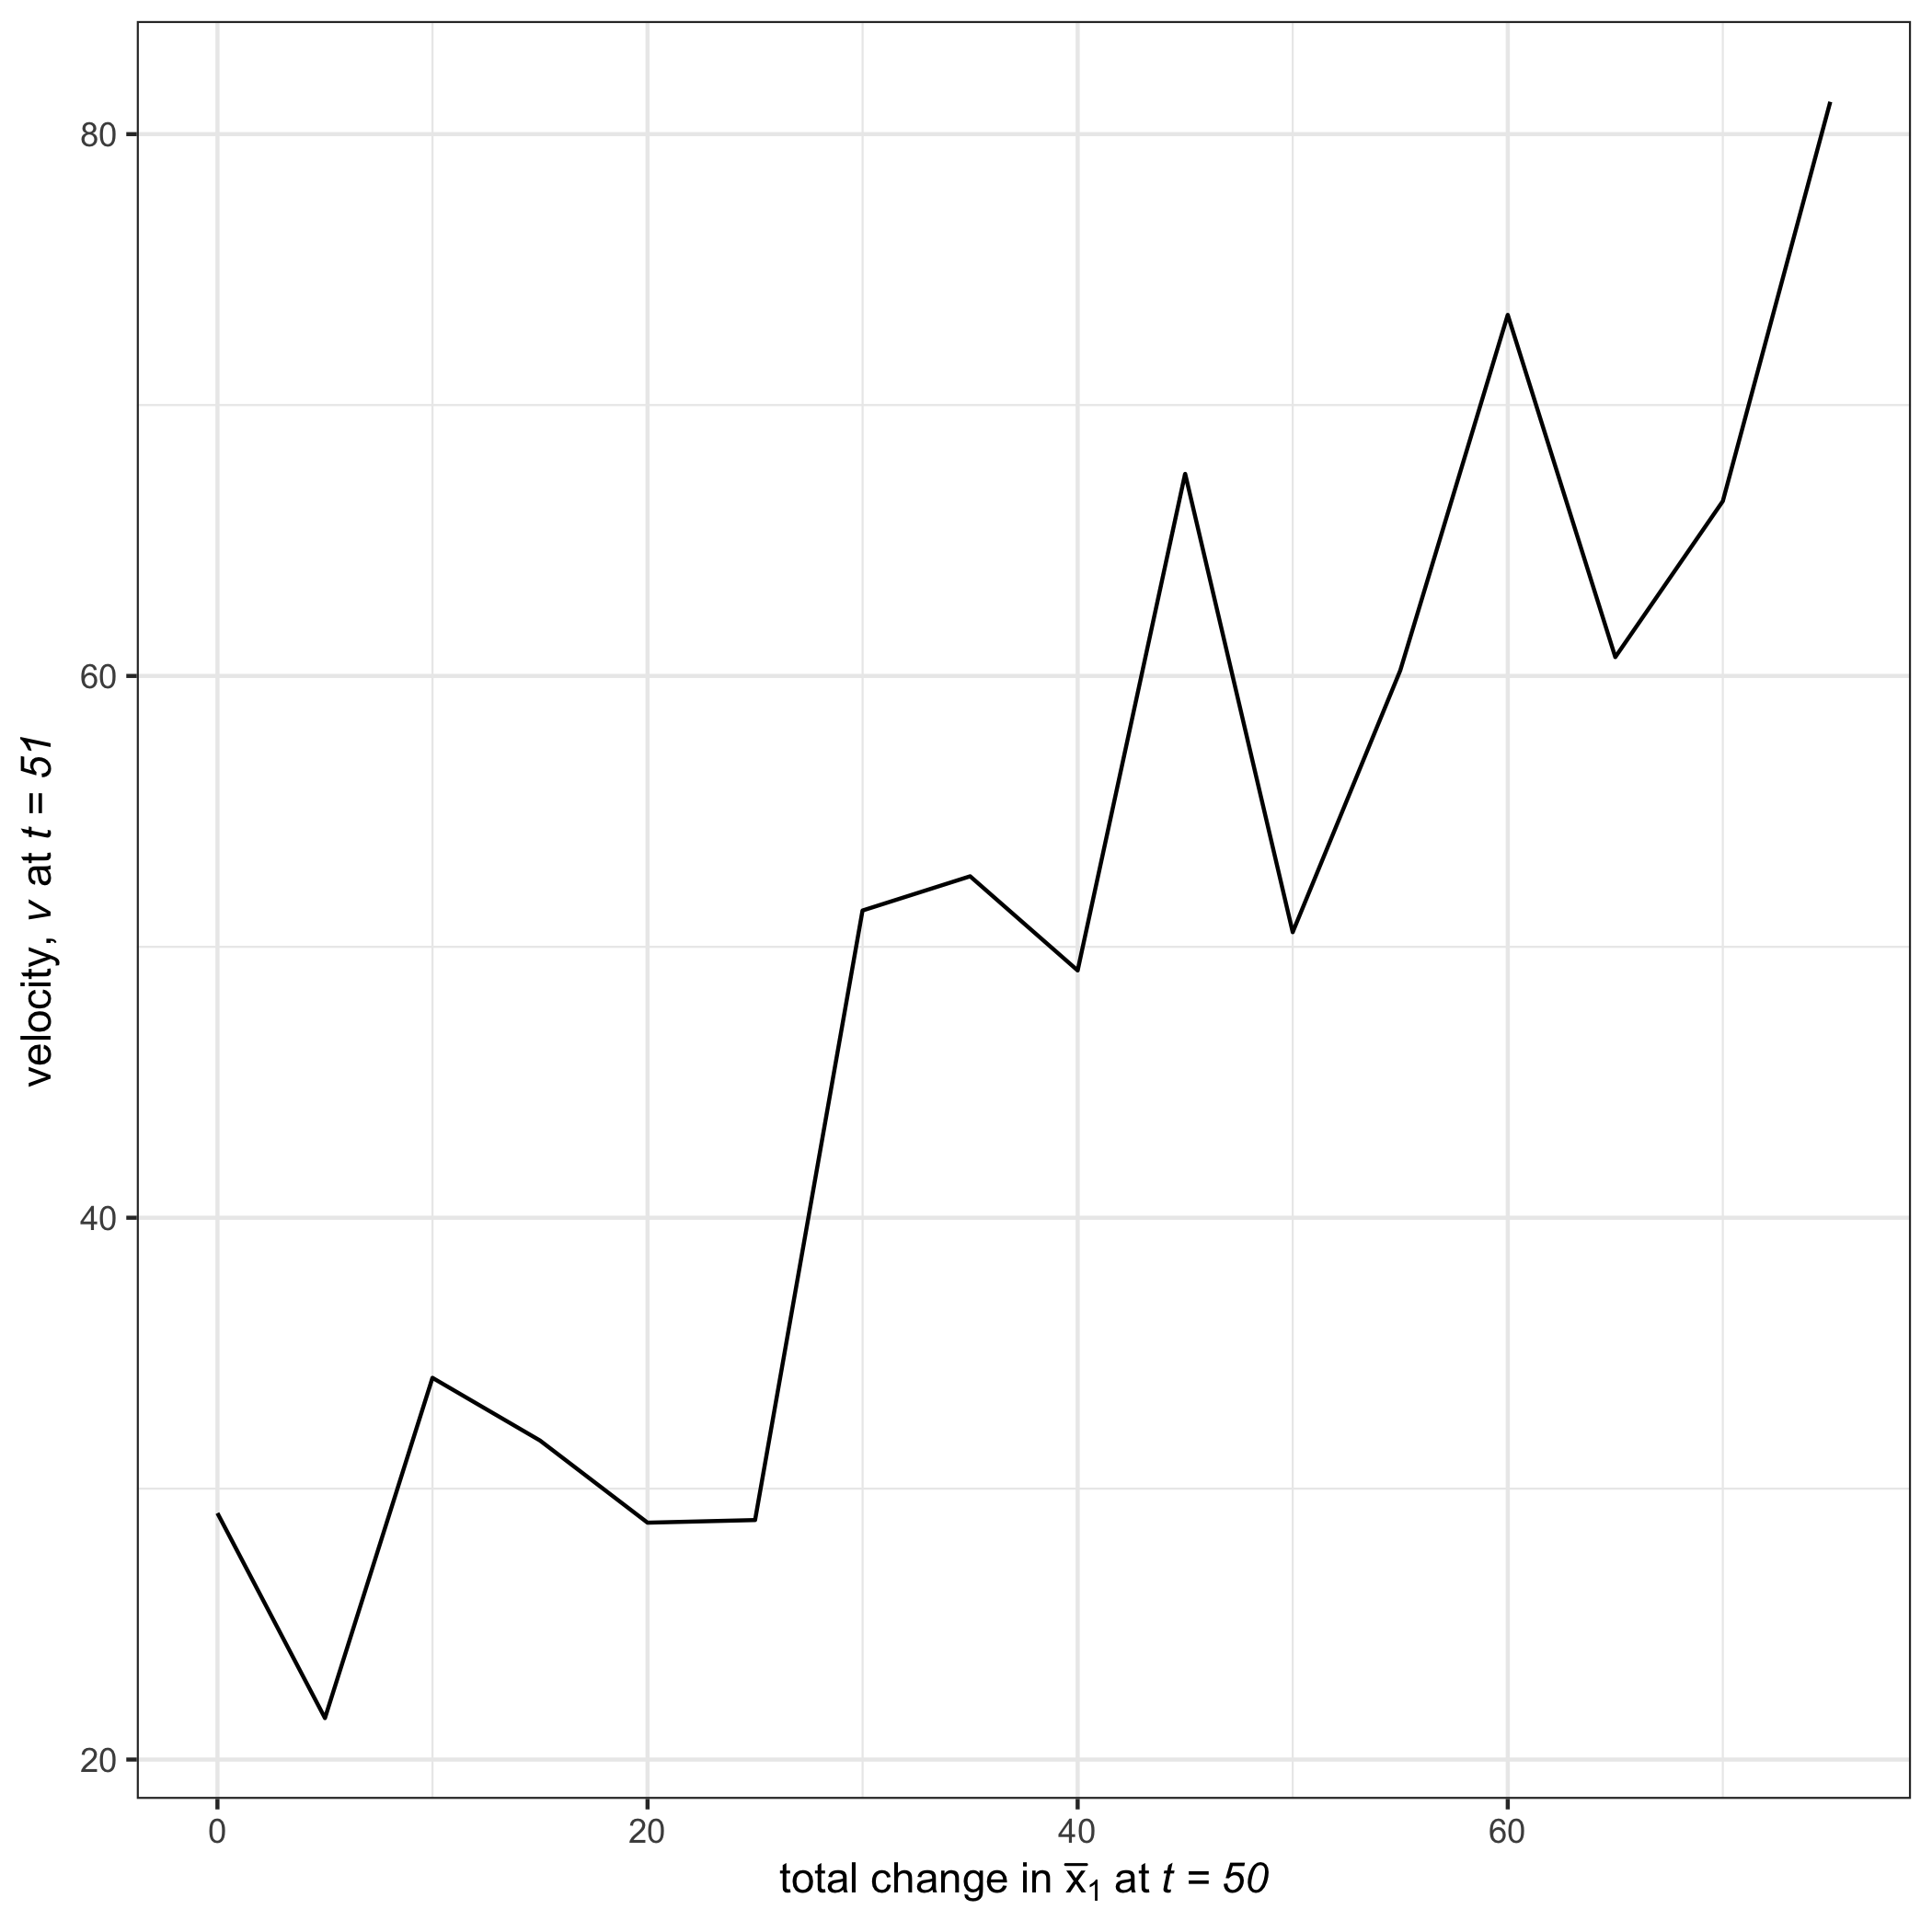
\includegraphics[width=0.55\linewidth]{E:/GitHub/myDissertation/chapterFiles/velocity/figsCalledInDiss/simVplot1} 

}

\caption{Velocity ($v$) generally increases as the total change in the mean value of $\bar{x}_{1_{t=50}}$ increases in a single iteration of our toy system ($N_{iter}=1$, seed = 123). This 2-variable system exhibits a regime shift at $t=50$, where variance is constant $\sigma = 5$, $\bar{x}_1 = 25$ when $t<50$,  $\bar{x}_2=50$ when $t\geq50$, $\bar{x}_1 = 25$ when $t <50$.}\label{fig:simVplot1}
\end{figure}
\begin{figure}

{\centering 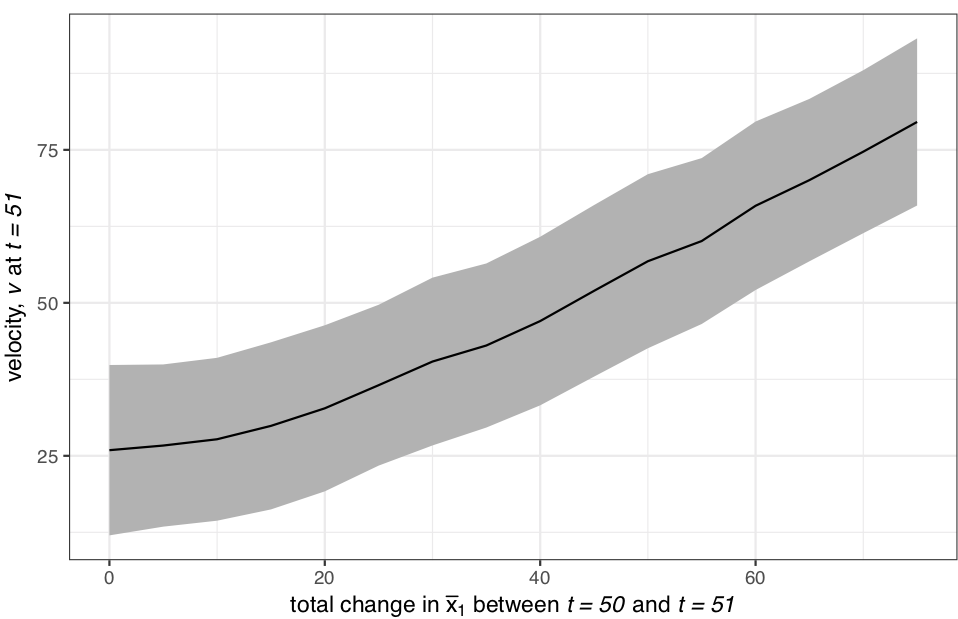
\includegraphics[width=0.55\linewidth]{E:/GitHub/myDissertation/chapterFiles/velocity/figsCalledInDiss/simVplot2} 

}

\caption{Change in velocity ($v$) as the total change in the mean value of $\bar{x}_{2_{t=50}}$ over 10,000 simulations. A regime shift was induced at $t=50$ with constant varoance $\sigma = 5$, $\bar{x}_2 = 25$ when $t<50$,  and changes in variable mean values, $\bar{x}_2 = 50$ when $t \geq 50$, $\bar{x}_1 = 25$ when $t<50$.}\label{fig:simVplot2}
\end{figure}

\hypertarget{varying-post-shift-variance}{%
\paragraph{Varying post-shift
variance}\label{varying-post-shift-variance}}

In the previous example, variance was constant before and after the
abrupt shift at \(t=50\). To determine whether the signal emitted by
\(v\) at the regime shift is lost or dampened when increasing variance I
varied the variance parameter, \(\sigma_1\) along the set
\(W = \{1,2,3,...25 \}\). The variance for both state variables
(\(x_1, x_2\)) prior to the regime shift, \(\sigma_{x_1}\) and
\(\sigma_{x_2}\), was \(5\), with the change occurring in
\(\sigma_{x{_1_{post}}}\).

\begin{figure}

{\centering 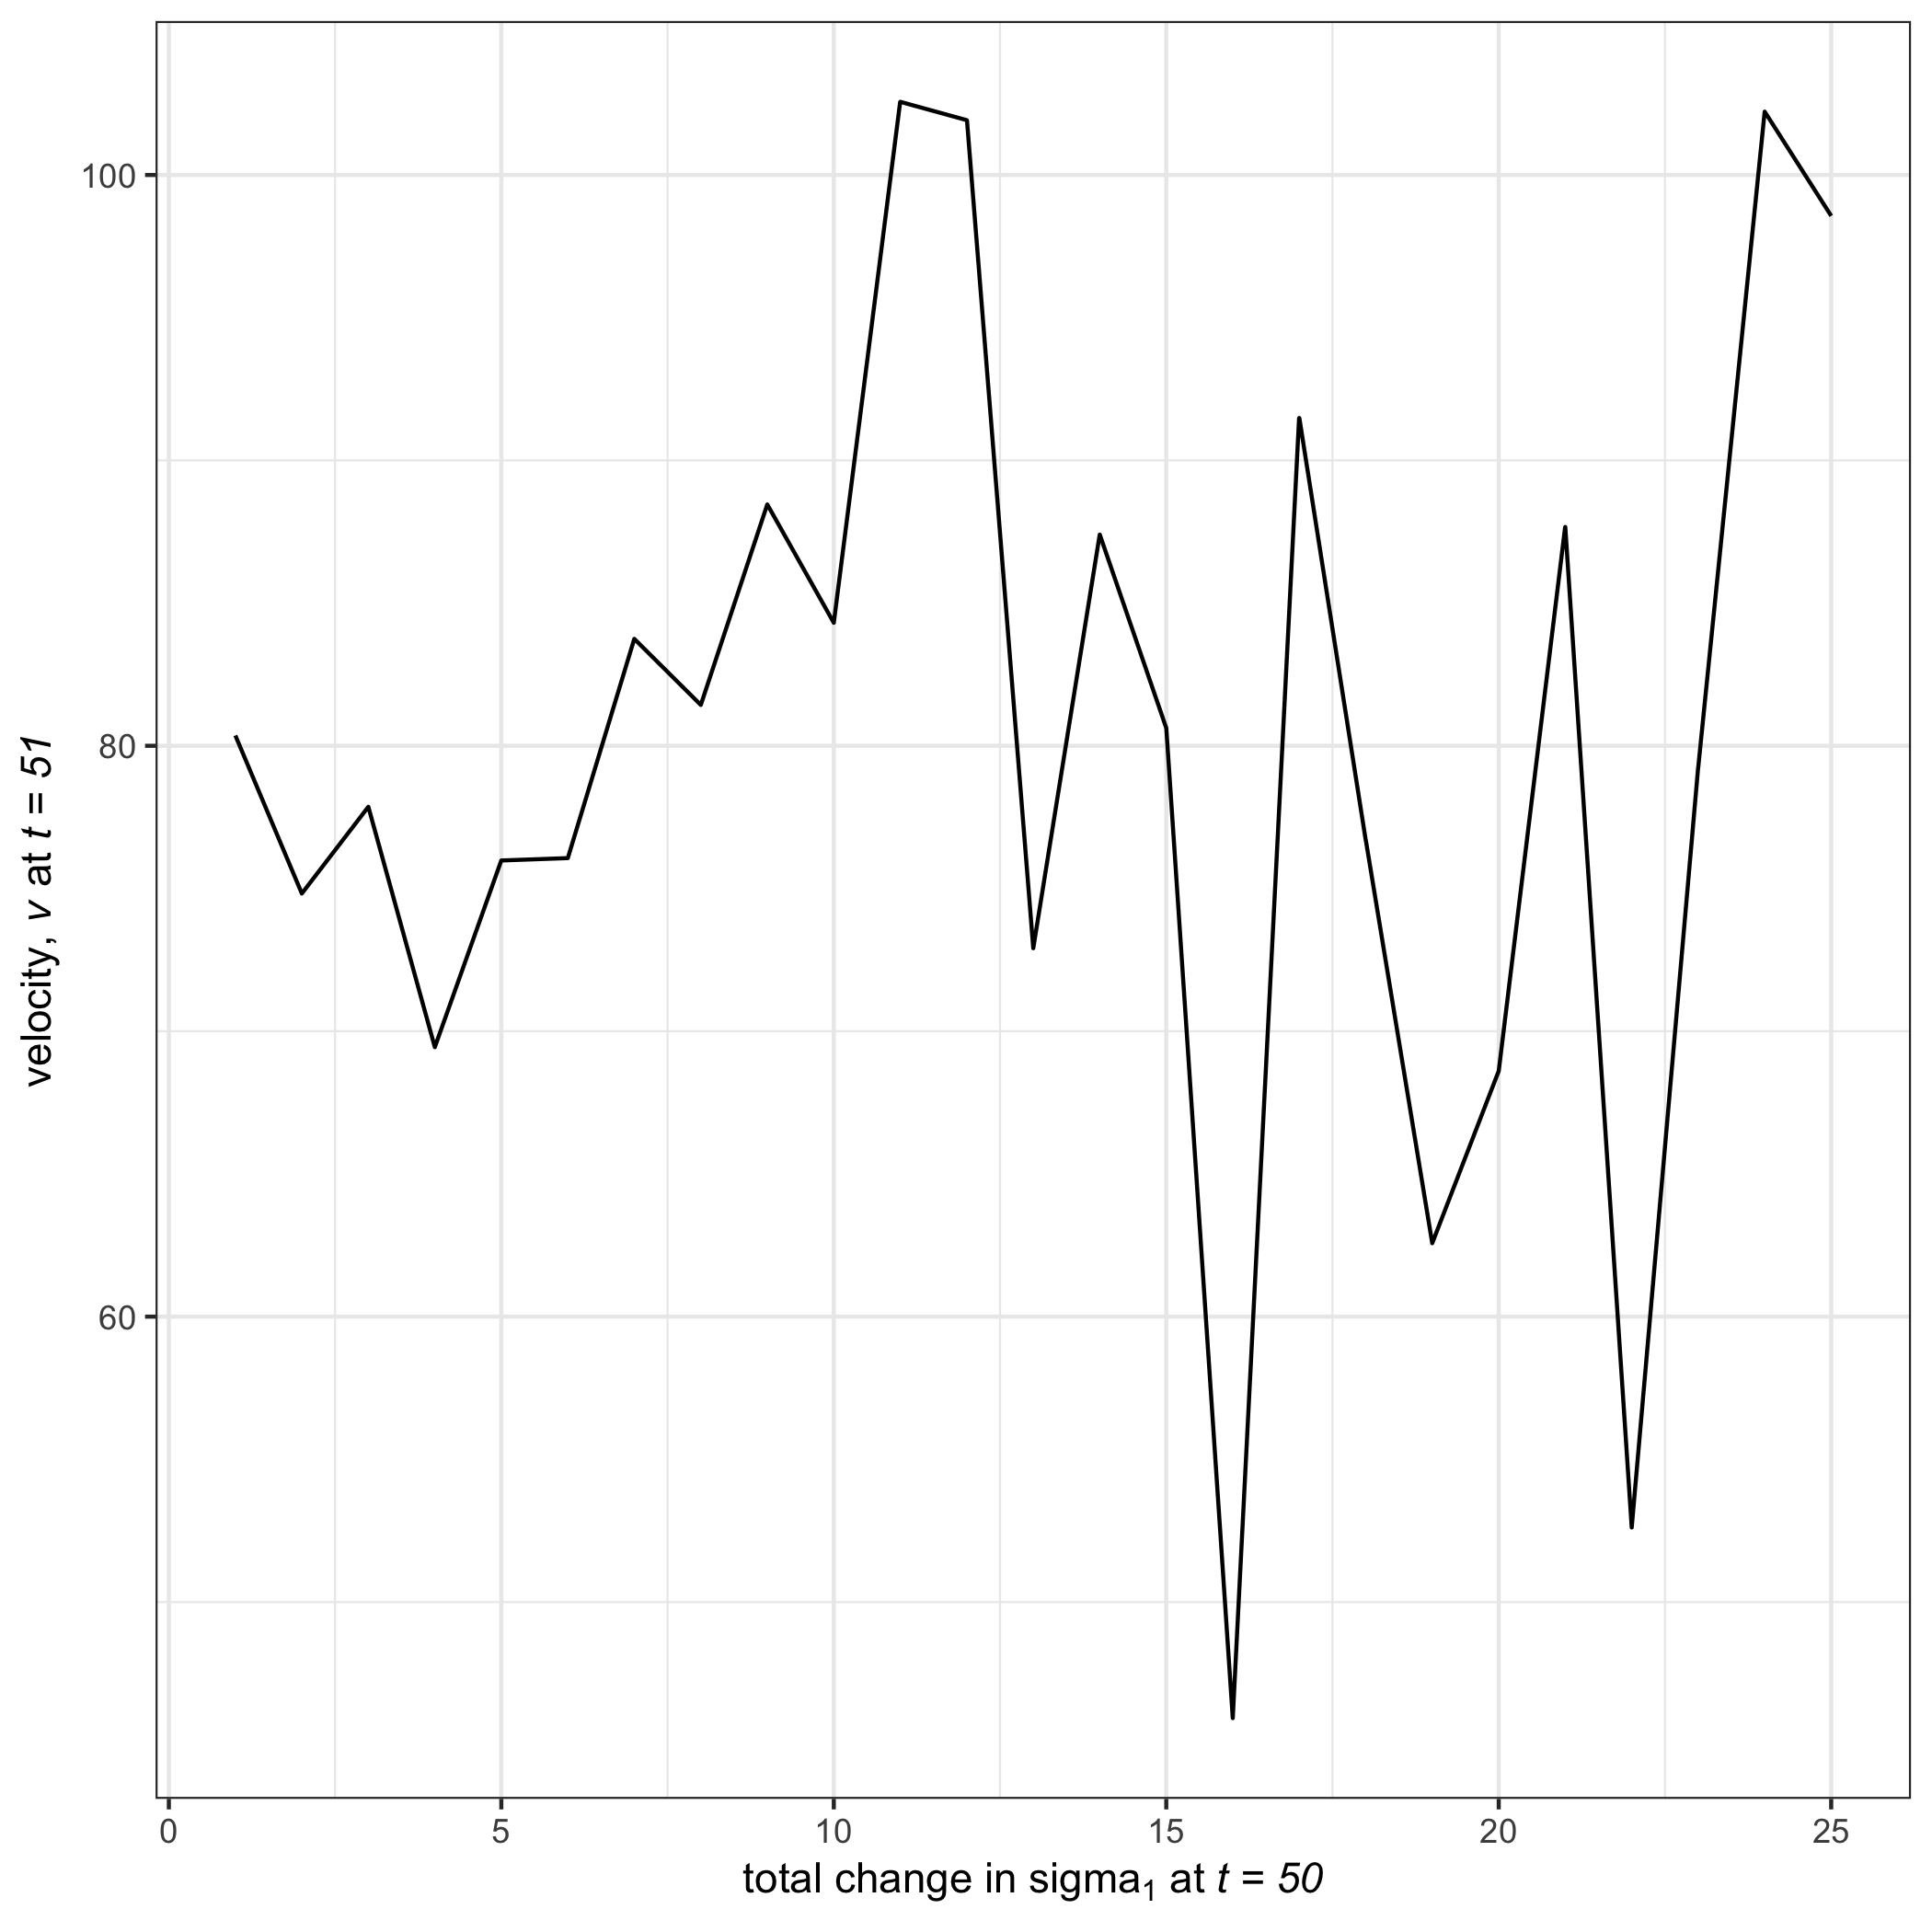
\includegraphics[width=0.65\linewidth]{E:/GitHub/myDissertation/chapterFiles/velocity/figsCalledInDiss/simVarPlot} 

}

\caption{High variance of velocity ($v$) in a single iteration ($N_{iter}=1$, seed = 123) of simulations as we increase $\sigma_1$ at $t=50$.}\label{fig:simVarPlot}
\end{figure}
\begin{figure}

{\centering 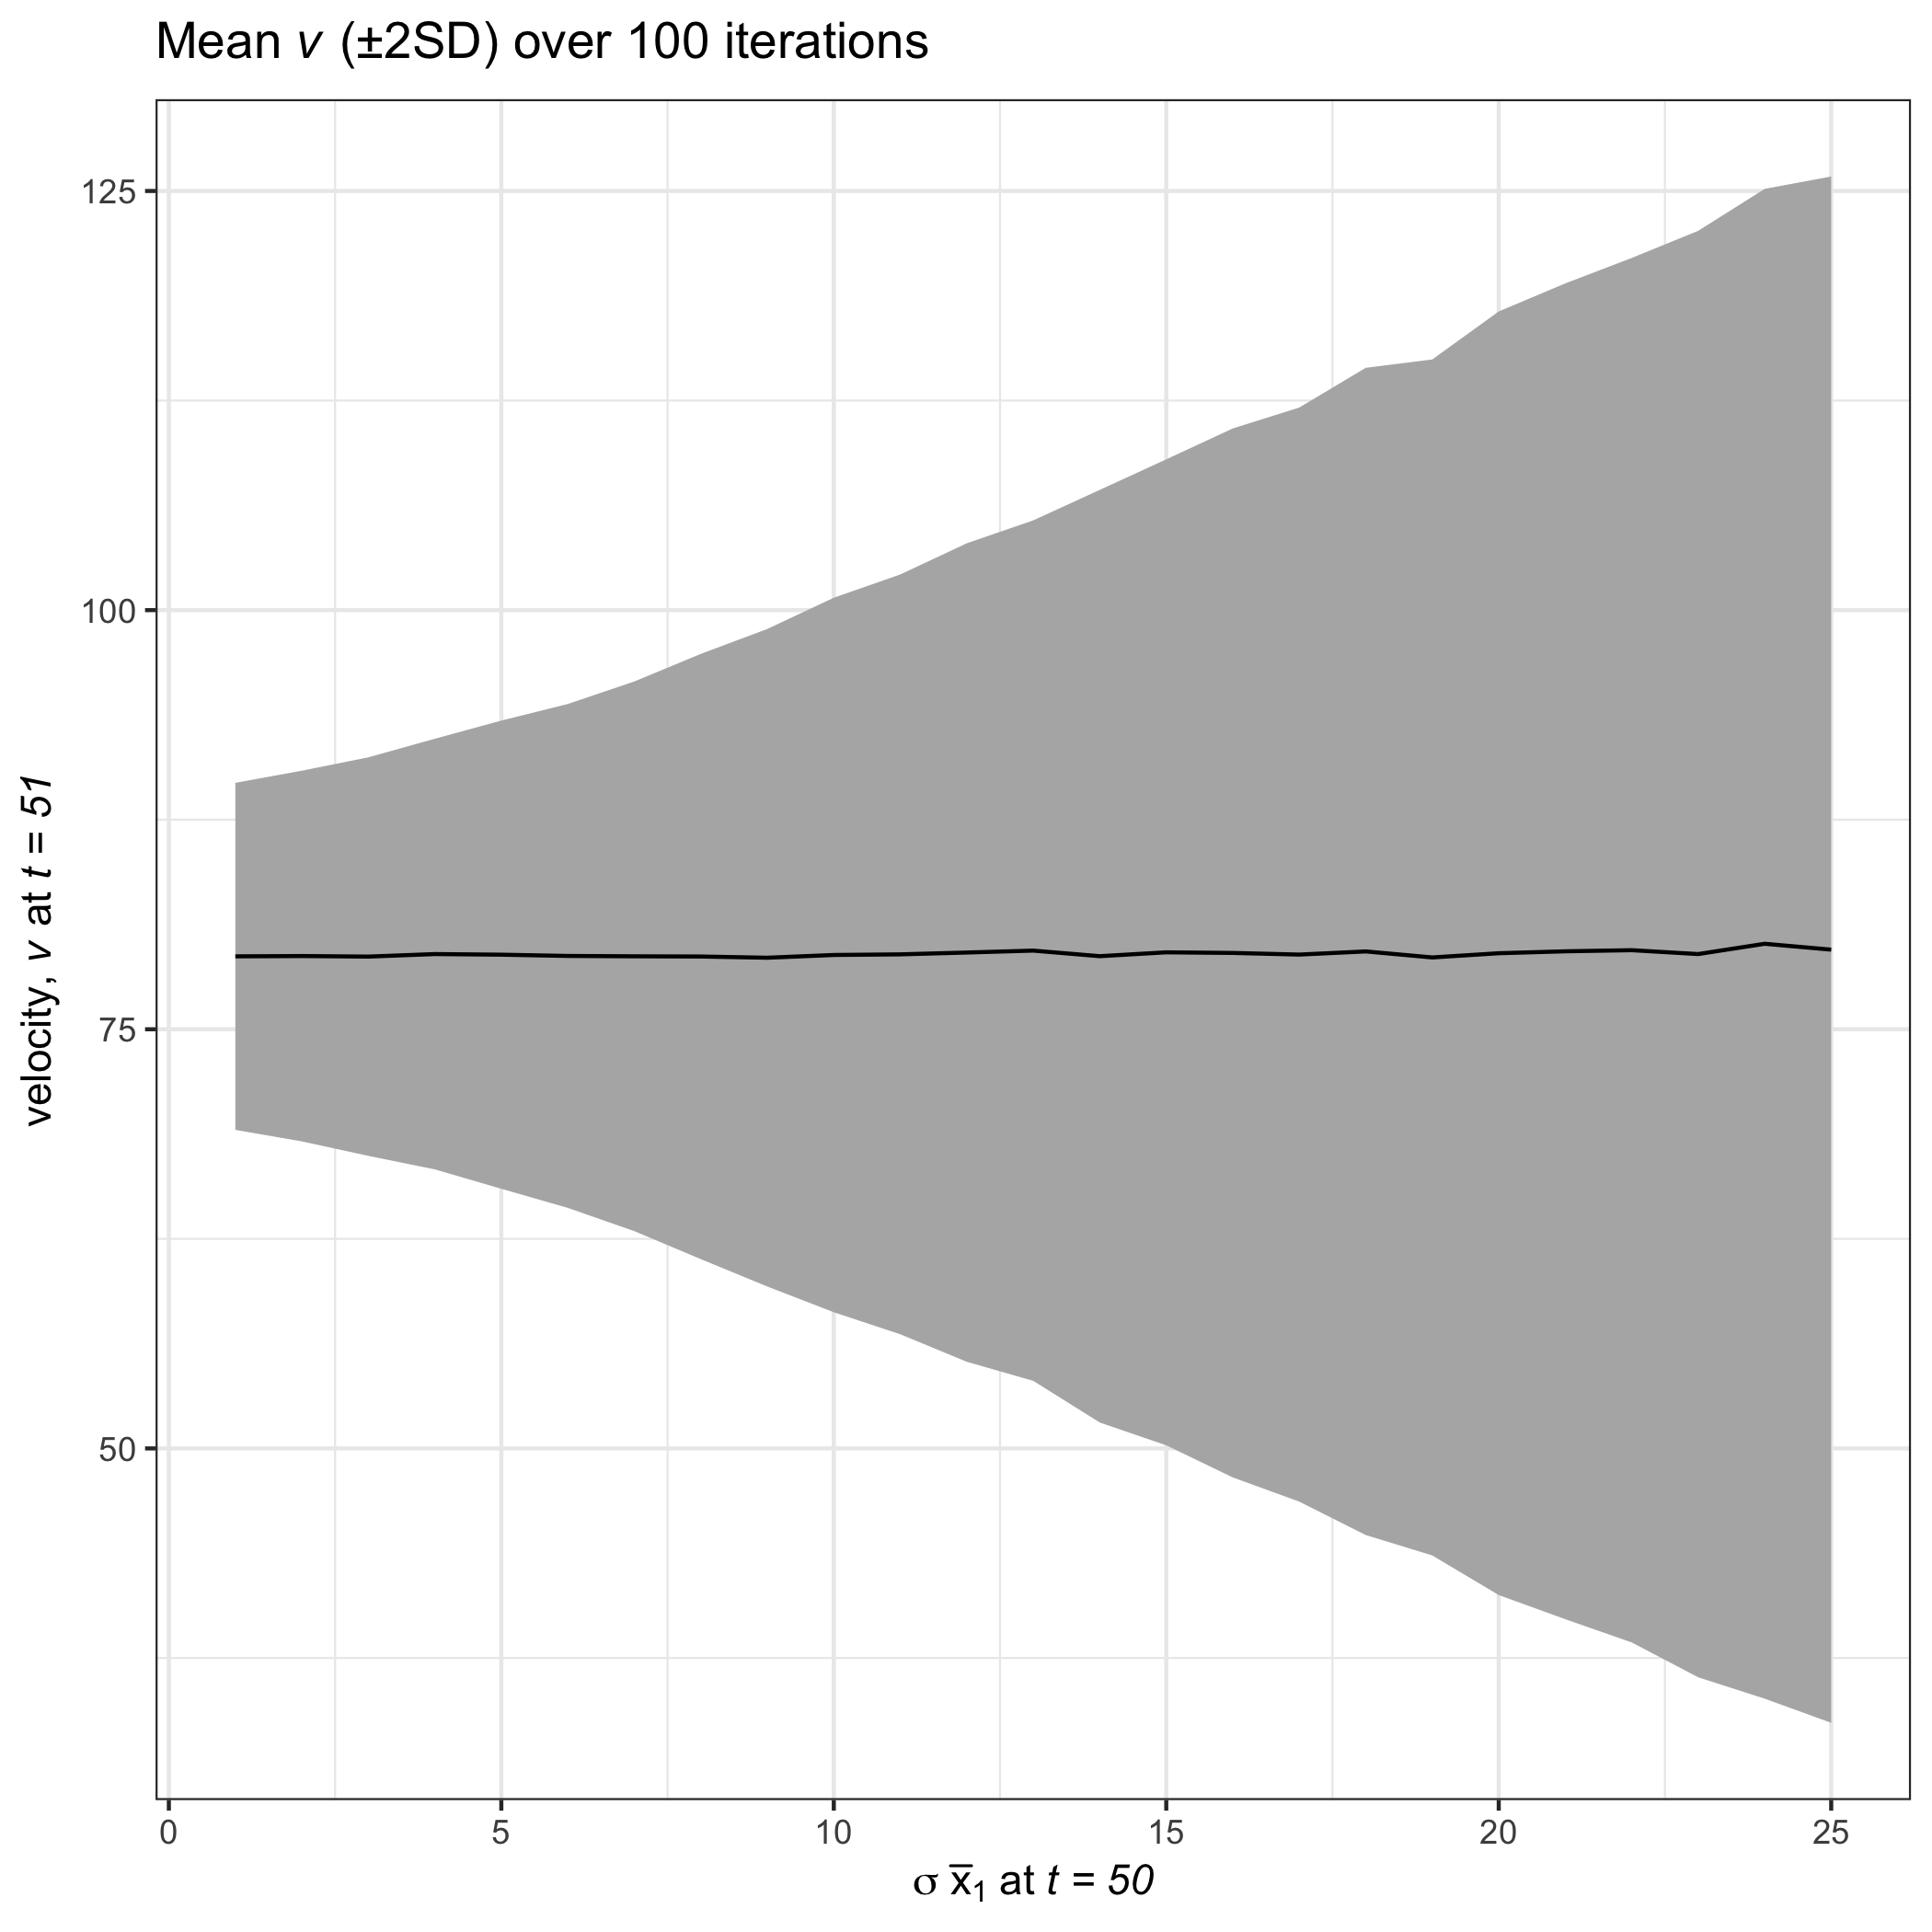
\includegraphics[width=0.65\linewidth]{E:/GitHub/myDissertation/chapterFiles/velocity/figsCalledInDiss/simVarPlot2} 

}

\caption{Average ($\pm 2$ SD) velocity ($v$) worsens as the variance of $\bar{x}_{2_{t=50 (post)}}$ (post shift) increases. $\bar{x}_{1_{pre}} = 25$, $\bar{x}_{1_{post}} = 100$, $\bar{x}_{2_{pre}} = 25$, $\bar{x}_{2_{post}} = 50$, $\sigma_{1_{pre}} = 5$, $\sigma_{2_{pre,post}} = 5$}\label{fig:simVarPlot2}
\end{figure}

Sytem velocity \(v\) appears senstive to increases in the variance at
the point of the regime shift (Figs. @ref(fig:simVarplot),
@ref(fig:simVarplot2)). Again, because velocity is a function of the
total change in the state variables, the variability of \(v\) will
increase with both \(mu\) and \(\sigma\) (Fig. @ref(fig:simVarplot2)).
Further, it is unsurpirsing that \(v\) exhibits sensitivity to changes
in \(\sigma_{post}\) because, without prior smoothing of the data, the
tangential speed of a `noisy' variable will always be noisy itself (see
Figs. @ref(velocitySysEx1), @ref(velocitySysEx2), @ref(velocitySysEx3),
@ref(velocitySysEx4)).

\hypertarget{smoothing-the-data-prior-to-calculating-v}{%
\paragraph{\texorpdfstring{Smoothing the data prior to calculating
\emph{v}}{Smoothing the data prior to calculating v}}\label{smoothing-the-data-prior-to-calculating-v}}

To determine whether process or observational noise influences the
signal in \(v\), I used linear approximation techniques to smooth the
data prior to calculating the derivatives. I used the function
\emph{stats::approx} which linearaly interpolates the original data,
\(x_1\) and \(x_2\), to regularly-spaced time points along the set
\(t=\{1:100\}\). I then calculated \(v\) as described in (Eqs.
@ref(eq:diffX):@ref(eq:velocity)). Increasing the number of points
(\(t\)) at which the original state variables were smoothed (i.e.,
\(t\)) did not influence the amount of noise surrounding the signal of
the regime shift (at \(t=50\)) in system velocity, \(v\) (Fig.
@ref(fig:smoothV)).

\begin{figure}

{\centering 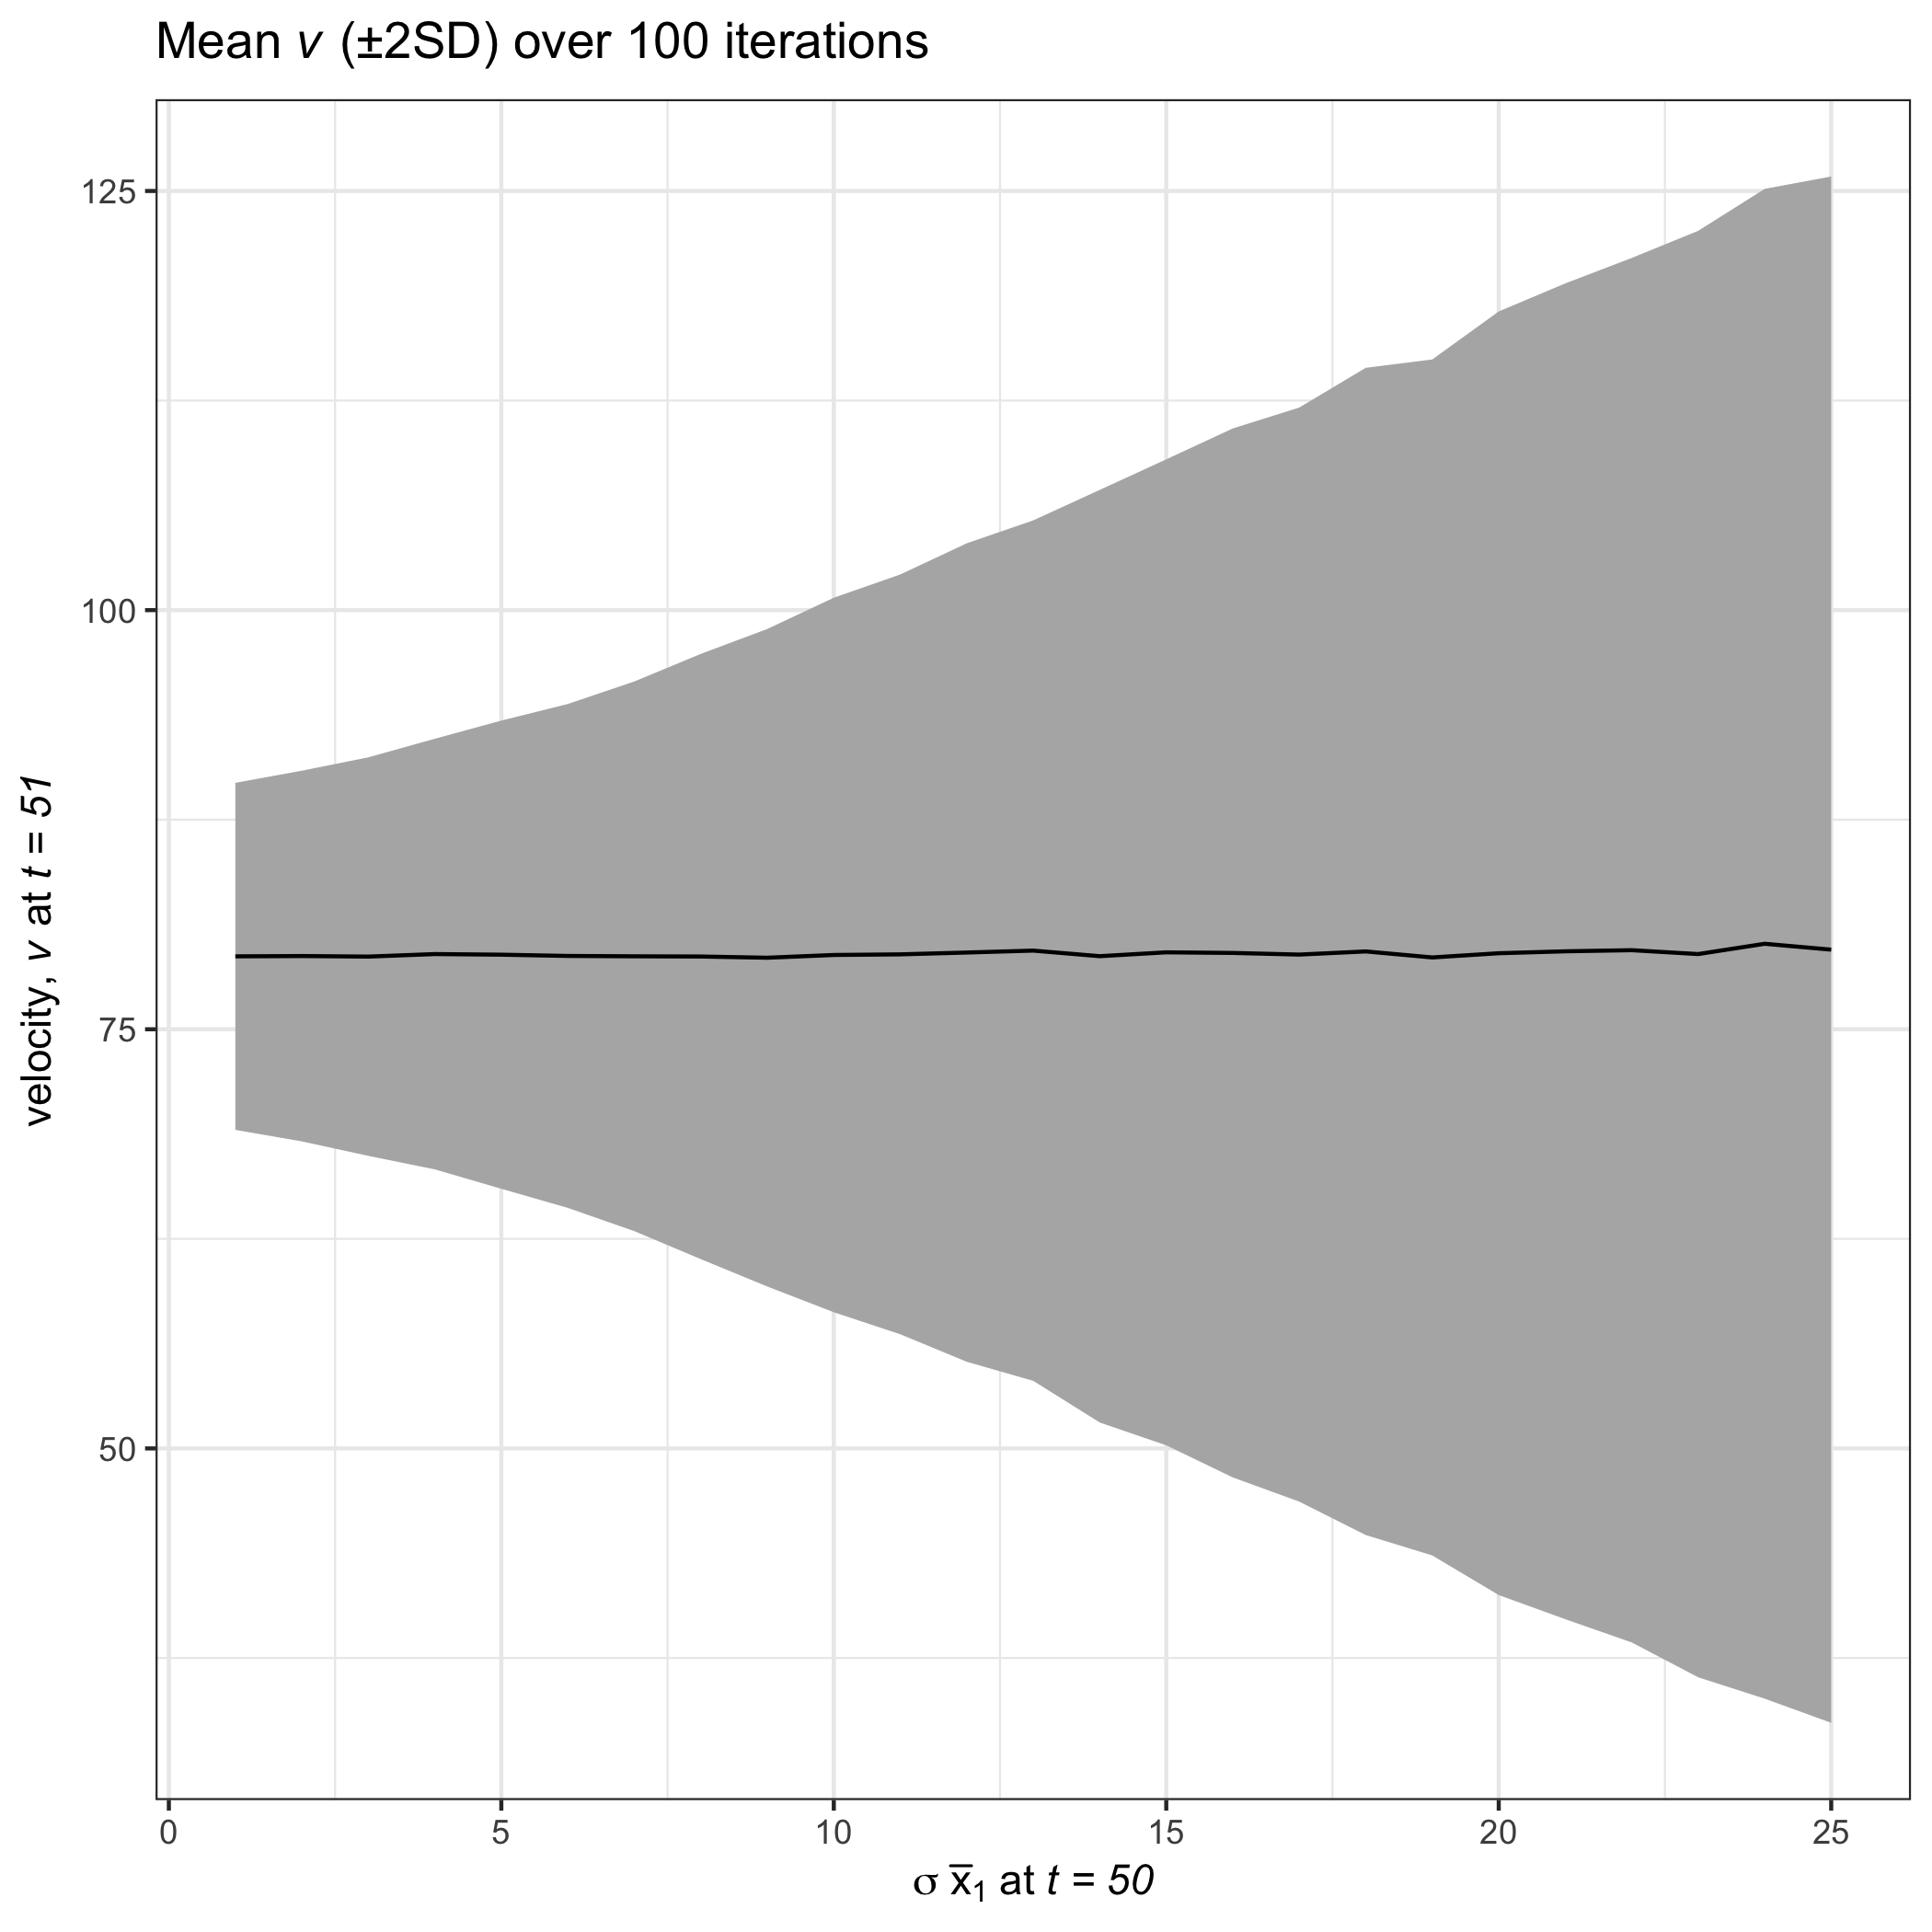
\includegraphics[width=0.55\linewidth]{E:/GitHub/myDissertation/chapterFiles/velocity/figsCalledInDiss/smoothV} 

}

\caption{The noise in system velocity ($v$) is not obviously reduced in this system as the original data ($x_1$, $x_2$) is increasingly smoothed.}\label{fig:smoothV}
\end{figure}

\hypertarget{velocity-performance-under-a-smooth-transition}{%
\subsection{Velocity performance under a smooth
transition}\label{velocity-performance-under-a-smooth-transition}}

In the previous section I presented expectations for velocity signals
under a discontinuous transition in a discrete-time system. Given
velocity is a measure of the rate of a change in a system and the range
of transition speeds ecological systems exhibit (e.g., slow
driver-response or threshold dynamics), it is important to understand if
and when the velocity signal is dampened under varying degrees of
transition speeds. In this section I use a similar toy system, to
demonstrate the expectations of velocity under a smooth shift and under
varying degrees of rapidity.

Although the data constructed in this section are similar to that used
in the previous section in that we are manipulating the mean and
variance of two state variables before and/or after an abrupt shift,
this section introduces a component of process noise into the shift
itself. This is important because the derivative of a nearly
discontinuous function is infinite. Although we are interested in
identifying rapid shifts in systems, velocity will appraoch infinity as
the rate of change in the shift increases and the sampling intervals
decrease. In other words, if the system exhibits turnover in
e.g.~\(25\%\) of the state variables, we expect the value of velocity to
be similar to that of a turnover in e.g.~\(75\%\) of the variables.
Removing the possibility of infinite values provides more relative
measures within the community time series.

\hypertarget{generating-the-data}{%
\subsubsection{Generating the data}\label{generating-the-data}}

Here we consider a two-variable system over the time interval
\([1,100]\) with state variables \(x_1\) and \(x_2\) which exhibits
abrupt shifts in mean and/or variance of one or both variables at time
\(t=50\). I generated species observations for the true process and the
true process with process variability. The true process data were
created using the paramters for \(\mu\) and \(\sigma\) for each of the
conditions in described in Table @ref(tab:sysParams) (random seed in
Program R was 12345).

\begin{table}[t]

\caption{\label{tab:sysParams}Conditions for generating various scenarios of the hyperbolic tangent-induced abrupt change. $\sigma_i$ represents the standard deviation of $\mu_{x_i}$ as the percent of $\mu_{x_i}$, $\mu_{x_i}$ is the mean of the state variable, $x_i$, and pre and post represent the periods before and after the regime shift at $t=50$, respectively.}
\centering
\begin{tabular}{lllllllll}
\toprule
conditions & $\sigma_{x_{1_{pre}}}$ & $\sigma_{x_{1_{post}}}$ & $\sigma_{x_{2_{pre}}}$ & $\sigma_{x_{2_{post}}}$ & $\mu_{x_{1_{pre}}}$ & $\mu_{x_{1_{post}}}$ & $\mu_{x_{2_{pre}}}$ & $\mu_{x_{2_{post}}}$\\
\midrule
$\mu_{x_1}$, $\mu_{x_2}$, $\sigma_{x_1}$, $\sigma_{x_2}$ & 0.05 & 0.10 & 0.05 & 0.10 & 10 & 55 & 15 & 44\\
$\mu_{x_1}$, $\sigma_{x_1}$ & 0.05 & 0.10 & 0.05 & 0.05 & 10 & 55 & 15 & 15\\
$\mu_{x_1}$, $\mu_{x_2}$ & 0.05 & 0.05 & 0.05 & 0.05 & 10 & 55 & 15 & 44\\
$\mu_{x_1}$ & 0.05 & 0.05 & 0.05 & 0.05 & 10 & 55 & 15 & 15\\
$\sigma_{x_1}$, $\sigma_{x_2}$ & 0.05 & 0.10 & 0.05 & 0.10 & 10 & 10 & 15 & 15\\
\addlinespace
$\sigma_{x_1}$ & 0.05 & 0.10 & 0.05 & 0.05 & 10 & 10 & 15 & 15\\
\bottomrule
\end{tabular}
\end{table}

\hypertarget{true-process-model}{%
\paragraph{True process model}\label{true-process-model}}

Data were generated from a normal distribution and an abrupt shift in
the mean was incorporated using a hyperbolic tangent function. The true
process for each state variable, \(x_i\), was generated from Eq.
(@ref(eq:true) (Fig. @ref(fig:trueObsEx))): \begin{equation}
\mu_x{_i{_{pre}}}\sim Normal(\mu_x{_i{_{pre}}},\sigma_x{_i{_{pre}}}) \\ 
\mu_x{_i{_{post}}} \sim Normal(\mu_x{_i{_{pre}}}, \sigma{_i{_{post}}}) \\ 
\mu_{x_i}(t) = \mu_x{_i{_{pre}}}  - 0.5(\mu_x{_i{_{pre}}}-\mu_x{_i{_{post}}})(\tanh(\alpha (t-t_{shift}))+1) \\
(#eq:true)
\end{equation}

where \(\mu_{x_i}(t)\) is the mean value of \(x_i\) at time \(t\) and
\emph{pre} and \emph{post} are the periods before and after the abrupt
shift (\(t_{shift}\)), respectively. The parameter \(\alpha\) in Eq.
@ref(eq:true) controls for the rate of change at the point of the abrupt
change, \(t_{shift}\), where higher values of \(\alpha\) correspond with
a higher slope at \(t_{shift}\). I simulated a single iteration
(dataset) for various conditions of changing \(\mu_x{_i}\) and
\(\sigma_x{_i}\) (see Table @ref(tab:sysParams)), for two state
variables \(x_1\ \&\ x_2\) at intervals of \(t=1\) along the temporal
interval \(t=[1,100]\). \textbackslash{}begin\{figure\}

\{\centering 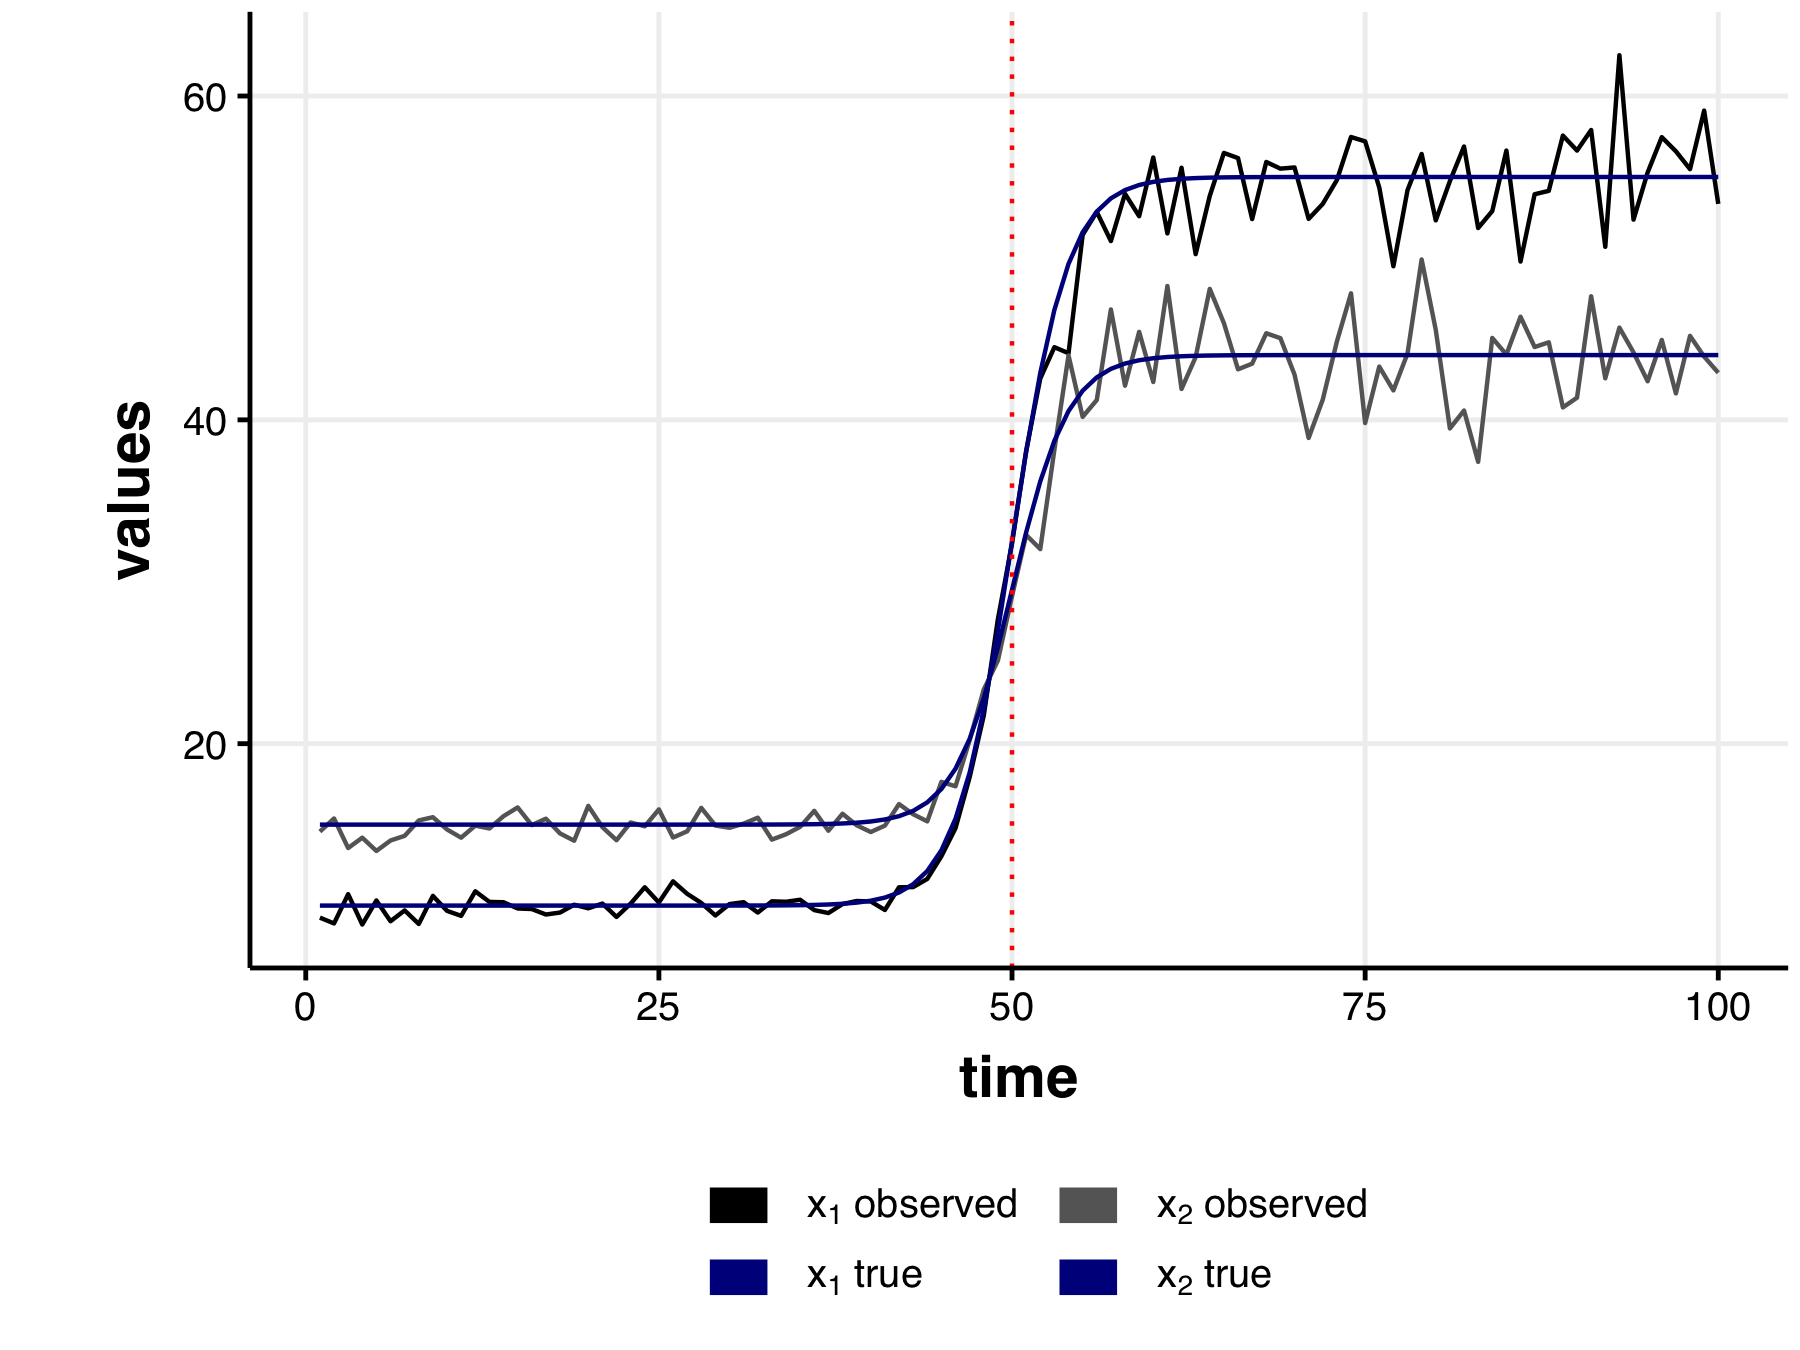
\includegraphics[width=0.65\linewidth]{E:/GitHub/myDissertation/chapterFiles/velocity/figsCalledInDiss/changeMuBoth_tanhAlpha0.25-0.5tvdiffAlpha-1000iter_origDat}

\}

\textbackslash{}caption\{An example of the data generated by the true
process model. In this example the mean values (\(\mu{_x{_i}}}\)), but
not the percent standard deviation (\(\sigma_x{_i}}\)), are varied
before and after the transition point. The observed data are plotted
against the true-process model for each state variable, \(x_i\). Panels
represent different degrees of the smoothing parameter, \(\alpha\) (top:
\(\alpha=0.25\), bottom:\(\alpha=1.00\)).\}\label{fig:trueObsEx}
\textbackslash{}end\{figure\} \textbackslash{}begin\{figure\}

\{\centering 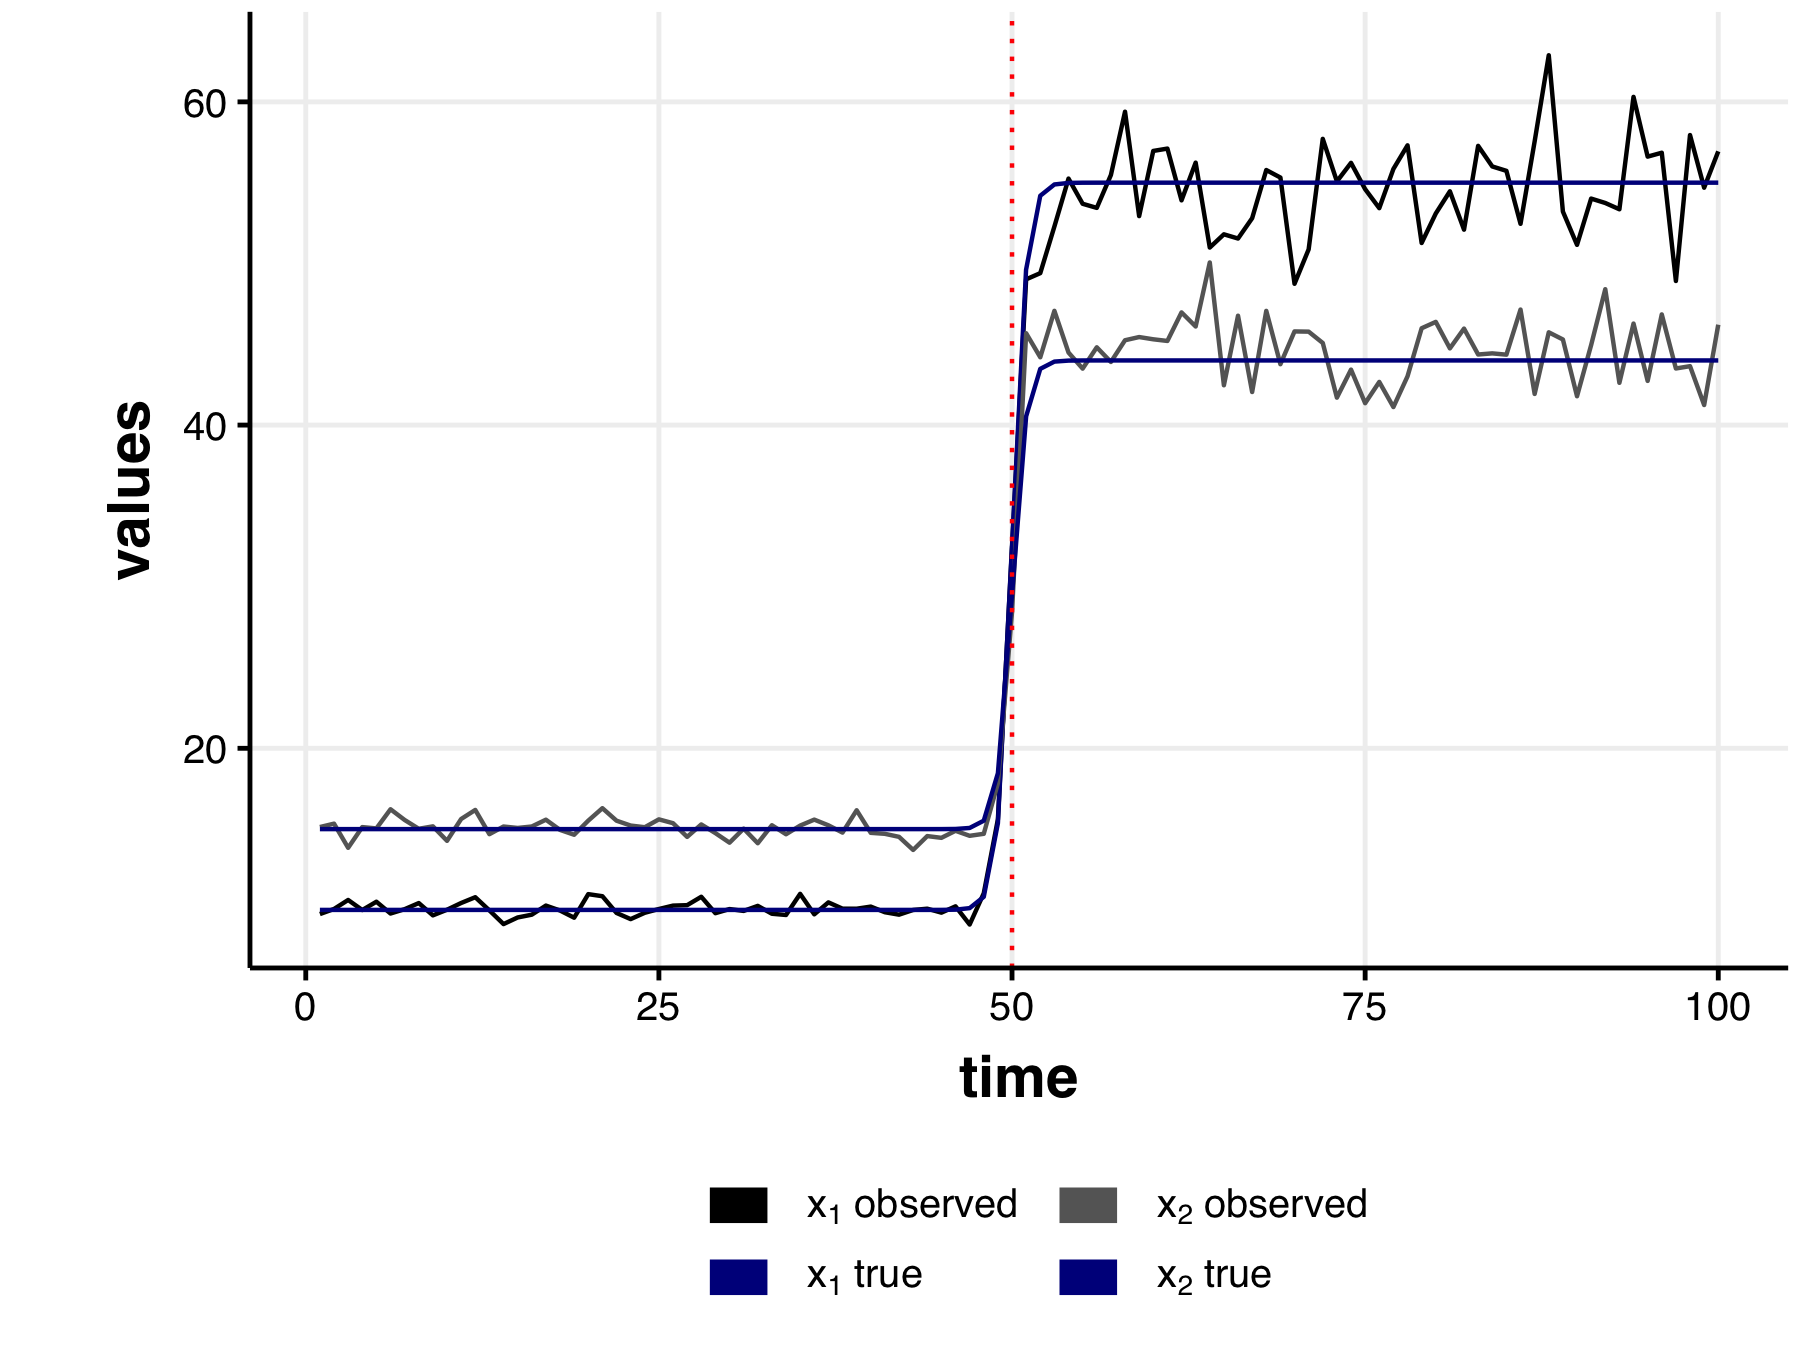
\includegraphics[width=0.65\linewidth]{E:/GitHub/myDissertation/chapterFiles/velocity/figsCalledInDiss/changeMuBoth_tanhAlpha1-100tvdiffAlpha-1000iter_origDat}

\}

\textbackslash{}caption\{An example of the data generated by the true
process model. In this example the mean values (\(\mu{_x{_i}}}\)), but
not the percent standard deviation (\(\sigma_x{_i}}\)), are varied
before and after the transition point. The observed data are plotted
against the true-process model for each state variable, \(x_i\). Panels
represent different degrees of the smoothing parameter, \(\alpha\) (top:
\(\alpha=0.25\), bottom:\(\alpha=1.00\)).\}\label{fig:trueObsEx}
\textbackslash{}end\{figure\}

\hypertarget{observed-process-data}{%
\paragraph{Observed process data}\label{observed-process-data}}

I generated observations by imputing noise into the true process model
(Eq. @ref(eq:true)) through random sampling of \(\sigma_x{_i}\) from a
normal distribution (Eq. @ref(eq:observed); Fig. @ref(fig:trueObsEx)):
\begin{equation}
\mu_x{_i{_{pre}}}\sim Normal(\mu_x{_i{_{pre}}},\sigma_x{_i{_{pre}}}) \\ 
\sigma_x{_i{_{pre}}} \sim Normal(0,\sigma_X{_i{_{pre}}}\mu_x{_i{_{pre}}}) \\
\mu_x{_i{_{post}}} \sim Normal(\mu_i_{post},\sigma_i_{post}) \\ 
\sigma_x{_i{_{post}}} \sim Normal(0,\sigma_X{_i{_{post}}}\mu_x{_i{_{post}}}) \\
\mu_{x_i}(t) = \mu_x{_i{_{pre}}}  - 0.5(\mu_x{_i{_{pre}}}-\mu_x{_i{_{post}}})(\tanh(\alpha (t-t_{shift}))+1) \\
(#eq:observed)
\end{equation}

where \(\sigma_x_i\) is the observed error around \(\mu_x_i\), and
\(\sigma_X_i\) is \(X\%\) of \(\mu_x_i\) under various sampling
conditions (as described in Table @ref(tab:sysParams)). I generated the
error as a percent of the mean as this scaling relationship is commonly
observed in ecological data {[}@taylor1961aggregation{]}.

\hypertarget{evaluating-velocity-performance-under-conditions-of-changing-means-andor-variance}{%
\subsubsection{Evaluating velocity performance under conditions of
changing means and/or
variance}\label{evaluating-velocity-performance-under-conditions-of-changing-means-andor-variance}}

I simulated a single dataset (R seed 12345) by randomly drawing a single
realisation (observed data) of the hyperbolic tangent process model with
additive process noise (Eq. @ref(eq:observed)). I then calculated the
distance travelled, \(s\), and the velocity of the distance travelled,
\(v\) (also referred to as \(\frac{ds}{dt}\)) using first differences.
The first differences approach is a simple alternative to numerical
integration tecniques, requiring only simple algebraic techniques. This
method is ideal for discrete time data, or where computational power
woudl not suffice for numerical integration. When using the first
differences method, however, \(v\) will demonstrate high variability,
depending on the amount of time between samples (i.e.~as the intervals
of \(t-t+1\) increase).

I also calculated \(v\) using a numerical integration method for
non-smooth, noisy data, called total variation regularized
differentiation {[}@chartrand2011numerical{]}. I used the R package
\texttt{tvdiff} {[}@price2019tvdiff{]} to perform numerically integrate
the distance travelled, \(s\). The regularized differentiation method in
this package {[}function `tvRegDiff`; descried fully in
@chartrand2011numerical{]} provides a numerical solution for calculating
non-noisy derivatives of noisy, non-smooth data. Using this
smooth-derivative estimation technique may be an ideal supplement to the
velocity method in cases where process and observational error generate
noisy observational data. Although not possible in most ecological
systems data, here we can compare the fit of the smooth-derivative to
the derivative of the true process, allowing us to determine the
usefulness of calculating a smooth-derivative. There are two tuning
paramters required to be chosen by the analyst when implementing the
total-variation regularized differentiation, each of which influence the
amount of noise smoothed out in the resulting derivative: \(\alpha\) and
the number of iterations. I implemented this numerical differentiation
over 1,000 iterations, and selected \(\alpha\) by comparing the
antidifferentiated distance travelled, \(s\), to the true process values
of \(s\) (e.g., see Figure @ref(fig:antiDiffComp)). For most conditions
and smoothness I found the tuning parameter for \texttt{tvdiff}
\(\alpha=0.50\) provided a good fit of \(s\) (Fig.
@ref(fig:antiDiffComp)), however, when the hyperbolic tangent smoothing
paramter, \(\alpha\) was low (i.e.~\(\alpha_{tanh}=0.25\)) higher values
of \(\alpha_{tvdiff}\) yielded more abrupt changes in the derivative.

\hypertarget{smooth-changes-in-the-mean}{%
\paragraph{Smooth changes in the
mean}\label{smooth-changes-in-the-mean}}

As discussed earlier, the velocity of the distance travelled, \(v\), is
a measure of how quickly the sum of the squared system variables change
between observations (i.e.~time). Consequently, as the total change in
state variables grows, so will the maximum potential of the velocity,
\(v\). Following this logic, we should expect to see a spike in the
derivative of the distance travelled when the system changes quickly. I
tested this hypothesis under two conditions of changing means, where
either one or both variables underwent mean shifts (see Table
@ref(tab:params)), and under varying degrees of transition smooothness
(i.e.~\(\alpha_{tanh}={0.25, 0.50, 0.75, 1.00}\)).

When the hyperbolic tangent smooth transition function is less steep
(@ref(fig:mu1var.25)) the observed velocity signal is dampened. This
signal, however, is quickly recovered when the transition function
becomes more abrupt (Figs.
@ref(fig:mu1var.5),@ref(fig:mu1var.75,@ref(fig:mu1var1);
\(\alpha_{tanh}=0.5, 0.75, and 1.00\), respectively). Unsurprisingly,
when we shift the means of both state variables while holding the
relative variance constant, the velocity signal changes more abruptly
(Fig. @ref(fig:muBoth.25)) than when only a single variable shifts mean
value (compare with Fig. @ref(mu1Var.25)). Figure @ref(muBoth.75) is
representative of the increasing signal in velocity as \(\alpha_{tanh}\)
increases.

\begin{figure}

{\centering 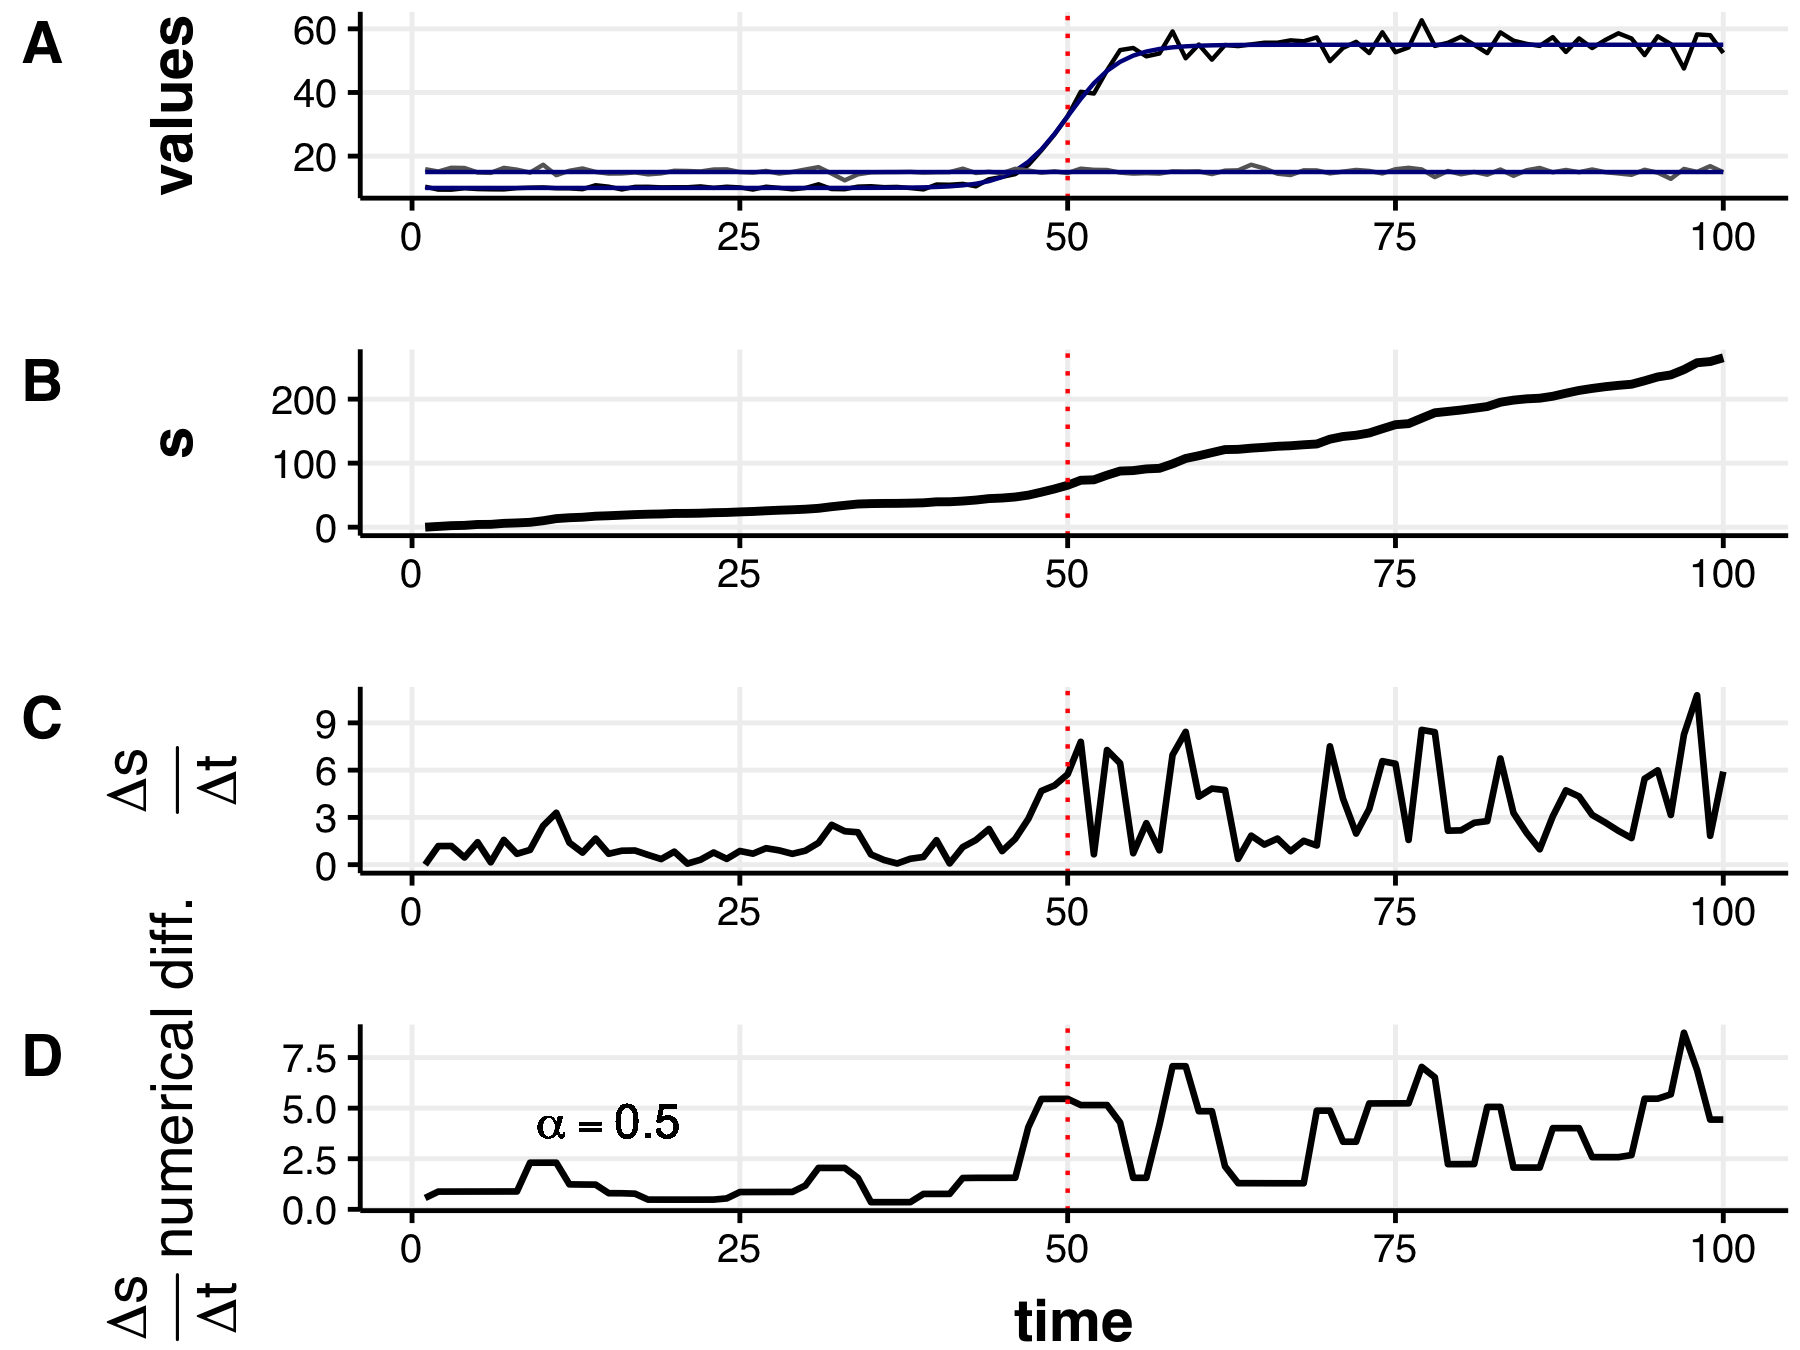
\includegraphics[width=0.65\linewidth]{E:/GitHub/myDissertation/chapterFiles/velocity/figsCalledInDiss/changeMuX1_tanhAlpha0.25-0.5tvdiffAlpha-1000iter_stackTvdiff} 

}

\caption{The velocity signal is muted when the  hyperbolic smoothing parameter, $lpha$, is low (0.25). True and observed values of $x_i$ (panel A), observed distance travelled ($s$, panel B), observed velocity (C), and the smoothed velocity (D). }\label{fig:mu1var.25}
\end{figure}
\begin{figure}

{\centering 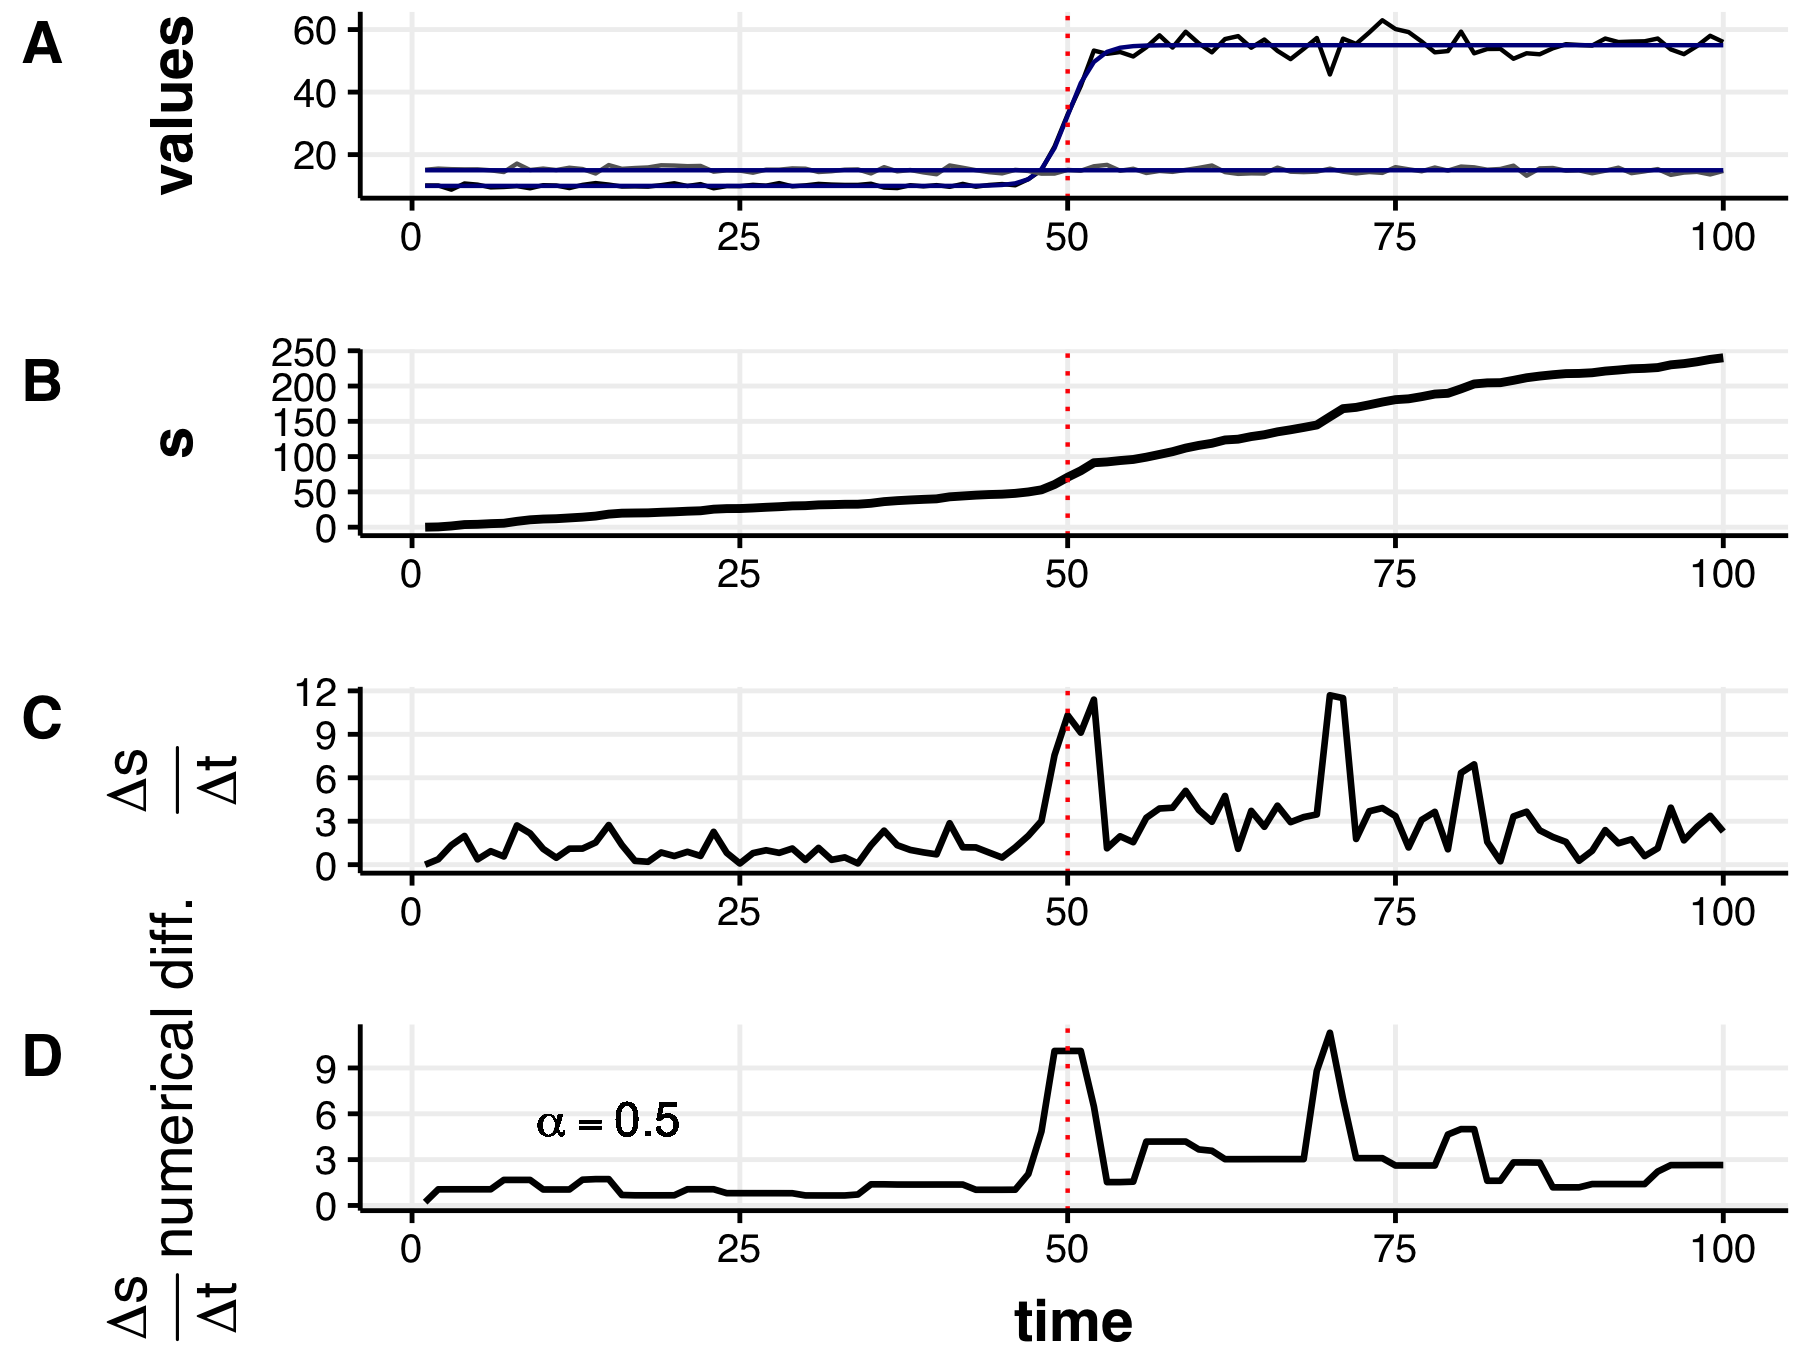
\includegraphics[width=0.65\linewidth]{E:/GitHub/myDissertation/chapterFiles/velocity/figsCalledInDiss/changeMuX1_tanhAlpha0.5-0.5tvdiffAlpha-1000iter_stackTvdiff} 

}

\caption{The velocity signal is muted when the  hyperbolic smoothing parameter, $lpha$, is moderate (0.50). True and observed values of $x_i$ (panel A), observed distance travelled ($s$, panel B), observed velocity (C), and the smoothed velocity (D). }\label{fig:mu1var.5}
\end{figure}
\begin{figure}

{\centering 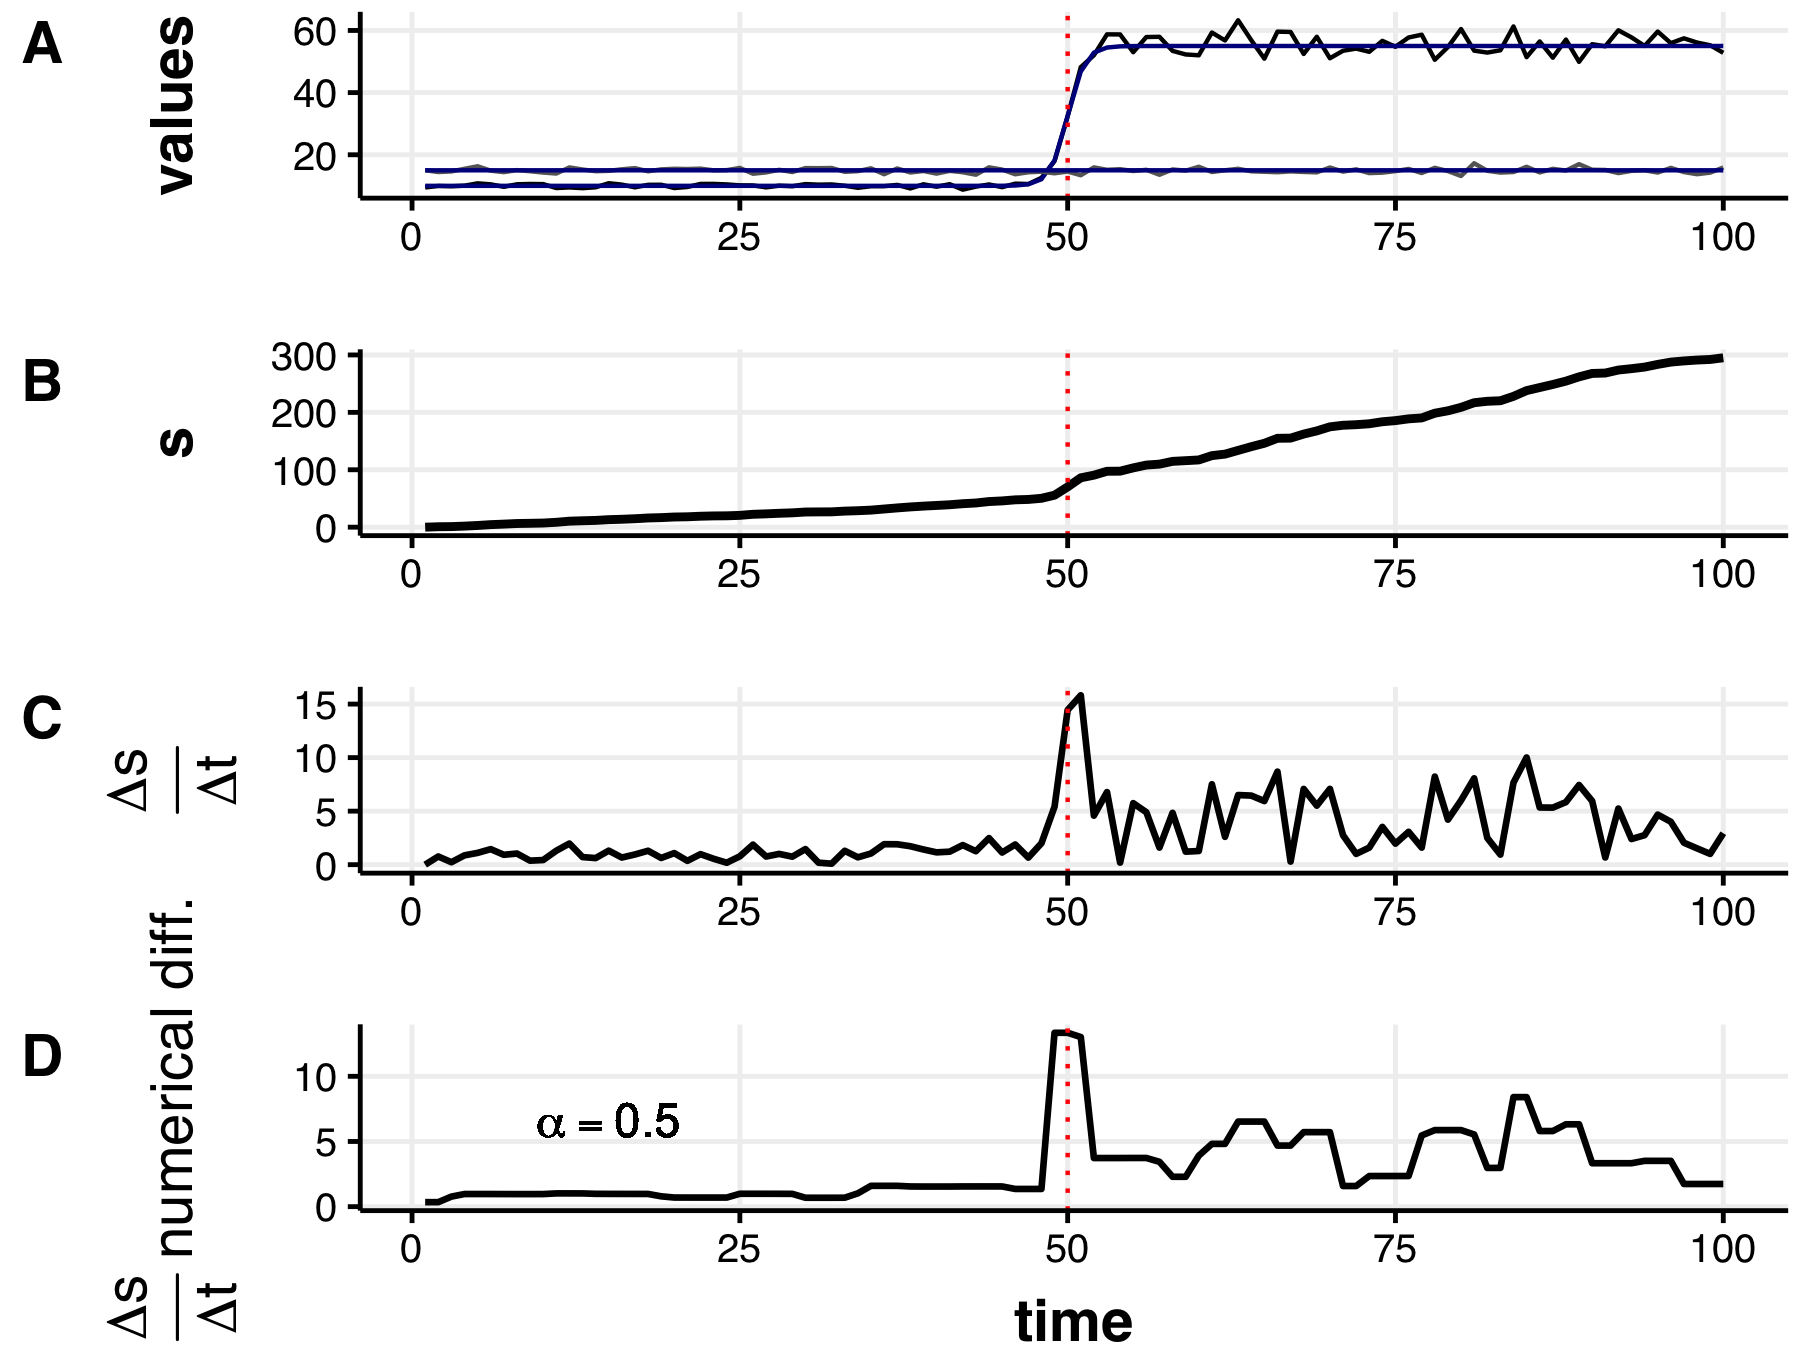
\includegraphics[width=0.65\linewidth]{E:/GitHub/myDissertation/chapterFiles/velocity/figsCalledInDiss/changeMuX1_tanhAlpha0.75-0.5tvdiffAlpha-1000iter_stackTvdiff} 

}

\caption{The velocity signal is muted when the  hyperbolic smoothing parameter, $lpha$, is moderate (0.50). True and observed values of $x_i$ (panel A), observed distance travelled ($s$, panel B), observed velocity (C), and the smoothed velocity (D). }\label{fig:mu1var.75}
\end{figure}
\begin{figure}

{\centering 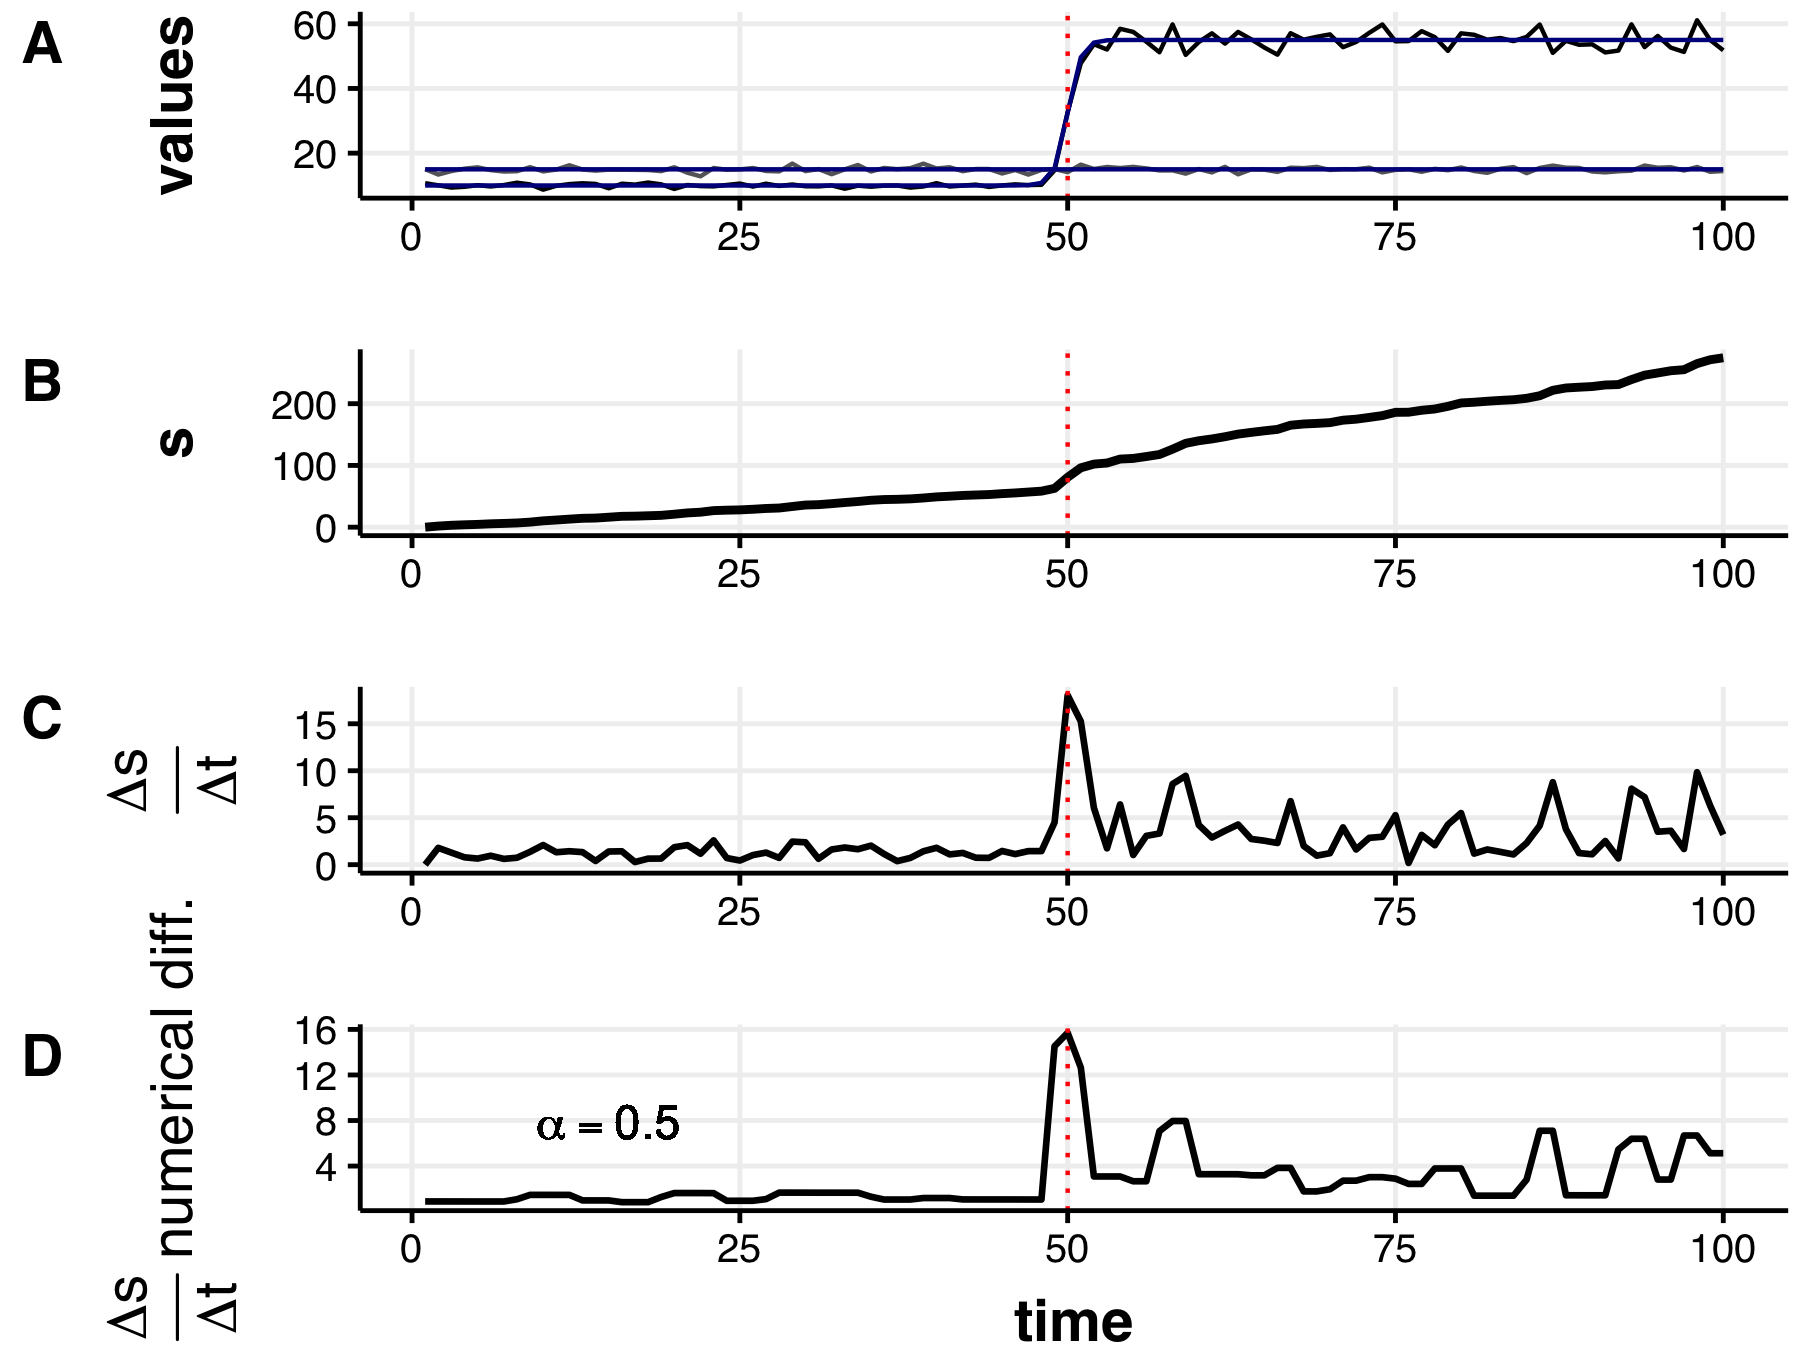
\includegraphics[width=0.65\linewidth]{E:/GitHub/myDissertation/chapterFiles/velocity/figsCalledInDiss/changeMuX1_tanhAlpha1-0.5tvdiffAlpha-1000iter_stackTvdiff} 

}

\caption{The velocity signal is muted when the  hyperbolic smoothing parameter, $lpha$, is moderate (0.50). True and observed values of $x_i$ (panel A), observed distance travelled ($s$, panel B), observed velocity (C), and the smoothed velocity (D). }\label{fig:mu1var1}
\end{figure}
\begin{figure}

{\centering 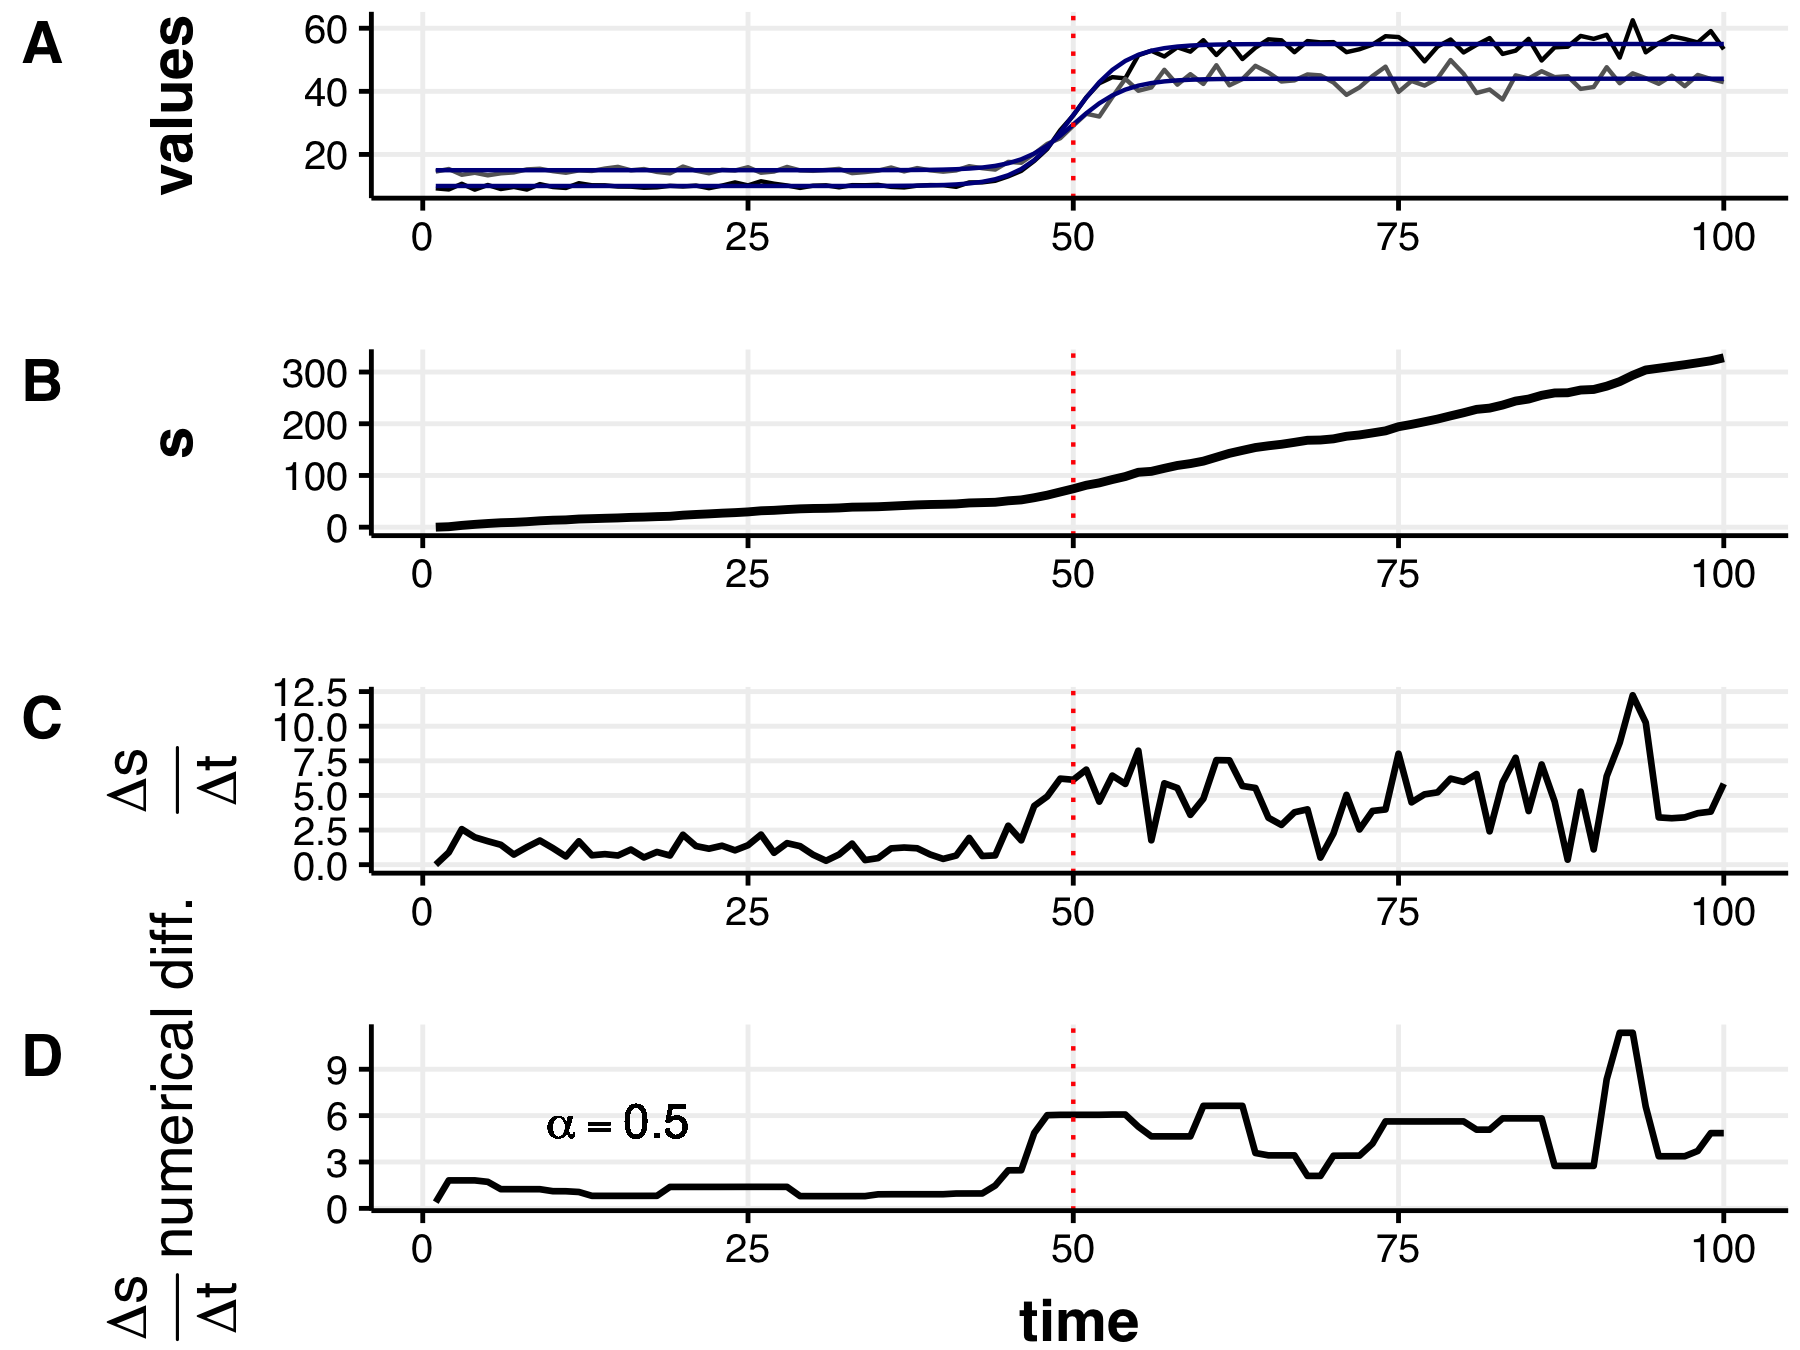
\includegraphics[width=0.65\linewidth]{E:/GitHub/myDissertation/chapterFiles/velocity/figsCalledInDiss/changeMuBoth_tanhAlpha0.25-0.5tvdiffAlpha-1000iter_stackTvdiff} 

}

\caption{The velocity signal is regained under smoooth transition ($lpha_{tanh}=0.25$) when both state variables undergo a shift in the mean. True and observed values of $x_i$ (panel A), observed distance travelled ($s$, panel B), observed velocity (C), and the smoothed velocity (D). }\label{fig:muBoth.25}
\end{figure}
\begin{figure}

{\centering 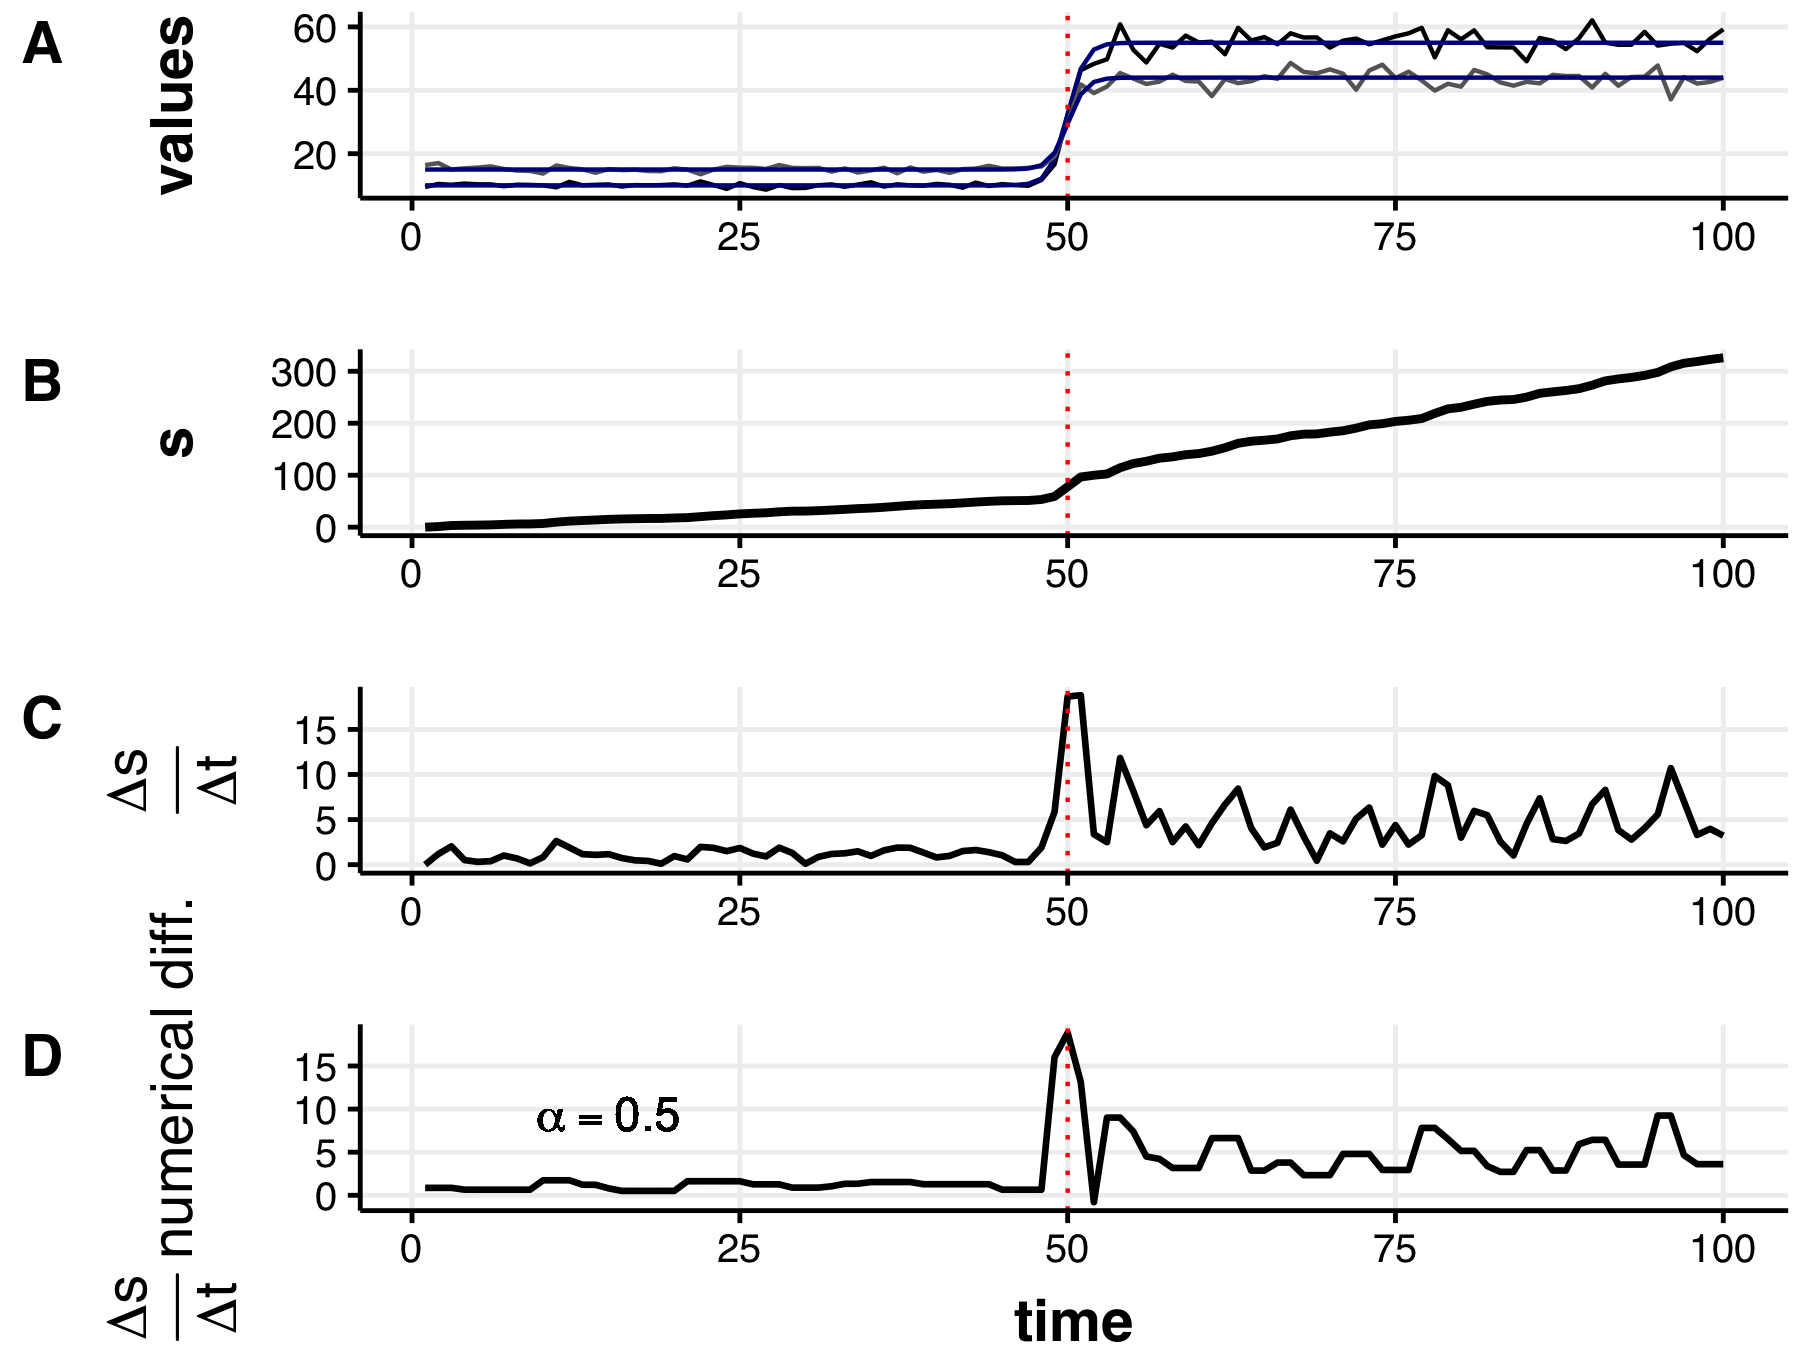
\includegraphics[width=0.65\linewidth]{E:/GitHub/myDissertation/chapterFiles/velocity/figsCalledInDiss/changeMuBoth_tanhAlpha0.75-0.5tvdiffAlpha-1000iter_stackTvdiff} 

}

\caption{The velocity signal is regained under smoooth transition ($lpha_{tanh}=0.75$) when both state variables undergo a shift in the mean. True and observed values of $x_i$ (panel A), observed distance travelled ($s$, panel B), observed velocity (C), and the smoothed velocity (D). }\label{fig:muBoth.75}
\end{figure}

\hypertarget{smooth-changes-in-variance}{%
\paragraph{Smooth changes in
variance}\label{smooth-changes-in-variance}}

Abrupt changes sometimes manifest first as a change in the variability,
rather than the mean value, of the state variables. This condition
manifests in the velocity signal when both variables experience a shift
in relative variance (Fig. @ref(fig:varBoth)), however, does not signal
change when only one variable exhibits a shift in variance (Fig.
@ref(fig:var1)). Again, given the total magnitude of change influences
the distance travelled, \(s\), and the derivative of s, \(v\), it is not
surprising that the velocity signal is greater around the transition
point when both, compared to a single, state variable exhibits increased
variability about the mean. In these scenarios I shifted the variability
in the state variables \(x_i\) from only \(\sim 5\%\) to \(\sim10\%\)
(see Table @ref(tab:params))---this percent variability is low relative
to most empirical observational ecological datasets. As such, I expect
the velocity signal to be more pronounced when empirical systems undergo
shifts in variance in at least one state variable.

\begin{figure}

{\centering 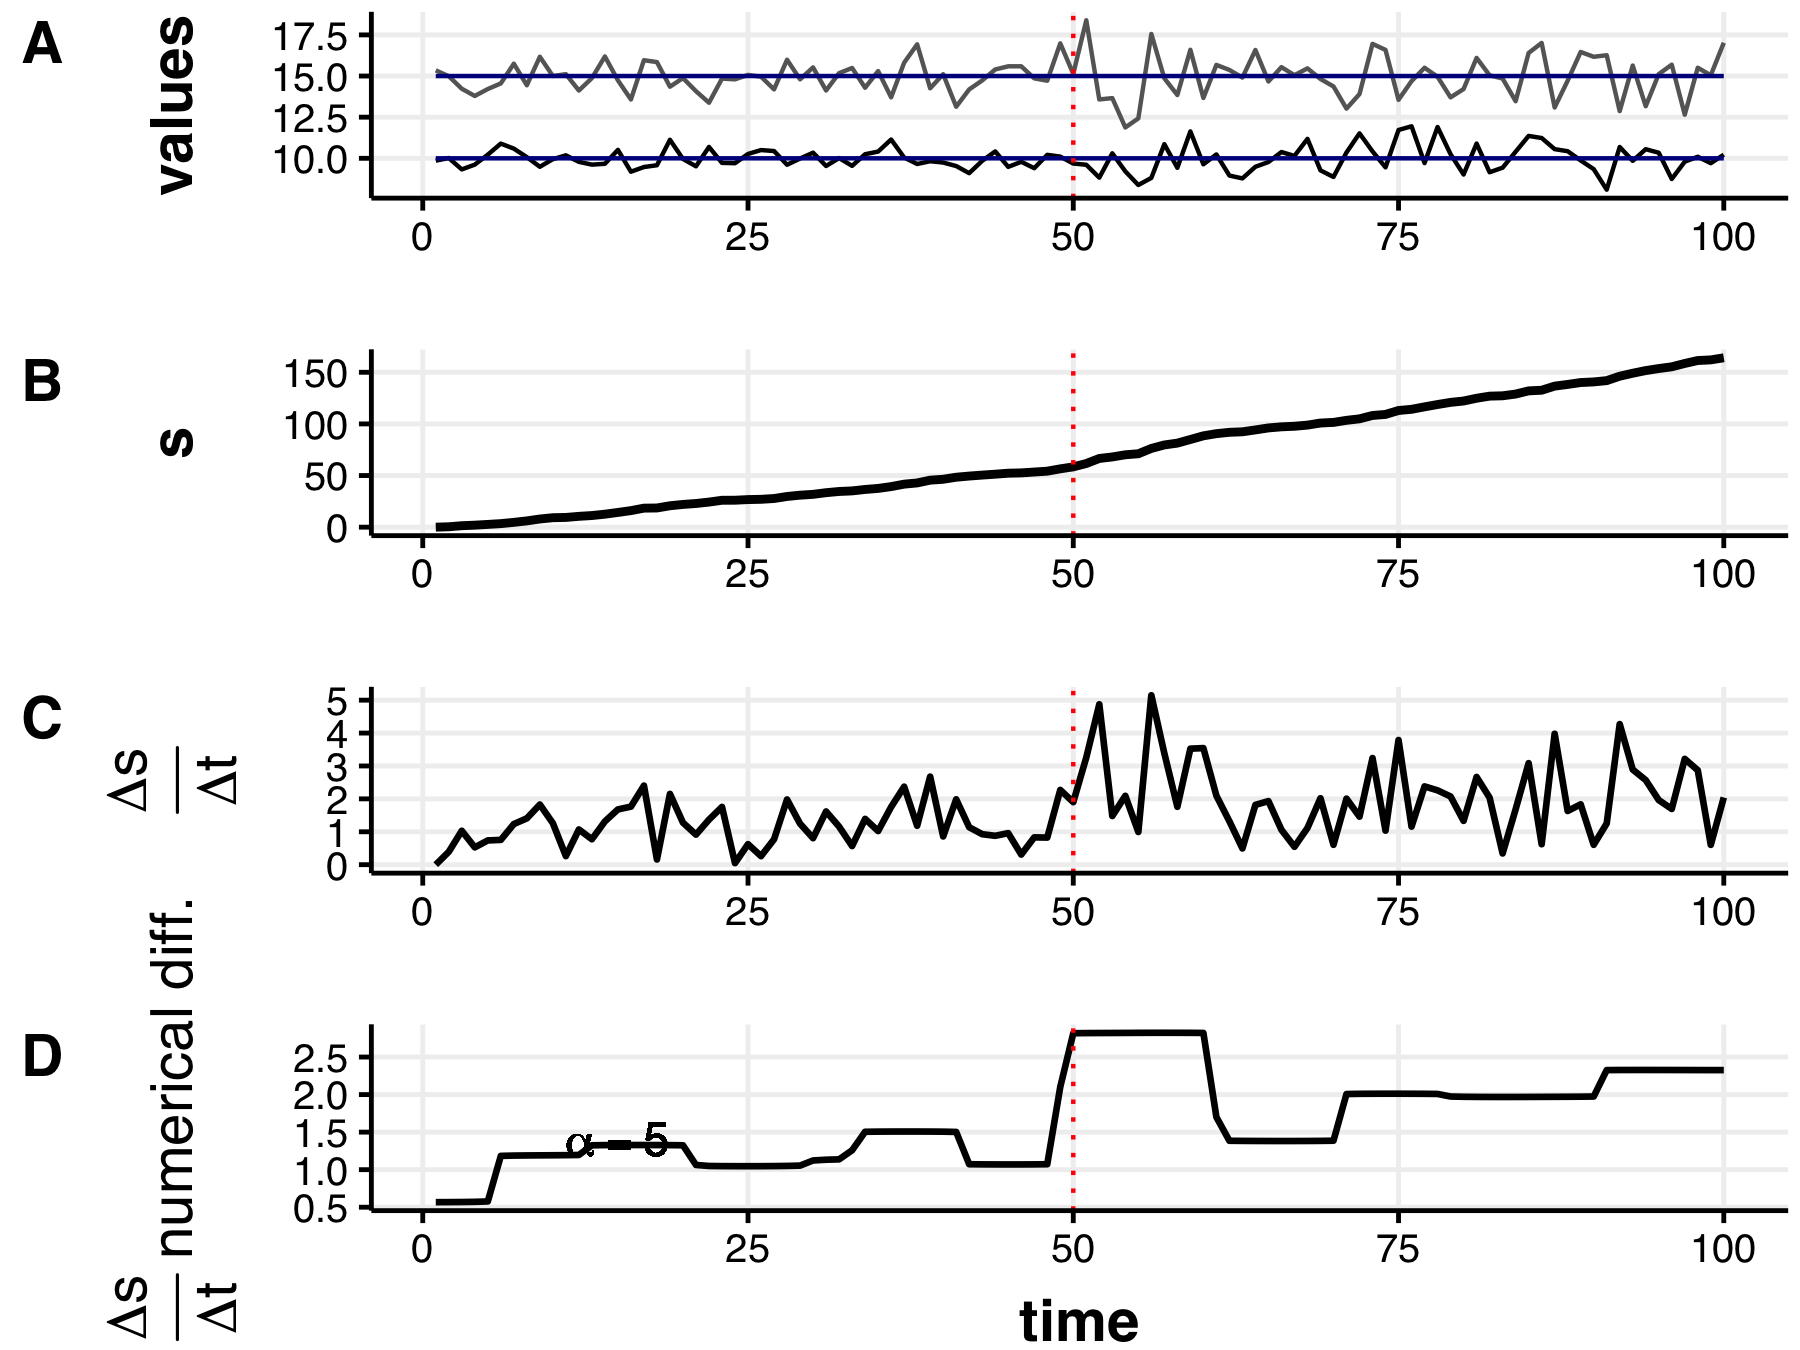
\includegraphics[width=0.65\linewidth]{E:/GitHub/myDissertation/chapterFiles/velocity/figsCalledInDiss/changeVarBoth_tanhAlpha0.75-5tvdiffAlpha-1000iter_stackTvdiff} 

}

\caption{The velocity signals a rapid shift in the variance of both state variables under a moderately abrupt transition ($lpha_{tanh}=0.75$). True and observed values of $x_i$ (panel A), observed distance travelled ($s$, panel B), observed velocity (C), and the smoothed velocity (D). }\label{fig:varBoth}
\end{figure}
\begin{figure}

{\centering 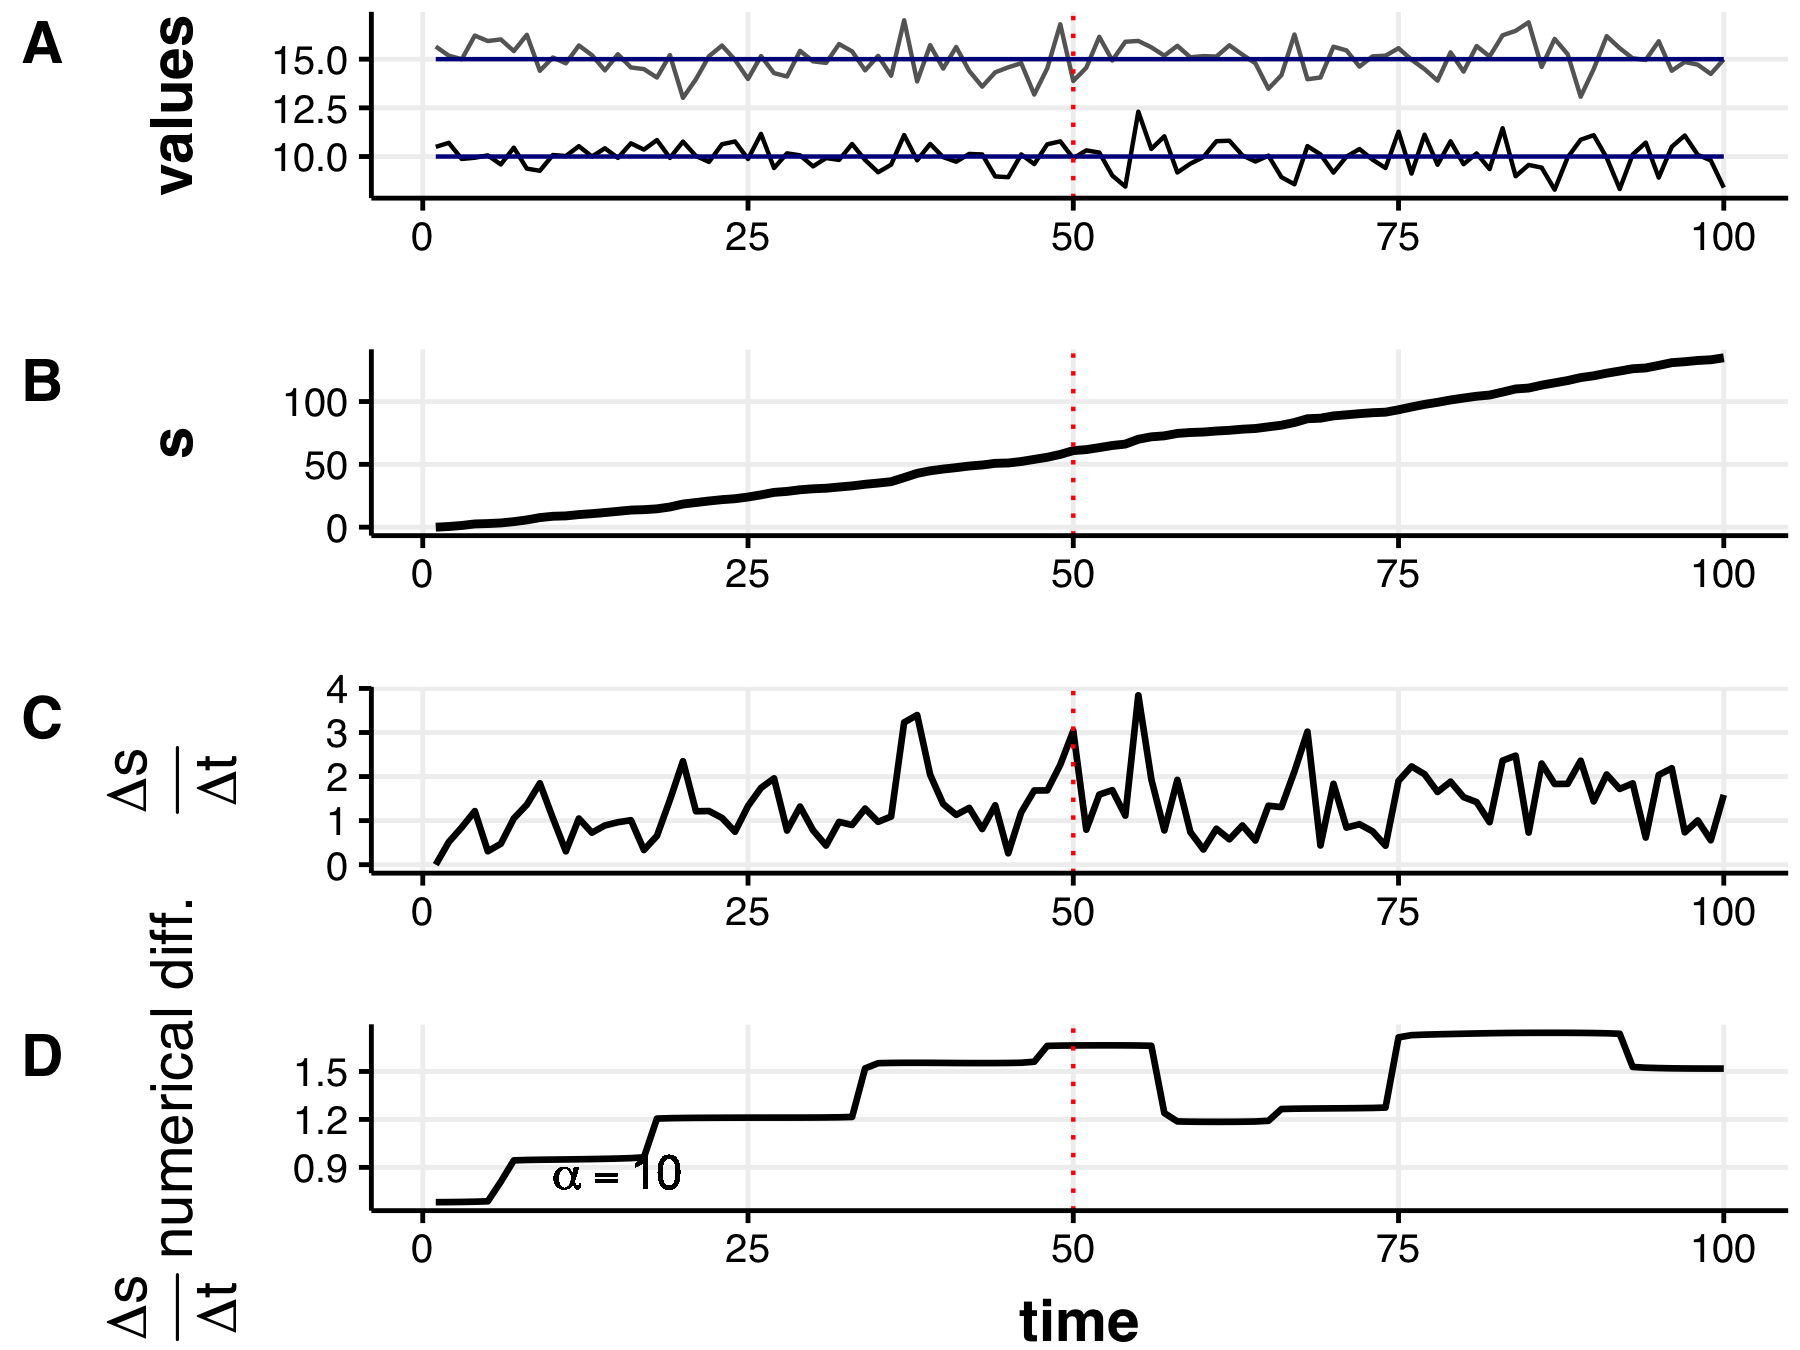
\includegraphics[width=0.65\linewidth]{E:/GitHub/myDissertation/chapterFiles/velocity/figsCalledInDiss/changeVarX1_tanhAlpha0.75-10tvdiffAlpha-1000iter_stackTvdiff} 

}

\caption{The velocity does not signal shifts in the variance of a single variable ($x_1$) under a moderately abrupt transition ($lpha_{tanh}=0.75$). True and observed values of $x_i$ (panel A), observed distance travelled ($s$, panel B), observed velocity (C), and the smoothed velocity (D). }\label{fig:var1}
\end{figure}

\hypertarget{smooth-changes-in-the-mean-and-variance}{%
\paragraph{Smooth changes in the mean and
variance}\label{smooth-changes-in-the-mean-and-variance}}

Given the signals identified in the velocity when one or both state
varialbes exhibits a shift in mean and/or variance, it is unsurprising
that even under smooth transitions (when \(\alpha_{tanh} = 0.25\)),
velocity manifests as a signal of change (Fig. @ref(muVarBoth.25)). This
signal is most pronounced when the shift is abrupt (Fig.
@ref(muVarBoth1))

\begin{figure}

{\centering 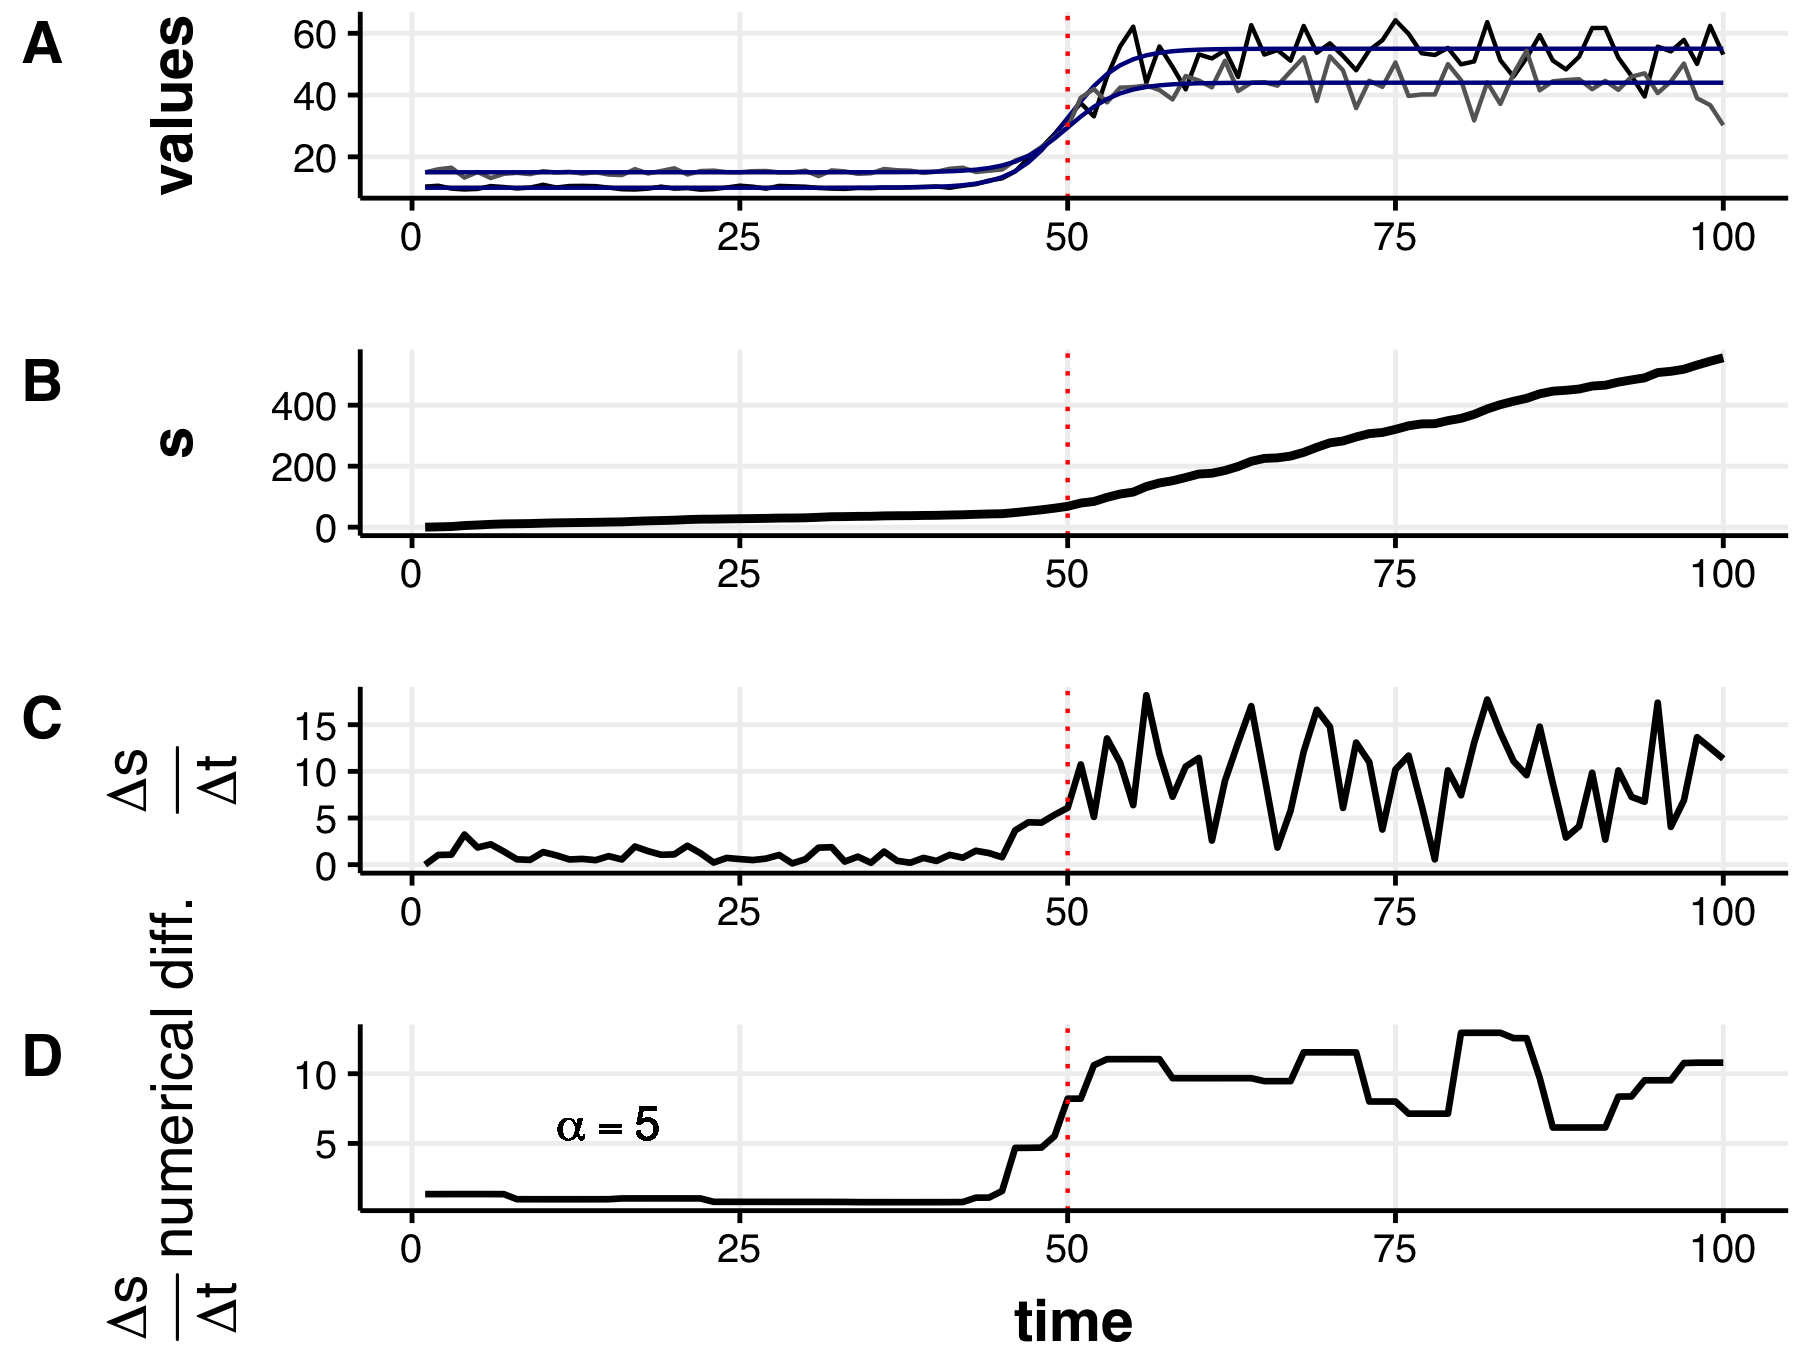
\includegraphics[width=0.65\linewidth]{E:/GitHub/myDissertation/chapterFiles/velocity/figsCalledInDiss/changeMuVarBoth_tanhAlpha0.25-5tvdiffAlpha-1000iter_stackTvdiff} 

}

\caption{The velocity signals a shift when both variables undergo shifts in the mean and variance under a slightly abrupt transition ($lpha_{tanh}=0.25$). True and observed values of $x_i$ (panel A), observed distance travelled ($s$, panel B), observed velocity (C), and the smoothed velocity (D). }\label{fig:muVarBoth.25}
\end{figure}
\begin{figure}

{\centering 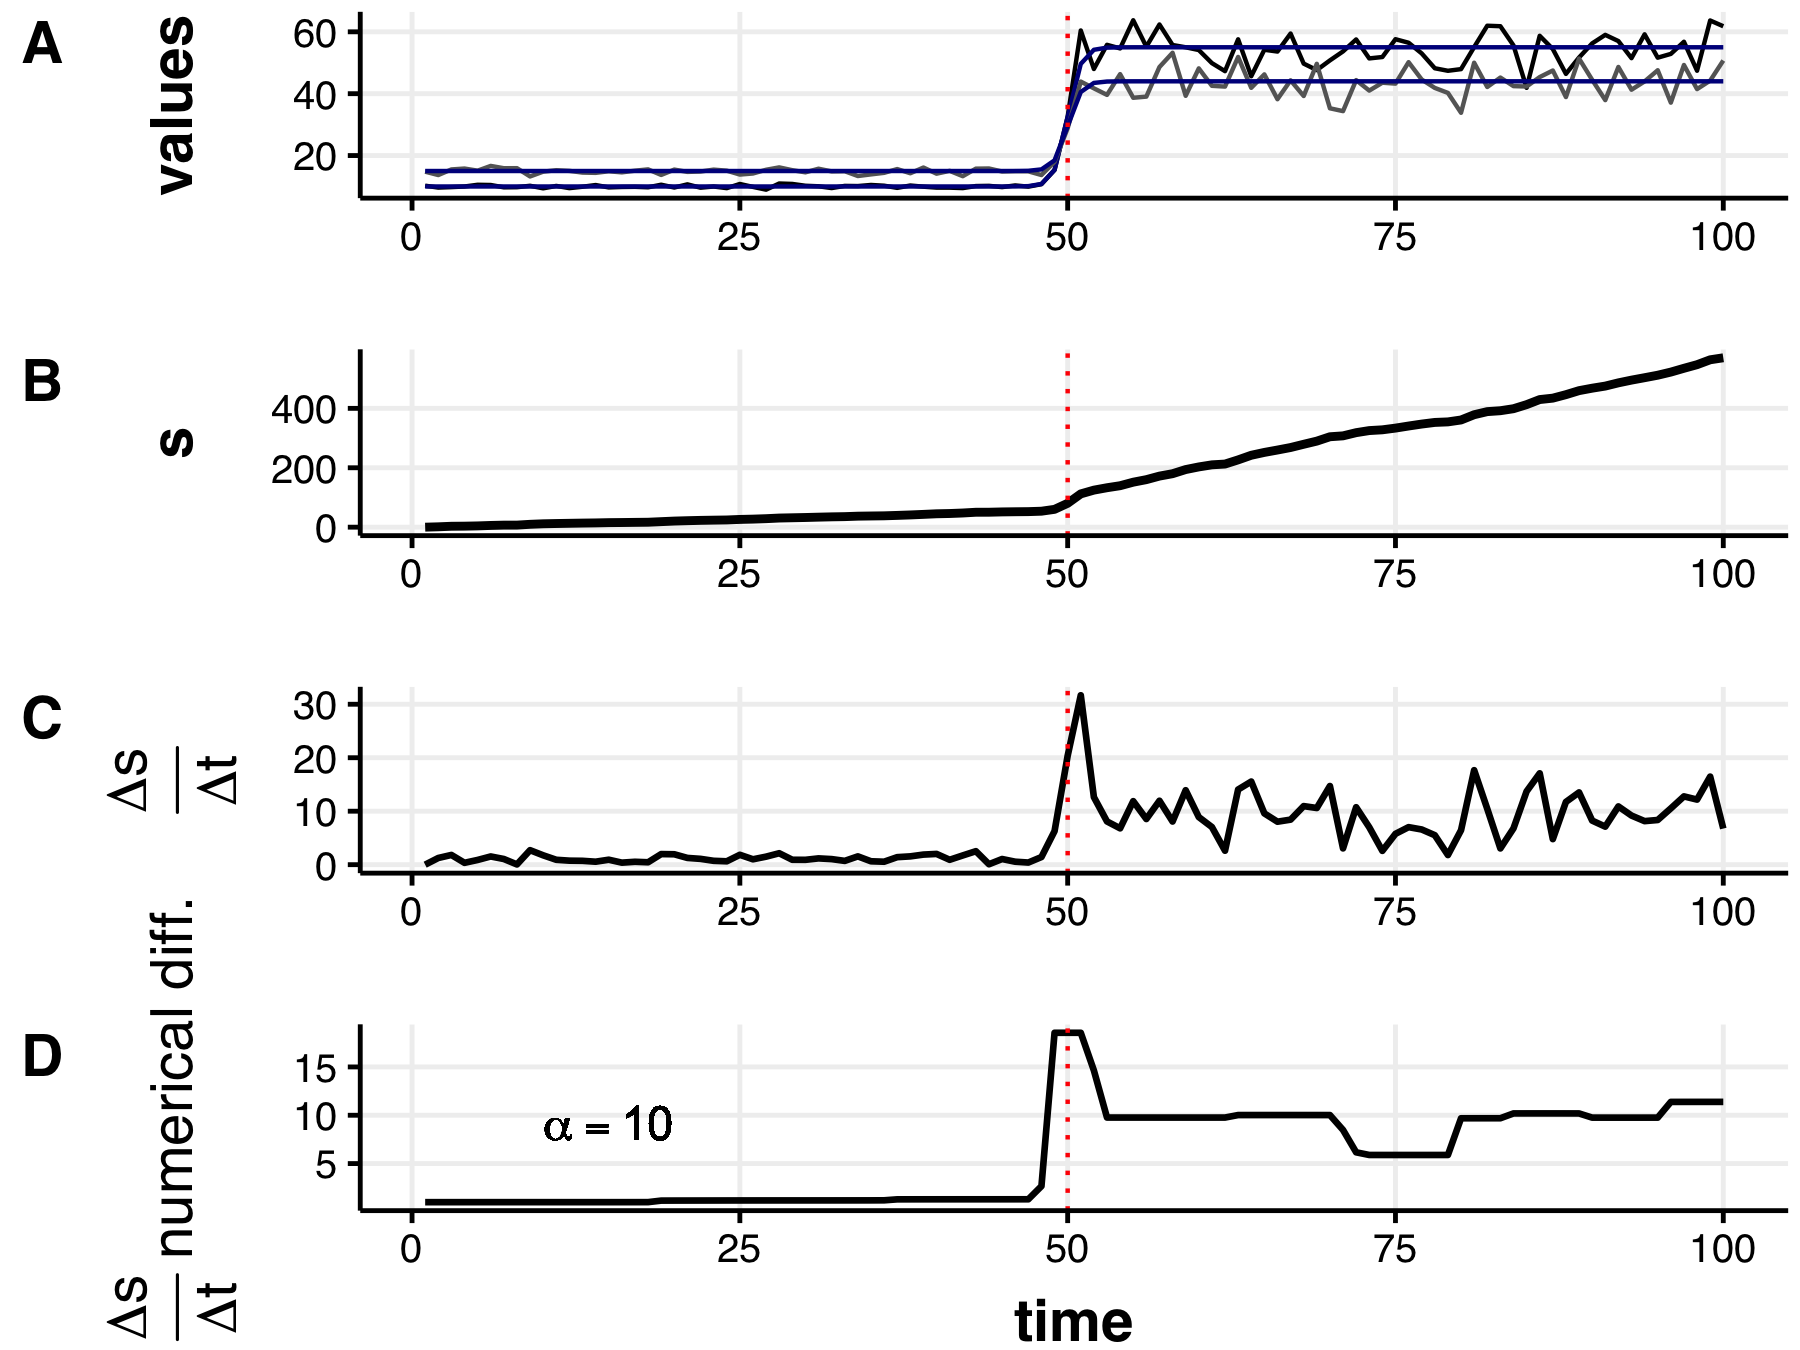
\includegraphics[width=0.65\linewidth]{E:/GitHub/myDissertation/chapterFiles/velocity/figsCalledInDiss/changeMuVarBoth_tanhAlpha1-10tvdiffAlpha-1000iter_stackTvdiff} 

}

\caption{The velocity signals a shift when both variables undergo shifts in the mean and variance under a slightly abrupt transition ($lpha_{tanh}=1.00$). True and observed values of $x_i$ (panel A), observed distance travelled ($s$, panel B), observed velocity (C), and the smoothed velocity (D). }\label{fig:muVarBoth1}
\end{figure}

\hypertarget{velocity-performance-under-empirical-transitions-paleolithic-freshwater-diatom-community}{%
\subsection{Velocity performance under empirical transitions:
paleolithic freshwater diatom
community}\label{velocity-performance-under-empirical-transitions-paleolithic-freshwater-diatom-community}}

\begin{figure}

{\centering 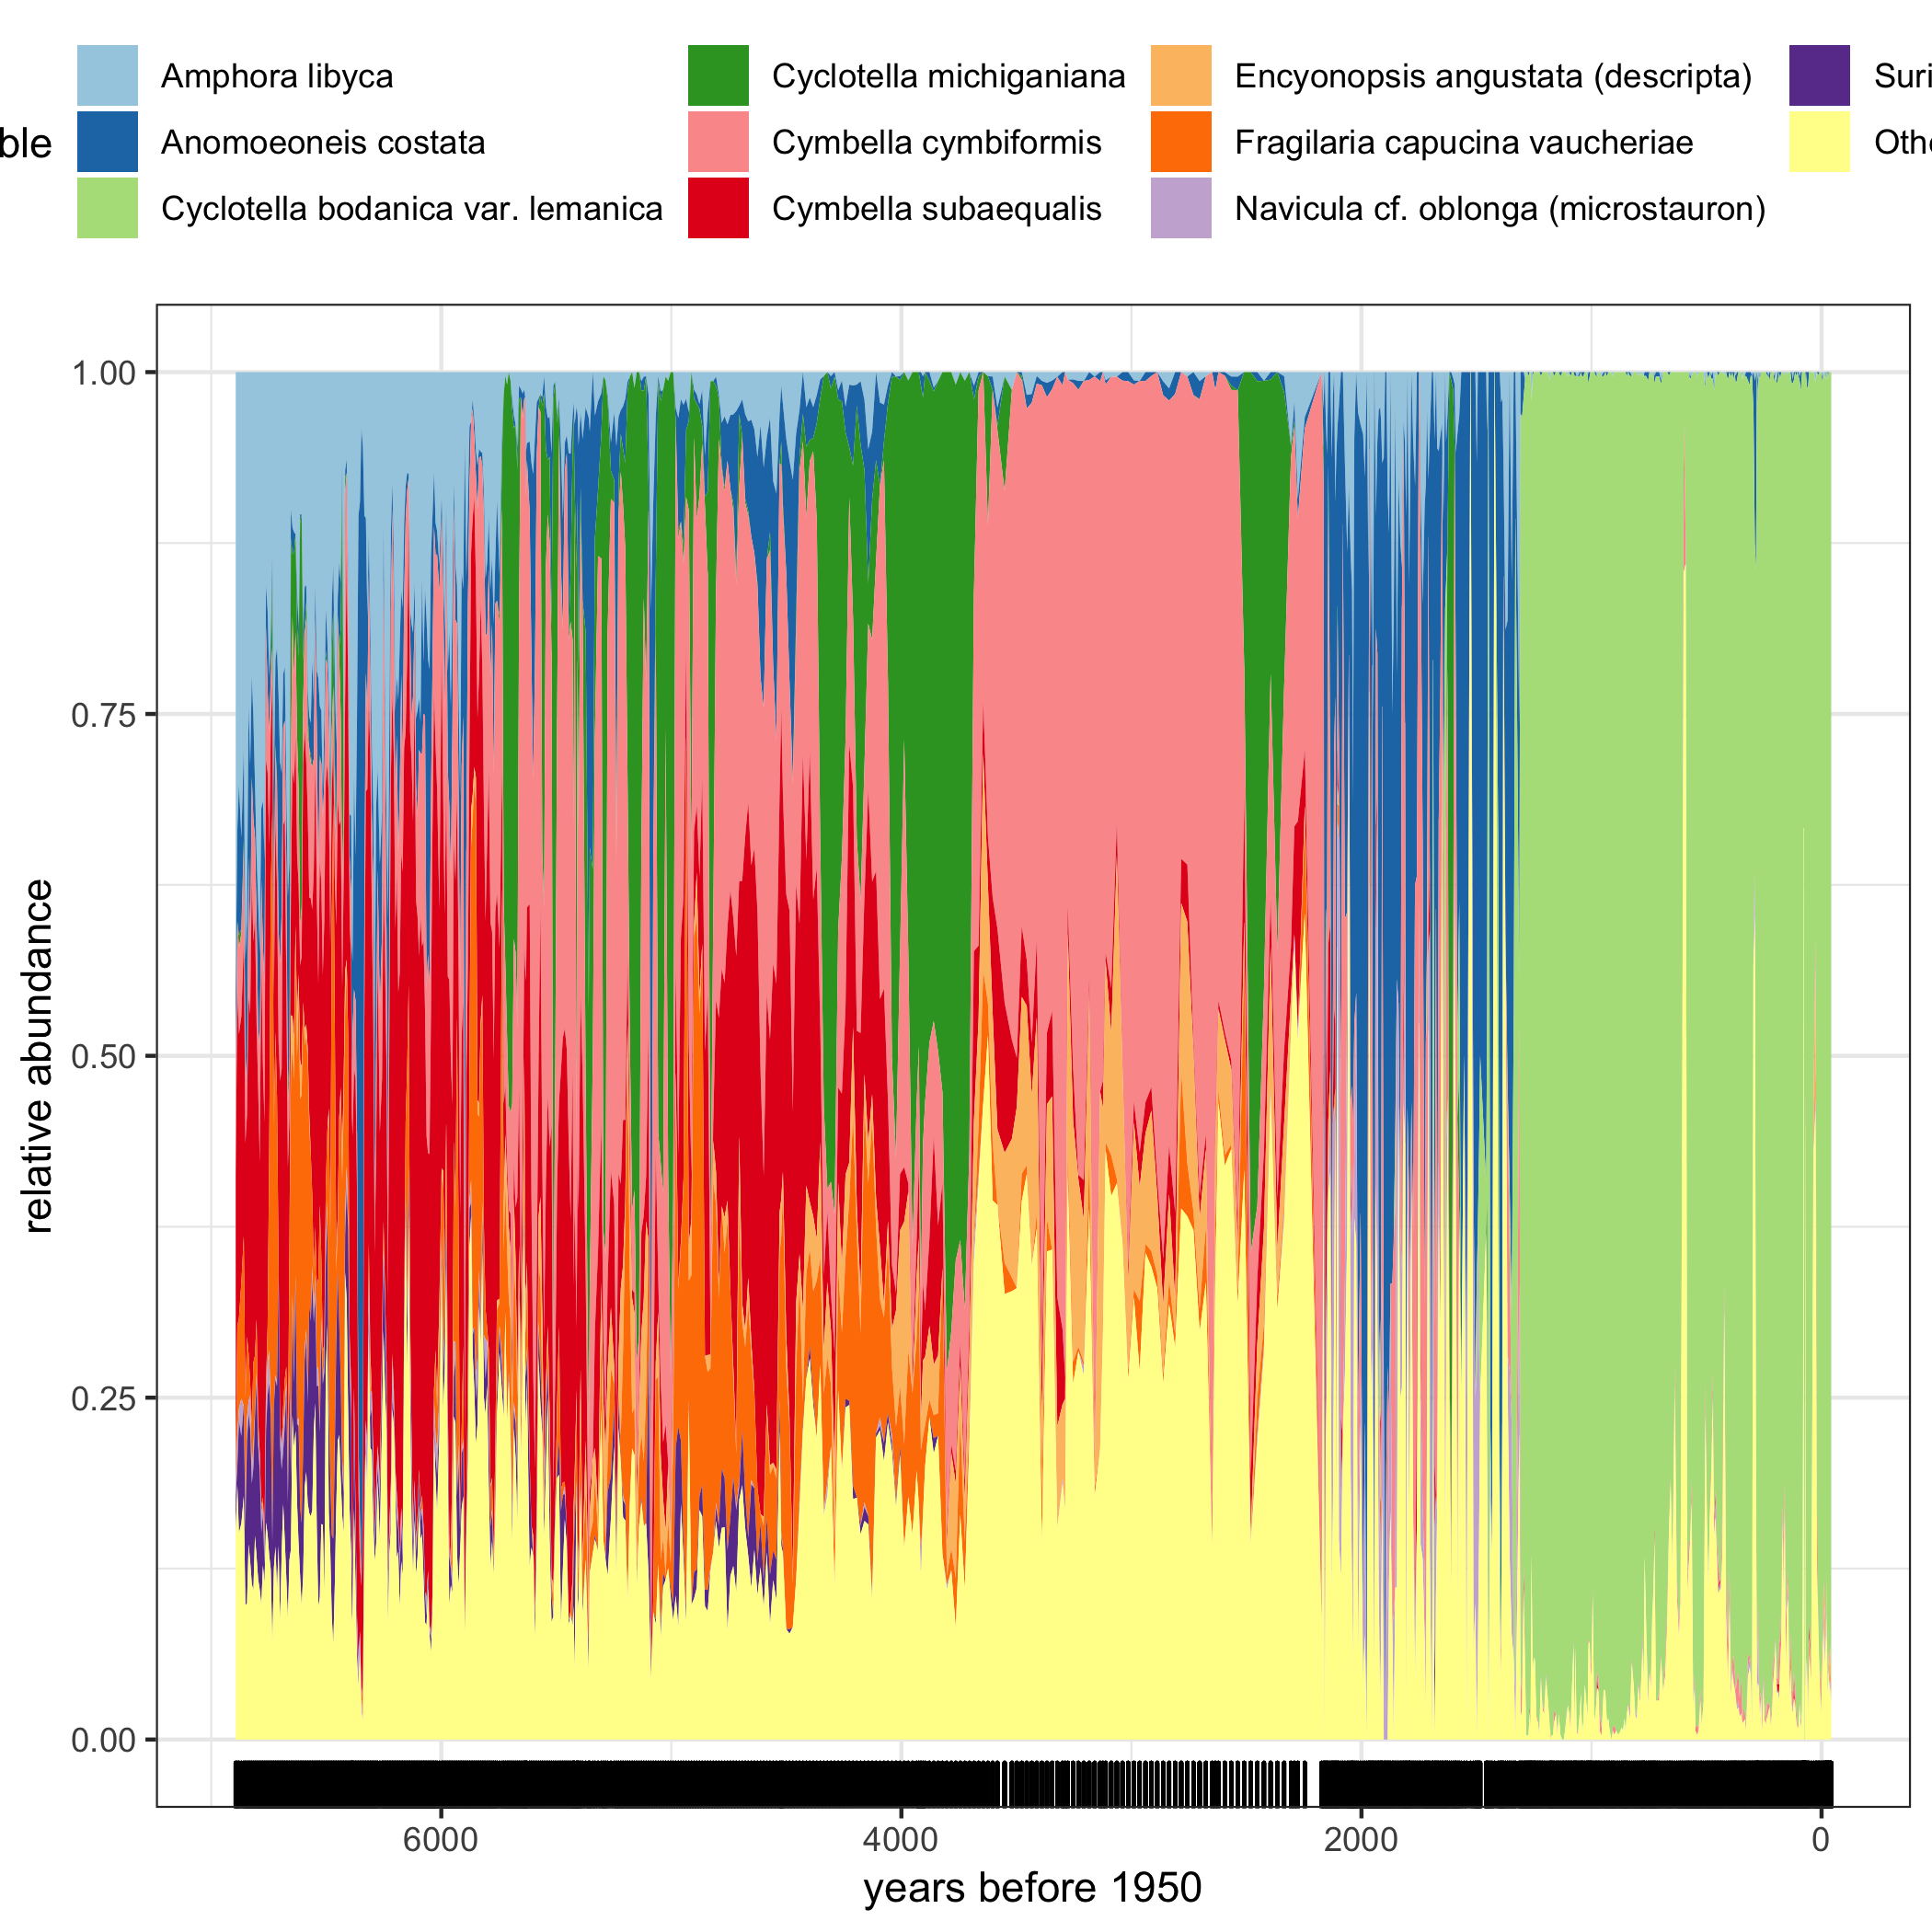
\includegraphics[width=0.65\linewidth]{E:/GitHub/myDissertation/chapterFiles/velocity/figsCalledInDiss/paleoTurnover} 

}

\caption{Relative abundances of the most common diatom species in the time series. Few species dominate the data over the entire time series, and turnover is apparent at multiple observations.}\label{fig:paleoTurnover}
\end{figure}

To gather baseline information on the use of velocity in empirical
systems data, I calculated velocity for the paleodiatom system described
in Chapter @ref(resampling) (see also Appendix @ref(appPaleo). Briefly,
the paleodiatom community comprises 109 time series over a period of
approximately 6936 years (Fig. @ref(fig:paleoTurnover)). As elaborated
in @spanbauer\_prolonged\_2014, the paleodiatom community is suggested
to have undergone regime shifts at multiple points. These abrupt changes
are apparent when exploring the relative abundaces over time, as there
are extreme levels of species turnover at multiple points in the data
(Fig. @ref(fig:paleoTurnover)). Using Fisher Information and
climatological records, @spanbauer\_prolonged\_2014 suggest that regime
shifts in this system at approximately 1,300 years before present (where
present is equal to year 1950).

\begin{figure}

{\centering 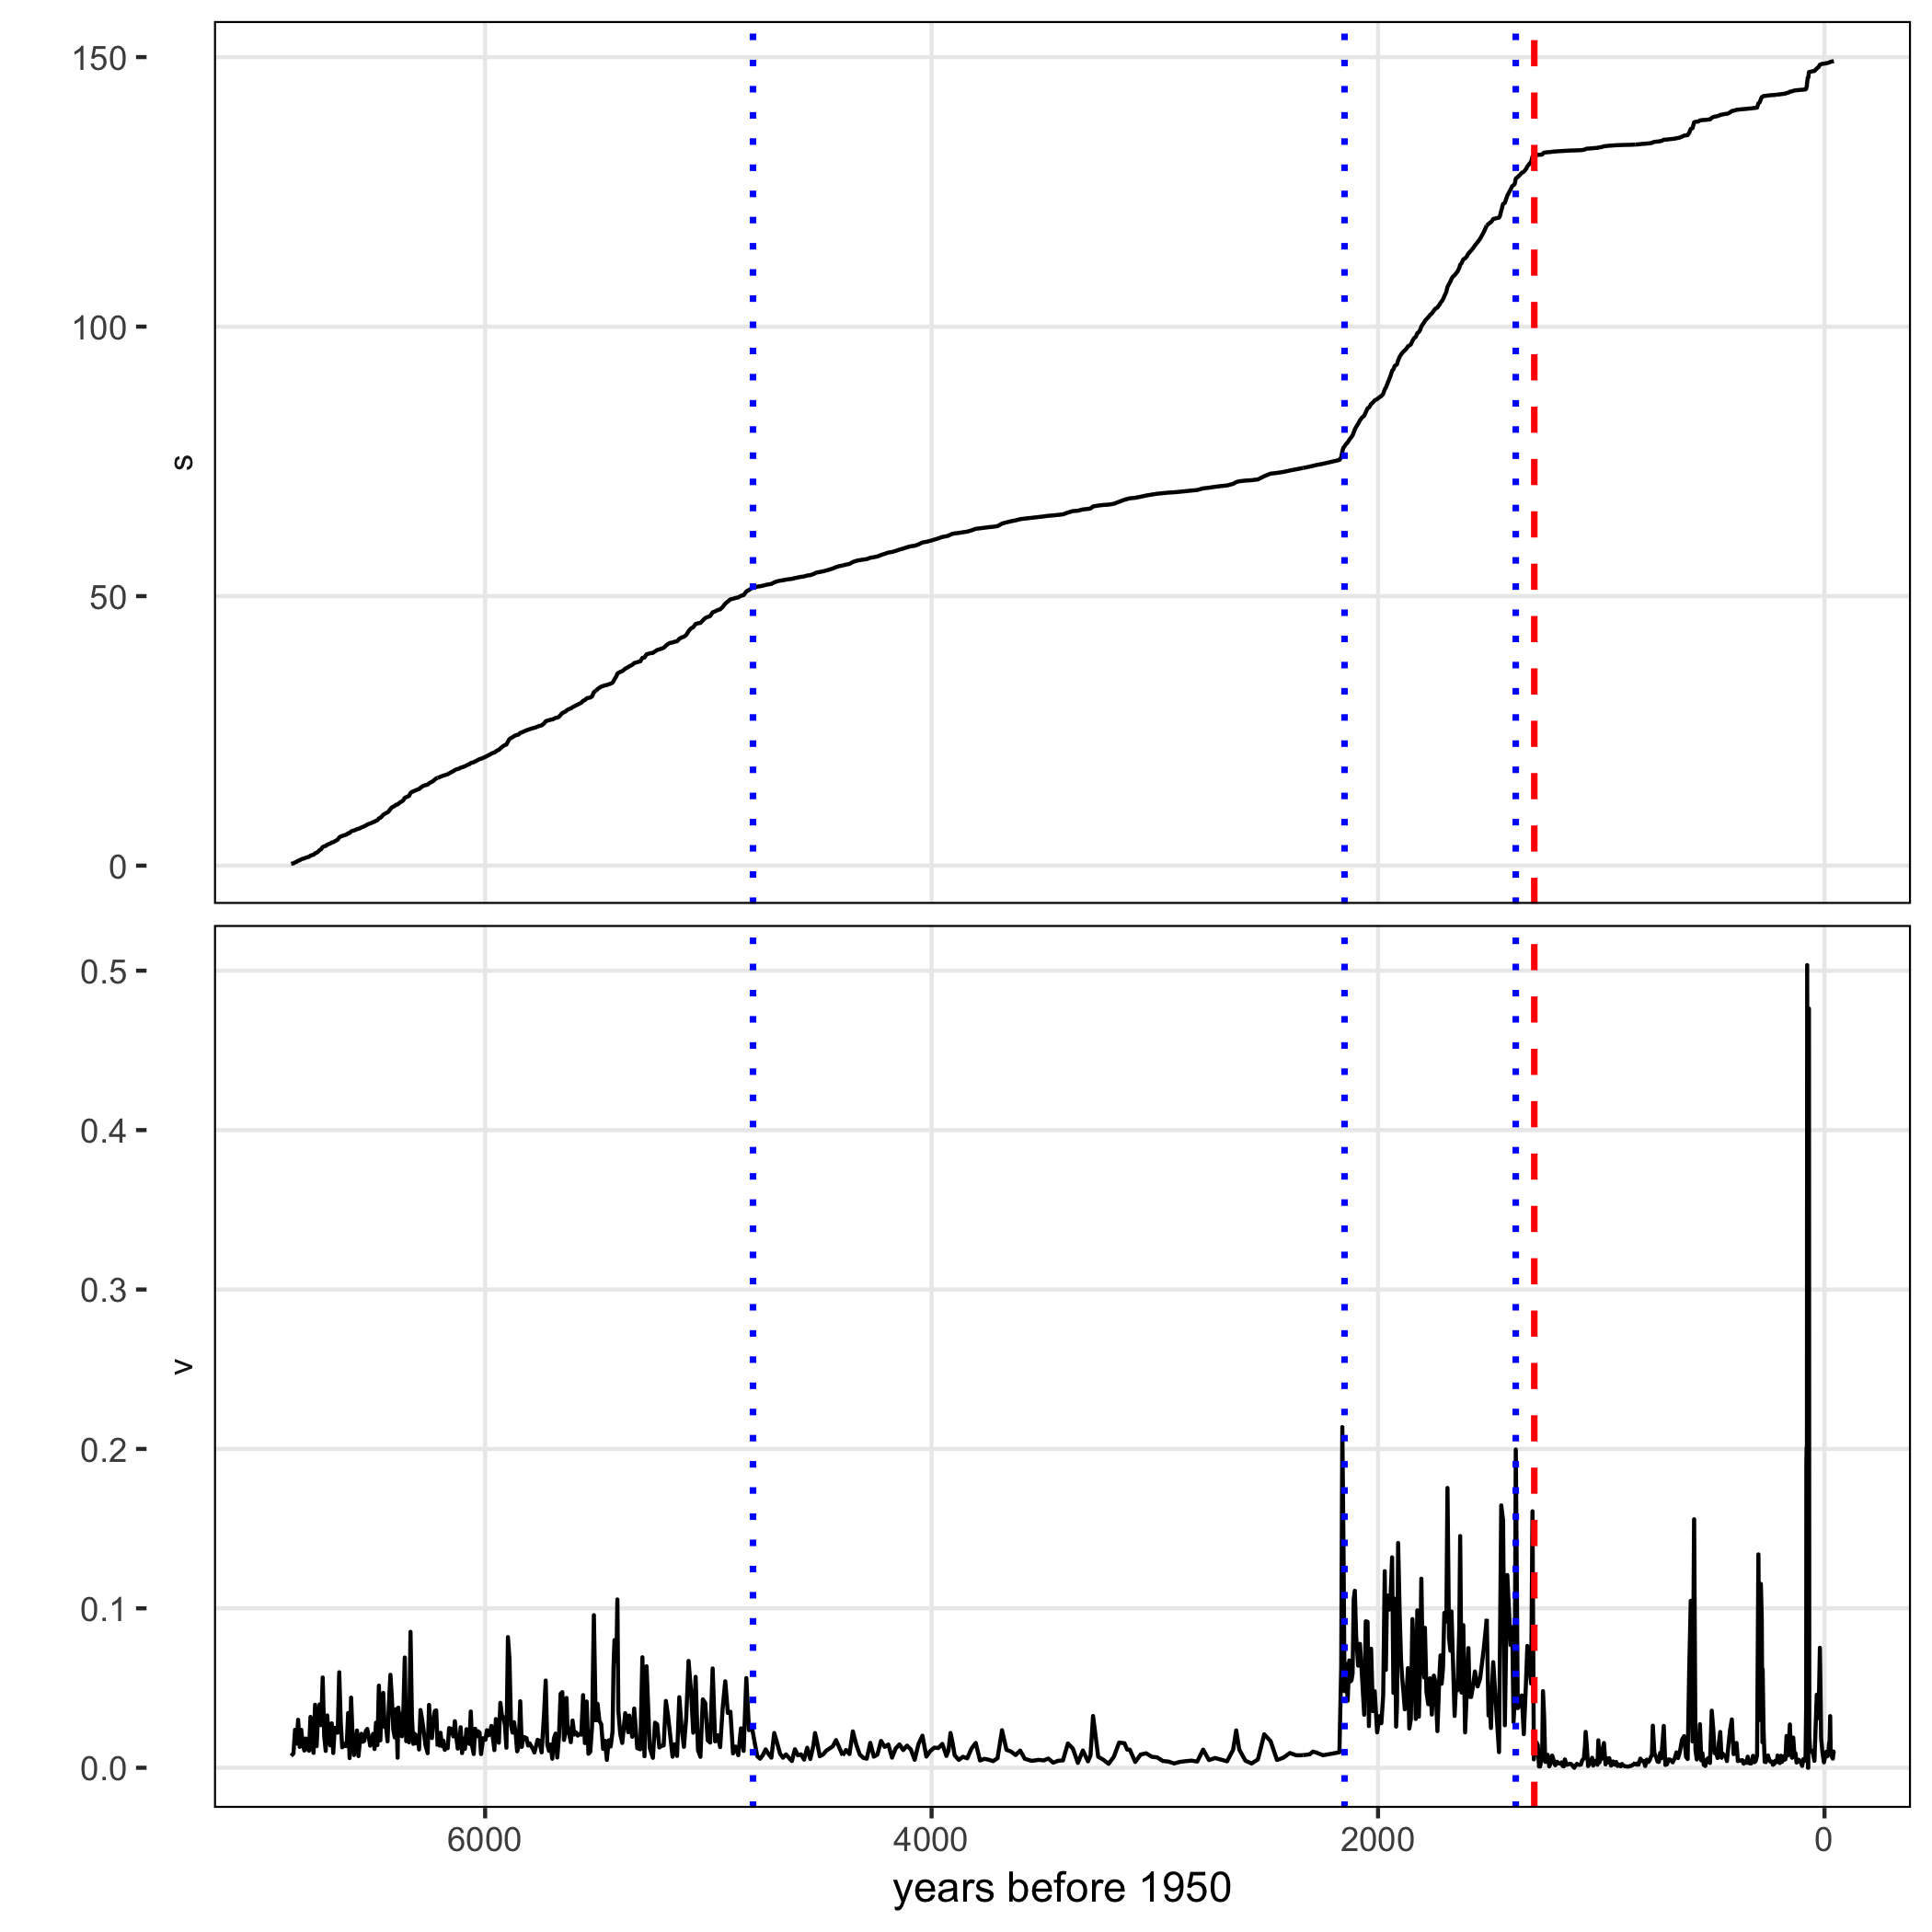
\includegraphics[width=0.65\linewidth]{E:/GitHub/myDissertation/chapterFiles/velocity/figsCalledInDiss/paleoVelocity} 

}

\caption{Velocity $v$ and distance travelled $s$ of the paleodiatom time series. Dashed line at 1,300 years before 1950 indicates the regime shift identifed in Spanbauer et al. (2014). Dotted lines indicate regime shifts as visually identified on metrics $s$ and $v$.}\label{fig:paleoVelocity}
\end{figure}
\begin{figure}

{\centering 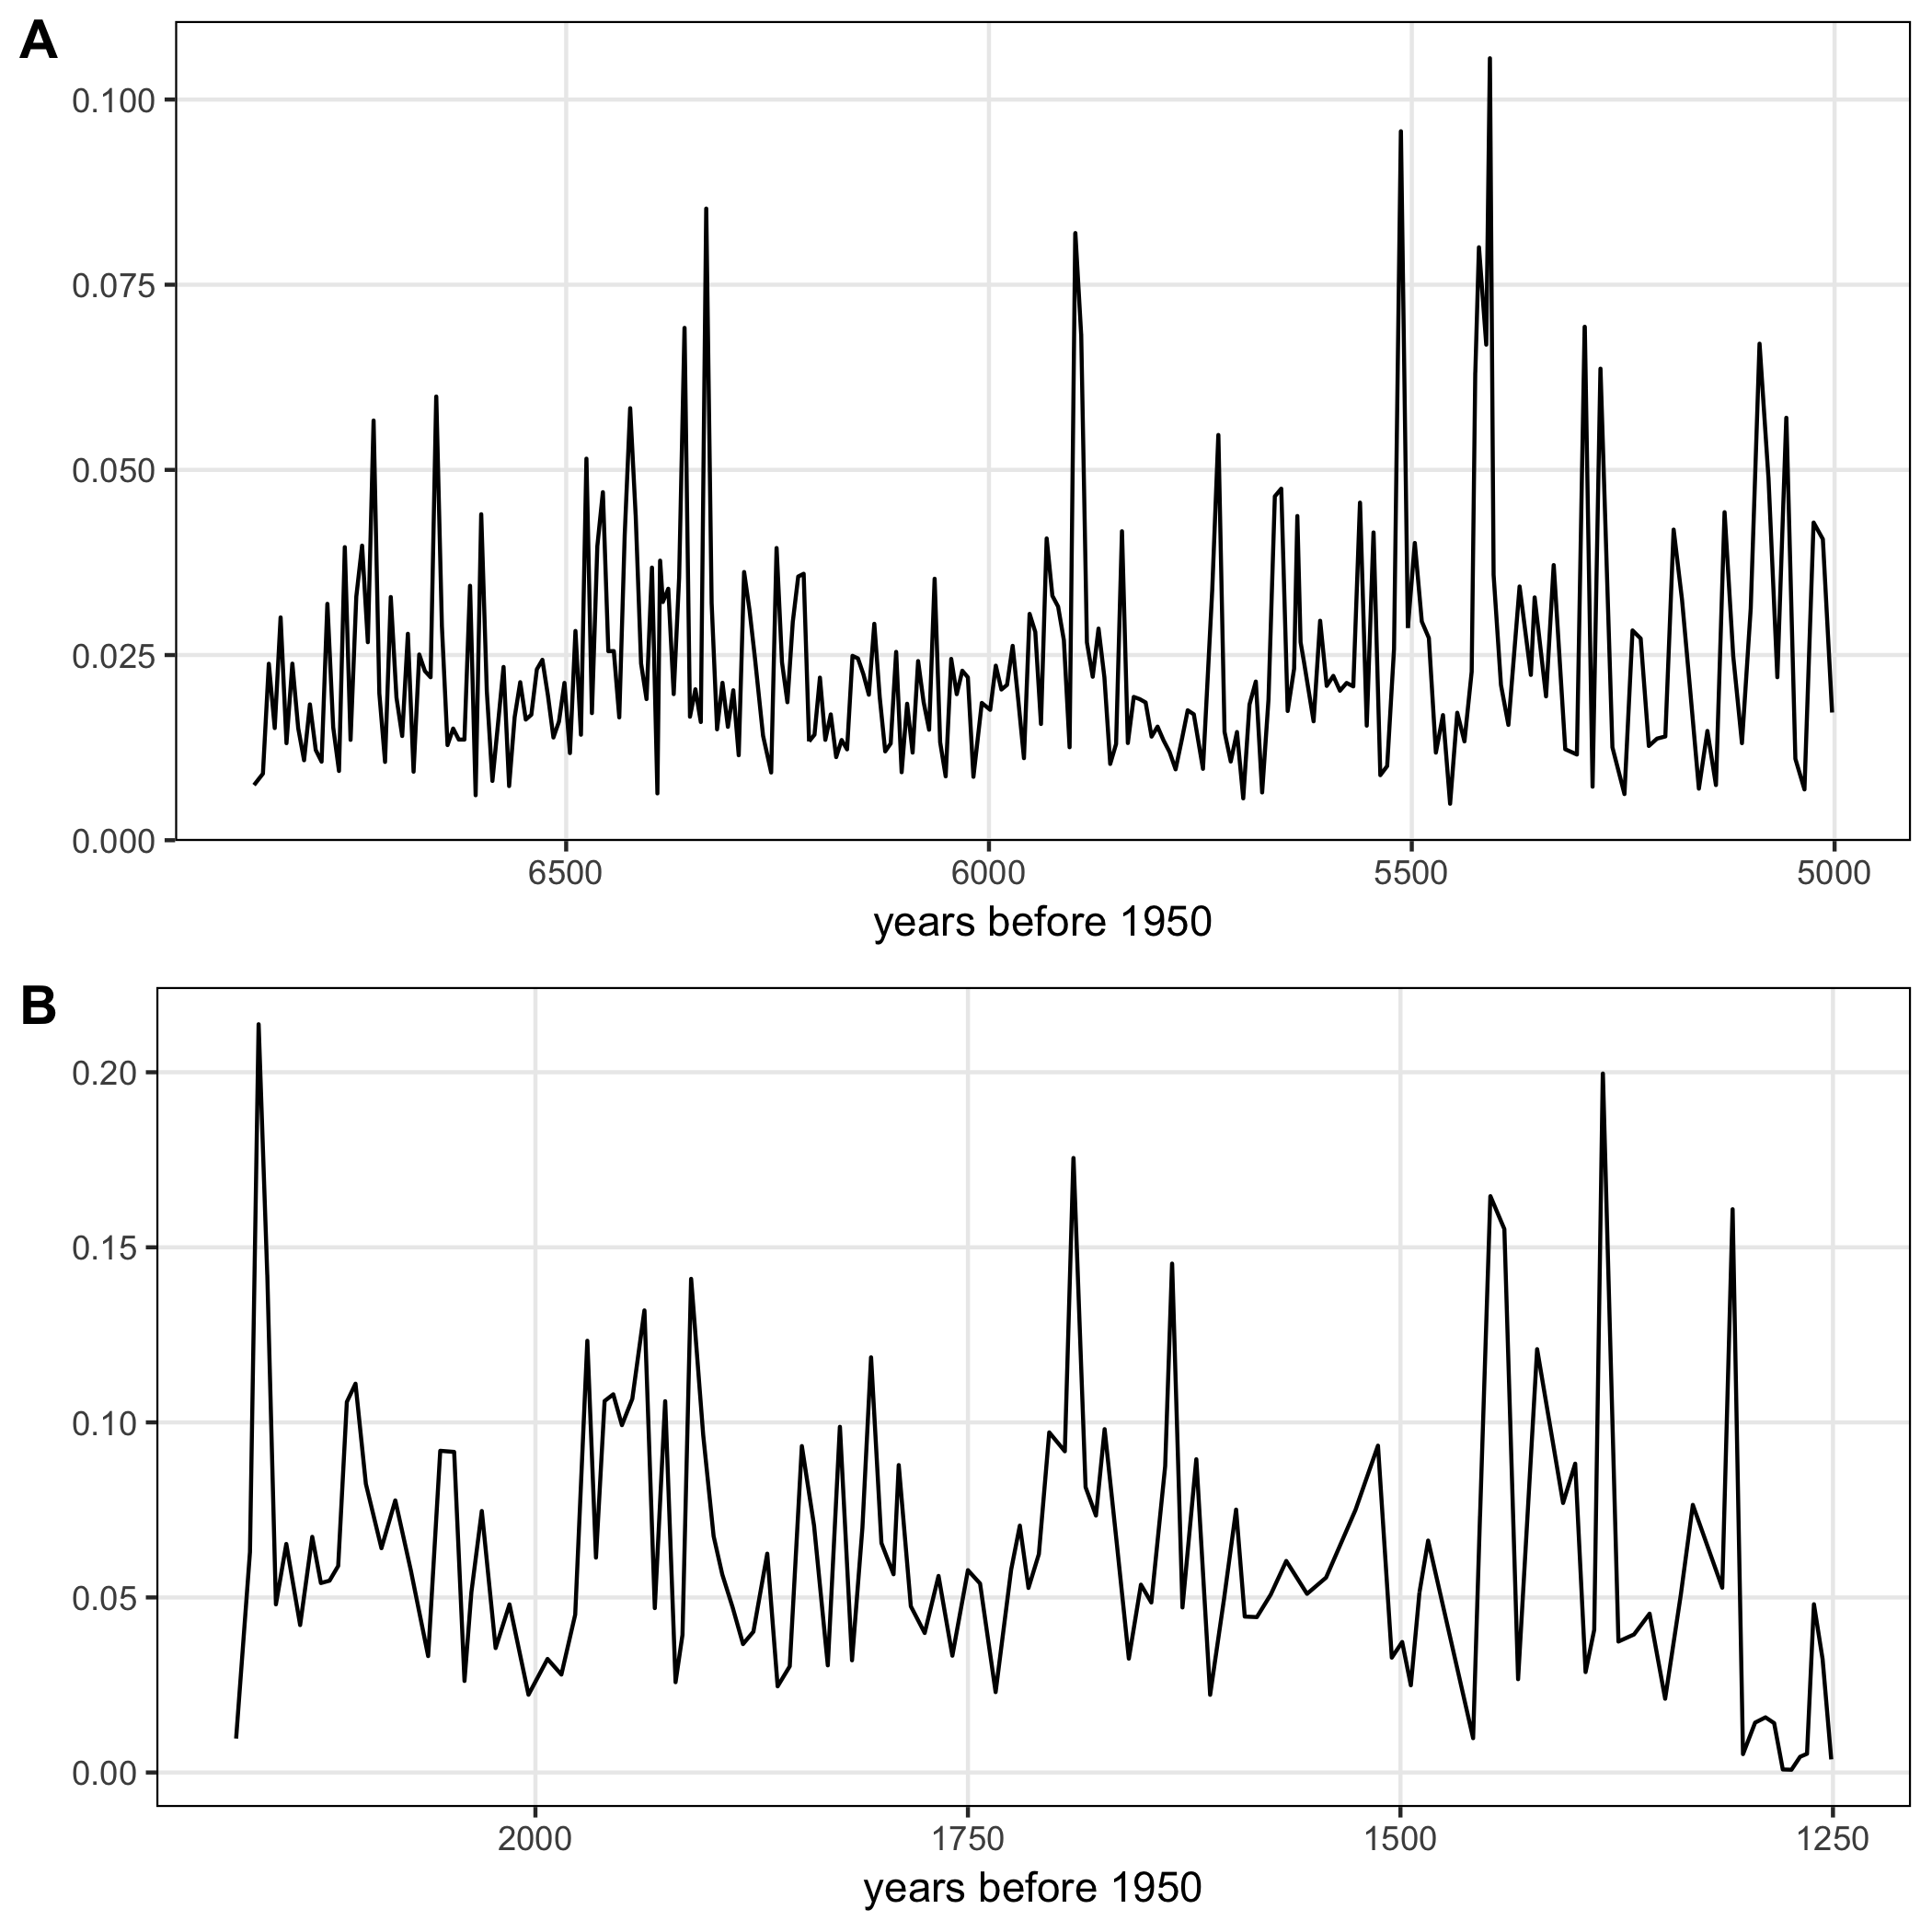
\includegraphics[width=0.65\linewidth]{E:/GitHub/myDissertation/chapterFiles/velocity/figsCalledInDiss/paleoRegime1and3} 

}

\caption{Velocity ($v$) indicates periodic-like conditions in the first (A) and second (B) regimes.}\label{fig:paleoRegime1and3}
\end{figure}

@spanbauer\_prolonged\_2014 used different regime detection metrics
coupled with regional climatological events to identify regime shifts in
the system, suggest that a regime shift occurred at
\textasciitilde{}1,300 years before present. Using the methods outlined
above, I calculated the distance travelled (\(s\)) and velocity (\(v\);
Fig. @ref(fig:paleoV)). The results of \(v\) and \(s\)
(@ref(fig:paleoVelocity)) on the relative abundance data correspond with
both the large shifts in species dynamics (see Fig
@ref(fig:paleoTurnover), and also with the regime shift identified by
@spanbauer\_prolonged\_2014. However, two primary results can be made
from the metrics \(v\) and \(s\) that are not obvious nor identified
numerically in the results of @spanbauer\_prolonged\_2014 (): 1. Two
additional large shifts occurred at approximately 2,500, 4,800 and years
before 1950\\
1. The periods before the first and after the second large shifts appear
oscillatory (Fig. @ref(fig:paleoRegime1and3)).\\
To determine whether removing the noise in the data, I interpolated the
each time series using function \texttt{stats::approx} to 700 time
points. Next, I calculated the distance travelled of the entire system,
\(s\). Finally, I obtained the derivative of \(s\) by using a
regularized differentiation (using function \texttt{tvdiff::TVRegDiffR};
parameters were \(iter = 2000\), scale = small, \(ep = 1 x 10^-6\), and
\(\alpha = 100\))\footnote{*We created the R-wrapper \texttt{tvdiff} as
  a Python wrapper for the tvdiff MatLab package @price2019tvdiff}..
This method of regularized differentiation is an ideal approach to
smoothing \(s\) because it assumes the data are non-smooth and
incorporates finite differencing.

\begin{figure}

{\centering 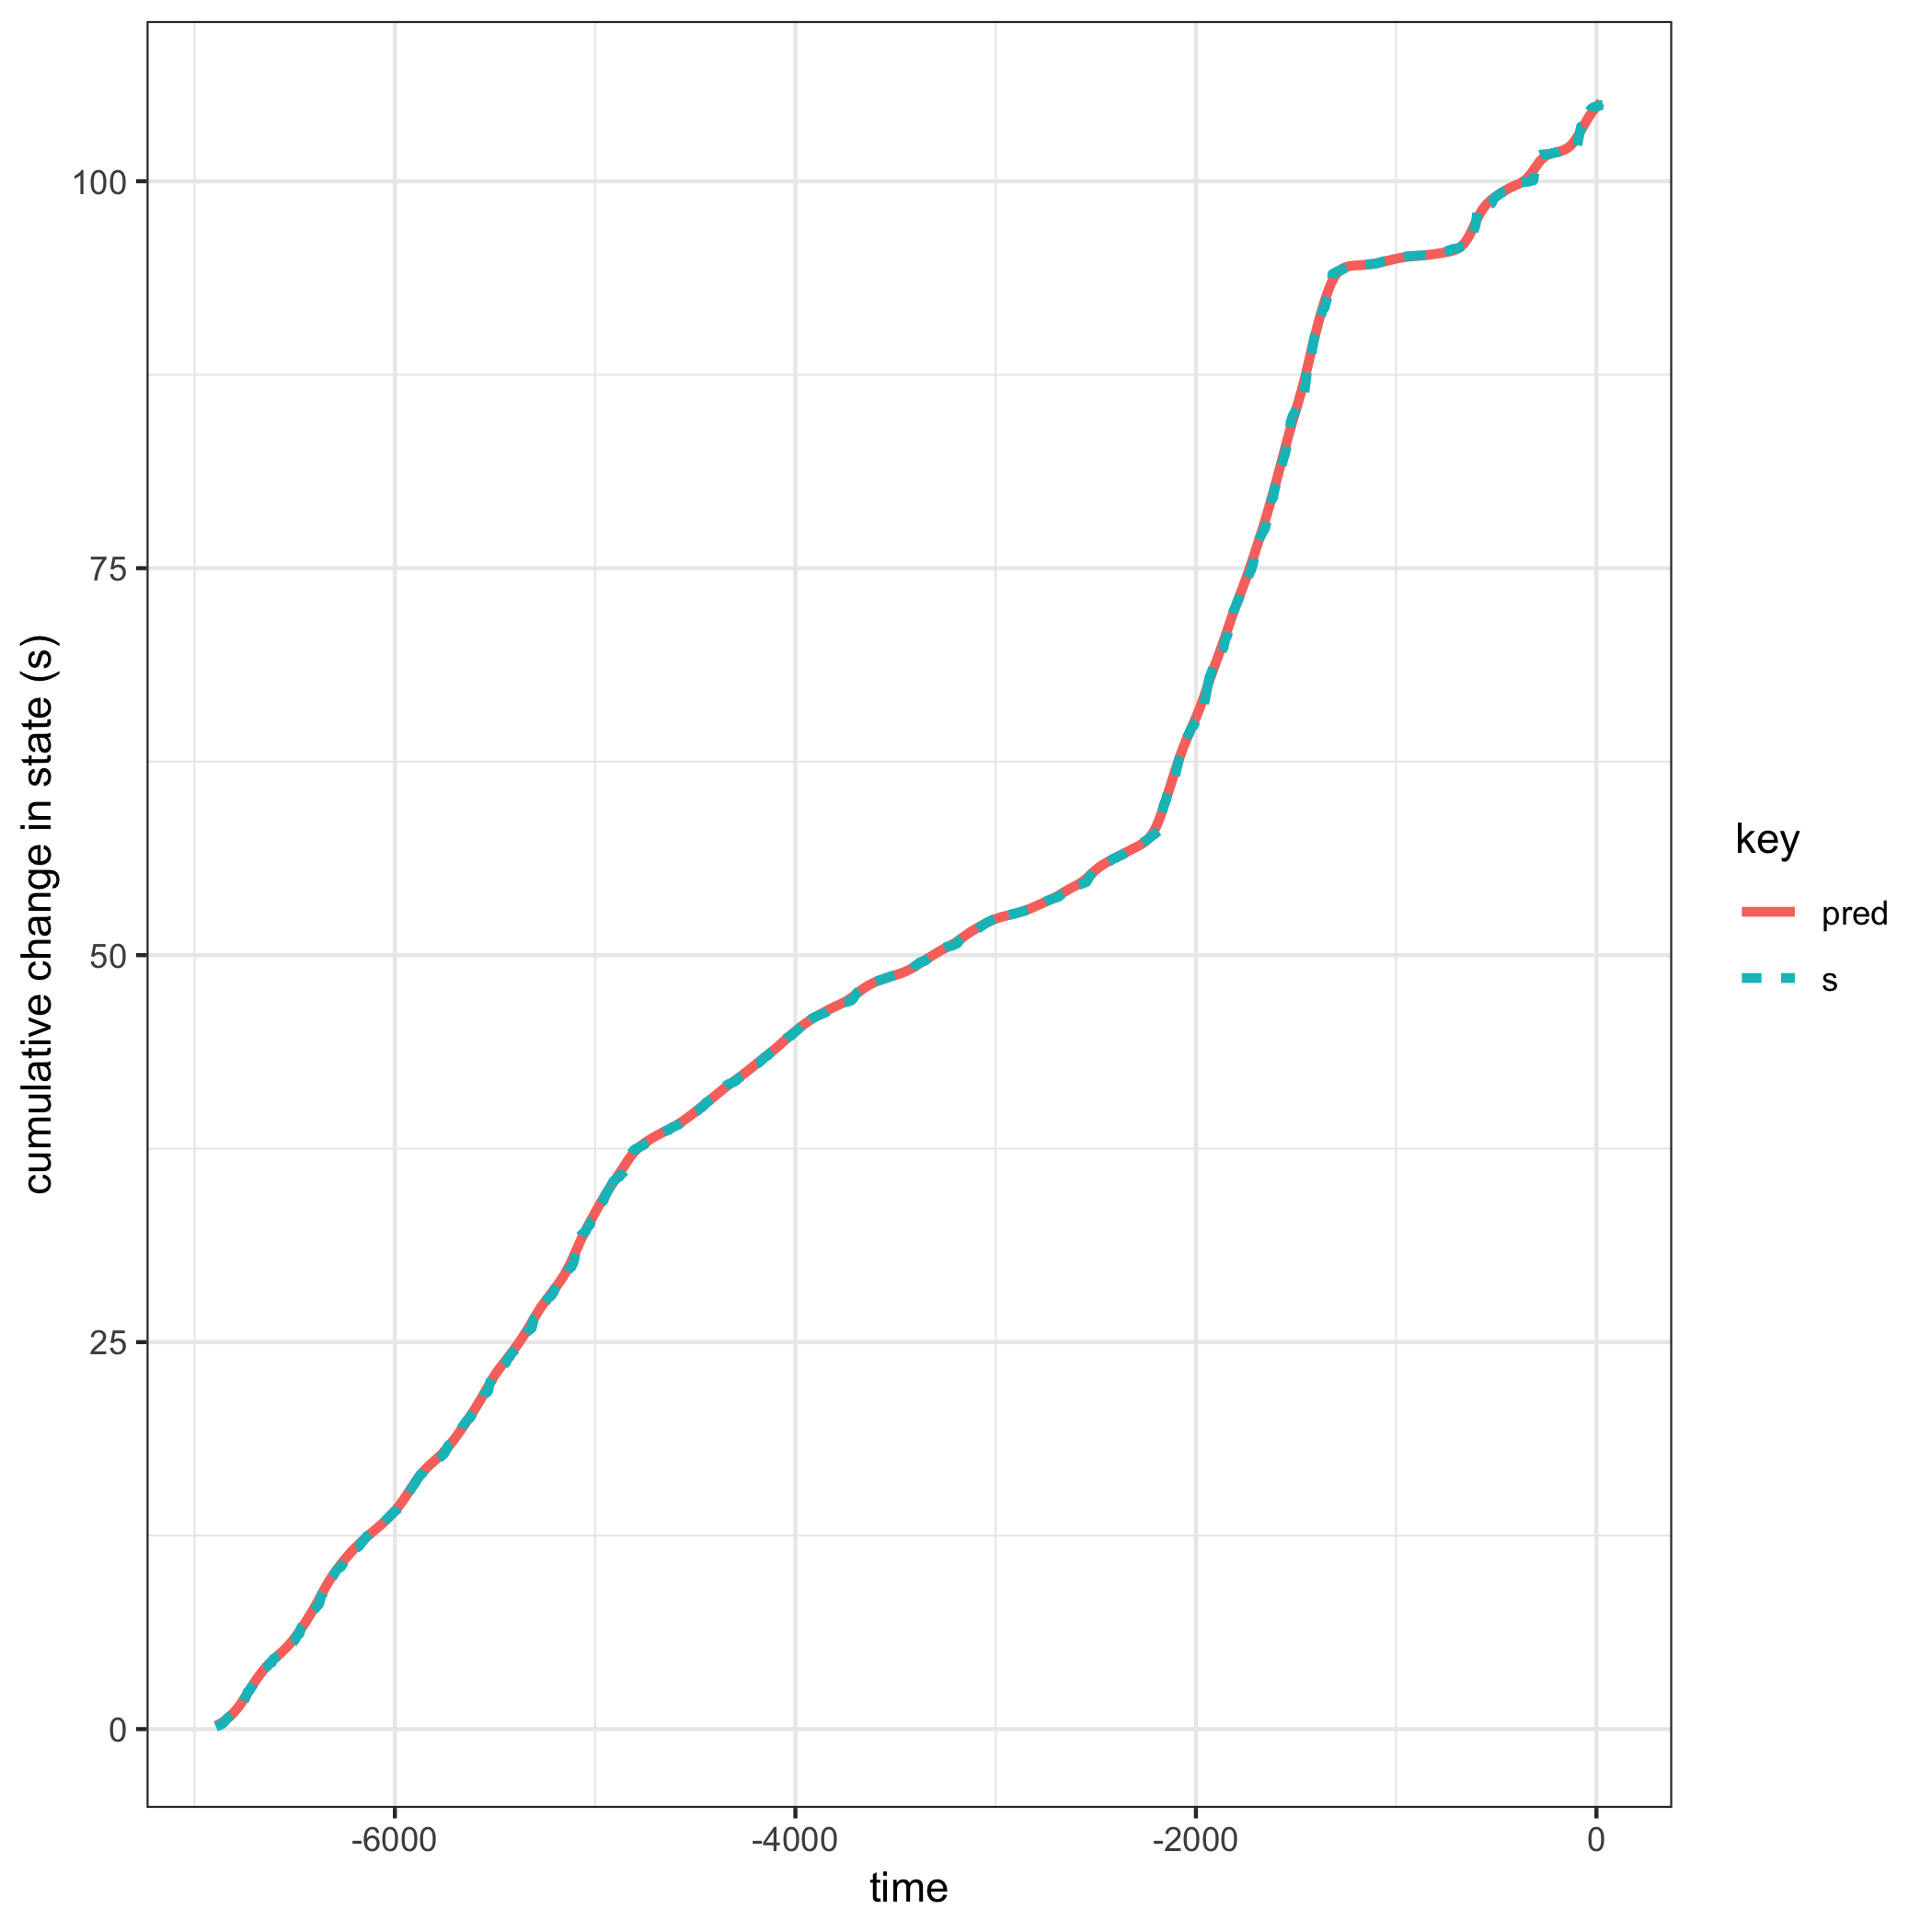
\includegraphics[width=0.65\linewidth]{E:/GitHub/myDissertation/chapterFiles/velocity/figsCalledInDiss/paleoObsPred} 

}

\caption{The regularized differentiation of $s$ was best fit using $\alpha = 100$. Higher overlap of $s$ and pred indicates a good fit of the regularized differentiated metric to the non-smoothed metric, $s$.}\label{fig:paleoObsPred}
\end{figure}

The smoothed velocity (@ref(fig:paleoV)) provides a similar but smoother
picture of the velocity of the system trajectory. Comparing the smoothed
(@ref(fig:paleoV)) to the non-smoothed velocity
(@ref(fig:paleoVelocity)) yields similar inference regarding the
location of the regime shifts at 2,200 and 1,300 years before present,
however, it more clearly demonstrates potential inter-regime dynamics
(e.g., between 7,000 and 4,800 years before present), which were not
identified in previous study of this ssytem
{[}@spanbauer\_prolonged\_2014{]}.

\begin{figure}

{\centering 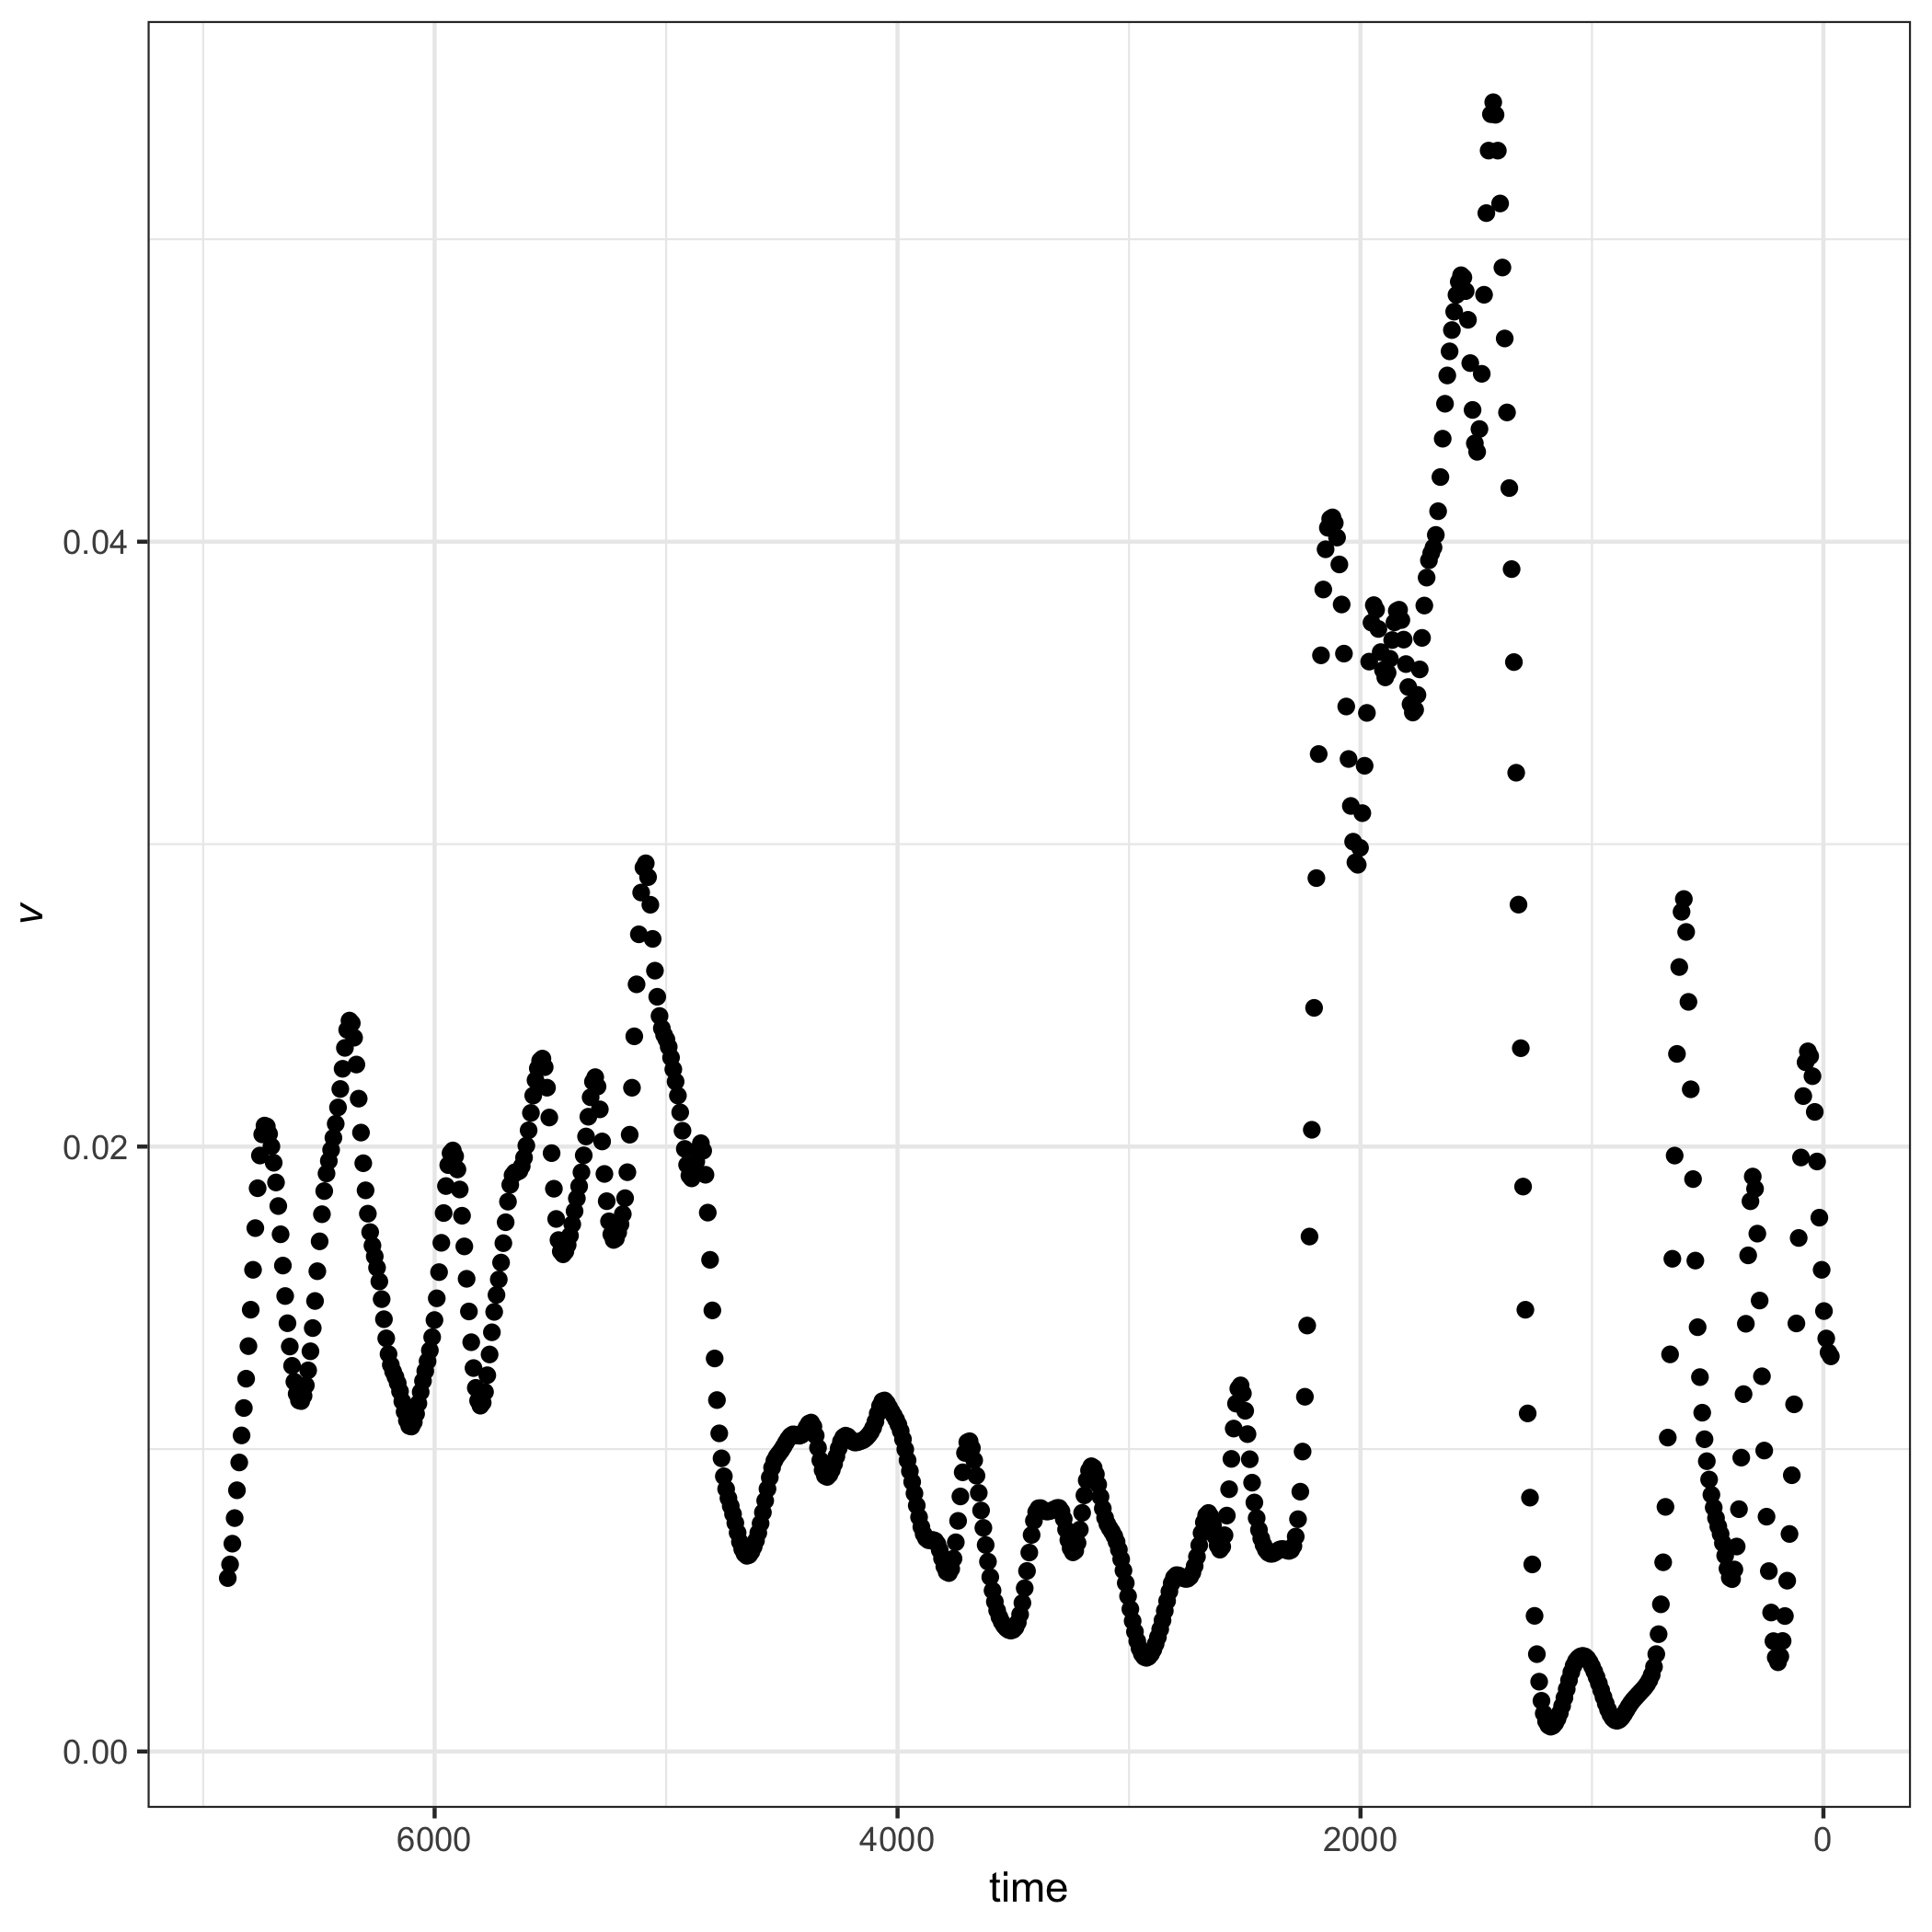
\includegraphics[width=0.65\linewidth]{E:/GitHub/myDissertation/chapterFiles/velocity/figsCalledInDiss/paleoV} 

}

\caption{The velocity metric  ($v$) signals potential periodicities in the paleo diatom time series data when the distance travelled metric, $s$, is smoothed using regularized differentiation methods [@price2019tvdiff].}\label{fig:paleoV}
\end{figure}

\hypertarget{discussion}{%
\subsection{Discussion}\label{discussion}}

Here, I described the steps for calculating a novel regime detection
metric, system velocity (\(v\)). First described in @fath\_regime\_2003,
\(v\) is used as a single step for caclulating a more complicated regime
detection metric, Fisher Information (see also Chapter @ref(fiGuide)).
System velocity is arguably simple to calculate, as shown in this
chapter, captures the total change in system variables under a variety
of mean and variance conditions. The metric does not, however, perform
well as variance increases (Fig. @ref(simVarPlot2)), and smooothing the
original data does not reduce the noise surrounding this metric when
variance is moderate (Fig. @ref(smoothV)). Variance is a commonly-used
indicator of ecological regime shifts (@brock\_variance\_2006), however,
is difficult to interpret when the number of variables is \(\ggg\) a
few. System velocity, \(v\), may be useful in situations where the
number of state variables is \(\ggg\) few, and appears especially useful
when the magnitude of change in one or more state variables is high
(Figs. @ref(fig:simVplot2),@ref(fig:muBoth.75)). For example, this
method will likely identify signals of regime shifts where the shift is
defined as high species turnover within a community (Fig.
@ref(fig:muVarBoth1)).

This study provides baseline expectations of the velocity of the
distance travelled, \(V\), as an indicator of abrupt change in a
multivariable system. Although a useful first step, this metric should
next be critiqued in a sensitivity analytical approach, where a
statistical measure is used to determine whether \(V\) indicates abrupt
shifts prior to occurrence (c.f. during or after), particularly with
respect to its performance in community-level empirical data. The
paleolitic diatom data used in the last section of this chapter is also
presented in the documentation for my R Package,
\textbf{regimeDetectionMeasures} (Appendix @ref(appPaleo)). In this case
study, the `distance travelled', \(s\) (Eq. @ref(eq:diffXsq2)), clearly
exhibits shifts at points where expert opinion and species turnover (in
species dominance) agree that a large change occurred. Further,
velocity, \(v\) (see \emph{dsdt} in package materials) indicates a large
shift at only the most predonimnant shift in the time series, perhaps
due to the metric's sensitivity to variance (Fig. @ref(fig:simVplot2).

Further work is required to determine the utility of system velocity as
a regime detection metric, however, this chapter demonstrates that the
metric may indicate clear shifts in variable means and variability about
the means. In addition to examining high-dimensional and noisy data, a
study of the performance of \(v\) under conditions where few variables
exhibit large changes while many variables are relatively constant may
also prove useful. Additionally, this metric may be a useful tool for
reducing the dimensionality of high dimensional data. Although the
metric loses much information, as opposed to some dimension reduction
techniques, e.g.~Principal Components Analysis PCA, the metric is simple
to calculate (even by hand), is computationally inexpensive, and is
intuitive, unlike many clustering algorithms (e.g., Non-metric
Multidimensional Scaling NMDS). Like system velocity, methods of the
latter variety (e.g.~NMDS) require post-hoc statistical analyses to
confirm the location of clusters (or abrupt change, regime shifts),
while methods of the former variety (e.g.~PCA) retain loadings but do
not necessarily identify the locations of abrupt shifts.

\hypertarget{supplementary-figures}{%
\subsection{Supplementary Figures}\label{supplementary-figures}}

This section contains additional examples of the behavior of velocity,
\(v\) when varying the mean and/or variance prior to and/or after the
induced abrupt shiftt in the toy system with a discontinuous transition
at \(t=50\).

\begin{figure}

{\centering 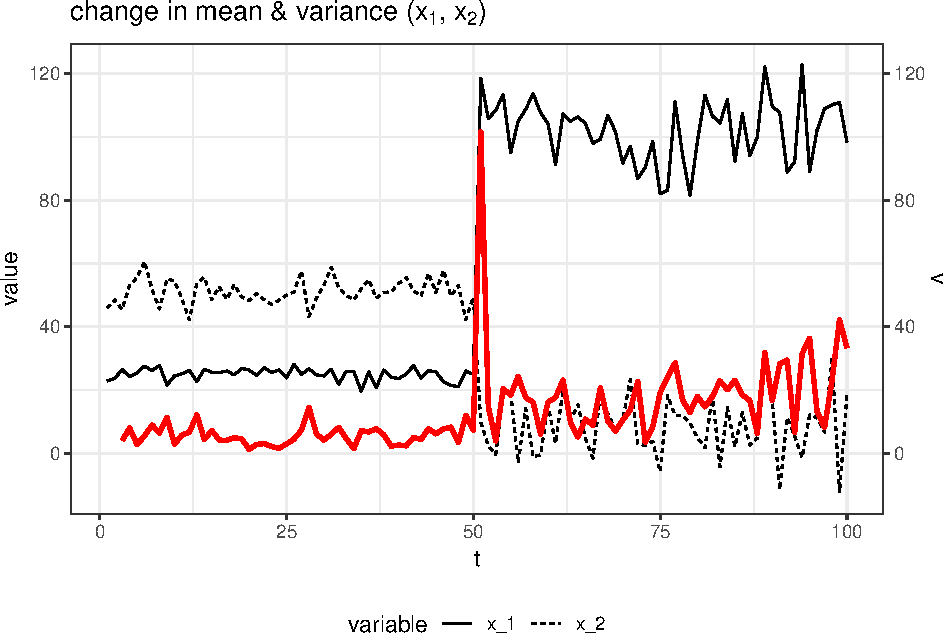
\includegraphics[width=0.65\linewidth]{06-chap-velocity_files/figure-latex/velocSysEx2-1} 

}

\caption{System change ($s$) and velocity ($v$) of the model system over the time period. Change in means ($\bar{x}_{1_{pre}}=25$, $\bar{x}_{1_{post}}=100$, $\bar{x}_{2_{pre}}=50$, $\bar{x}_{2_{post}}=10$) and an increase in variance ($\sigma_{1_{pre}}=2$, $\sigma_{1_{post}}=10$, $\sigma_{2_{pre}}=5$,  $\sigma_{2_{post}}=10$).}\label{fig:velocSysEx2}
\end{figure}

\begin{figure}

{\centering 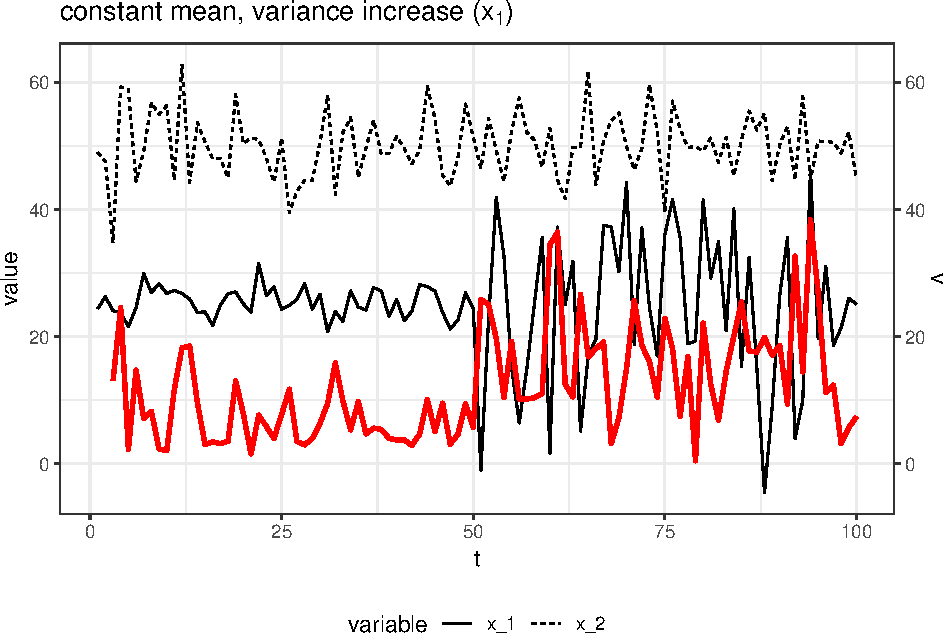
\includegraphics[width=0.65\linewidth]{06-chap-velocity_files/figure-latex/velocSysEx3-1} 

}

\caption{System change ($s$) and velocity ($v$) of the model system over the time period. Constant means ($\bar{x}_1=25$, $\bar{x}_2=50$) and sharp change in variance for one state variable $\sigma_{1_{pre}} = 2$, $\sigma_{1_{post}} = 12$, $\sigma_{2_{pre,post}} = 5$}\label{fig:velocSysEx3}
\end{figure}

\begin{figure}

{\centering 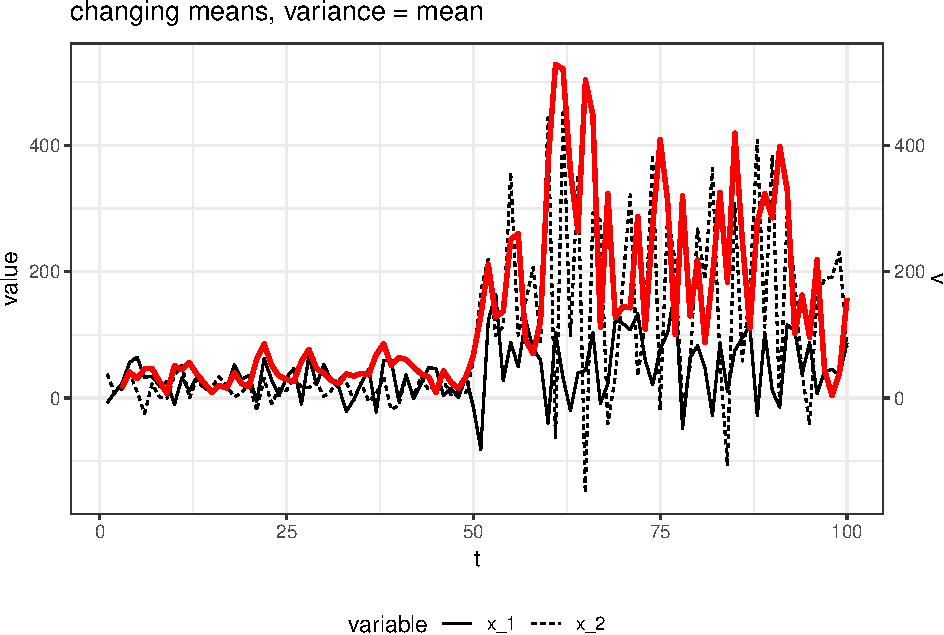
\includegraphics[width=0.65\linewidth]{06-chap-velocity_files/figure-latex/velocSysEx4-1} 

}

\caption{System change ($s$) and velocity ($v$) of the model system over the time period. Variance equal to mean ($/bar{x_i}=/sigma_i$), where means ($/bar{x}_{1_{pre}}=25$, $/bar{x}_{1_{post}}=50$, $/bar{x}_{2_{pre}}=15$, $/bar{x}_{2_{post}}=150$).}\label{fig:velocSysEx4}
\end{figure}


\end{document}
